\documentclass[a4paper,10pt]{article}
\usepackage[utf8x]{inputenc}
\usepackage[czech]{babel}

\usepackage{amsthm}
\usepackage{amsmath}
\usepackage{amsfonts}
\usepackage{mathtools}

%% číslovaný cases
\usepackage[subnum]{cases}

%% colspan a rowspan v tabulkách
\usepackage{multirow}

%%  http://tex.stackexchange.com/a/361157
\usepackage{showlabels}

%% subfigures, https://en.wikibooks.org/wiki/LaTeX/Floats,_Figures_and_Captions#Subfloats
\usepackage{subcaption}

%% číslování řádků, https://texblog.org/2012/02/08/adding-line-numbers-to-documents/
\usepackage{lineno}

%Definice, věta, důkaz!
\newtheorem{definition}{Definice}
\newtheorem{theorem}{Věta}
\newtheorem*{notation*}{Značení}
\newtheorem{note}{Poznámka}
\newtheorem{example}{Příklad}


\numberwithin{definition}{section}
\numberwithin{theorem}{section}
%\numberwithin{notation}{section}
\numberwithin{note}{section}
\numberwithin{example}{section}


%Ostatní makra
\newcommand{\TODO}[1]{ \textit{\small(zde bude doplněno: #1)} }	
\newcommand{\RLY}{?? }

\newcommand{\lattL}{\mathbb{L}}
\newcommand{\fsubsets}[1]{\mathcal{F}(#1)}

\newcommand{\term}[1]{\textit{#1}}
\newcommand{\str}[1]{{\ttfamily#1}}
\newcommand{\regex}[1]{{\ttfamily#1}}

\newcommand{\impl}[2]{{\ttfamily#1/}{\ttfamily test/data/}{\ttfamily#2}}

% Speciální nastavení

% vycentrované floating objekty
% http://tex.stackexchange.com/questions/2651/should-i-use-center-or-centering-for-figures-and-tables
\makeatletter
\g@addto@macro\@floatboxreset\centering
\makeatother

\linenumbers
\modulolinenumbers[10]


%opening
\title{Aplikace fuzzy a pravděpodobnostních automatů}
\author{Martin Jašek}
\date{12. září 2016 --- ??}

\begin{document}

\maketitle
\tableofcontents
\newpage

%%%%%%%%%%%%%%%%%%%%%%%%%%%%%%%%%%%%%%%%%%%%%%%%%%%%%%%%%%%%%%%%%%%%%%%%%%%%%%%
\section{Úvodní pojmy}
V této kapitole budou popsány základní koncepty a pojmy, bez kterých nebude možno se studiu fuzzy automatů věnovat. Bude zde tedy představen koncept fuzzy množin, pravděpodobnostního počtu a základní pojmy z teorie automatů.

%%%%%%%%%%%%%%%%%%%%%%%%%%%%%%%%%%%%%%%%%%%%%%%%%%%%%%%%%%%%%%%%%%%%%%%%%%%%%%%
\subsection{Fuzzy teorie}
Fuzzy teorie je poměrně nový pohled (oficiálně byl publikován v roce 1965\TODO{ocitovat Zadeh: Fuzzy sets}) na matematický svět. Uvažuje, že pravdivost tvrzení nenabývá jen hodnot \uv{pravda} a \uv{nepravda}, ale libovolného stupně pravdivosti (splňujícího určitá kritéria). Stejně tak, množiny (klasické neboli bivalentní) mohou prvek buďto obsahovat nebo neobsahovat. Fuzzy teorie přichází s konceptem fuzzy množin, tedy množin, které mohou prvky obsahovat jen částečně.

Svět kolem nás je jen málokdy dvojstavový, mít možnost okolí popisovat ve stupních pravdivosti je tak více, než přirozené. Například, tvrzení \uv{student učivo umí} lze těžko ohodnotit pravdou či nepravdou, pokud student z testu získal $50\%$ bodů. Naopak, říci, že \uv{student učivo umí z $1/2$} je mnohem přirozenější. 

Fuzzy teorie se toto uvažování snaží formalizovat matematicky. Na úvod si nadefinujme fuzzy množinu. 
\begin{definition}[Fuzzy množina]
 Mějme libovolnou neprázdnou množinu $U$ (tzv. univerzum). Pak zobrazení $\rho_A: U \rightarrow [0, 1]$ nazvěme členská funkce. Množinu $A$ nazýváme fuzzy množina nad $U$. Pro libovolné $x \in U$ říkáme, že prvek $x$ náleží do množiny $A$ ve stupni $\rho_A(x)$.
\end{definition}

\begin{note}
 Členská funkce nemusí být nutně zobrazení do intervalu $[0, 1]$. Interval může být nahrazen svazem s $0$ a $1$, pokud splňuje ještě některá další kritéria. Studium těchto vlastností však není účelem této práce a proto bude vynecháno. Navíc, práce s intervalem $[0 ,1]$ je poměrně výhodná z důvodu snadné implementace na počítači a proto ve všech praktických aplikacích (které jsou smyslem této práce) se bude používat právě tento interval.
\end{note}

\begin{notation*}
 Abychom rozlišili \uv{klasické} bivalentní množiny od fuzzy množin, budou fuzzy množiny v tomto textu značeny malými řeckými písmeny.
\end{notation*}

Nyní se podíváme na základní množinové operace nad fuzzy množinami.
\begin{definition}[Operace nad fuzzy množinami]
 Mějme dvě fuzzy množiny $\pi$ a $\rho$ nad univerzem $U$. Pak definujme jejich průnik, sjednocení, rovnost a inkluzi (relaci \uv{býti podmnožinou}) jako:
 \begin{align*}
  \pi \cup \rho 	\; &= \; \pi(x) \wedge \rho(x) \\
  \pi \cap \rho 	\; &= \; \pi(x) \vee \rho(x) \\
  \pi = \rho 		\; &= \; \pi(x) = \rho(x) \\
  \pi \subseteq \rho 	\; &= \; \pi(x) \le \rho(x) 
 \end{align*}
 pro všechna $x \in U$.
\end{definition}

Připomeňme, že operátory $\wedge$ $\vee$ na reálném intervalu $[0, 1]$ jsou definovány jako $\min$ a $\max$. Operátor $\le$ značí přirozené uspořádání čísel.

Množinu všech fuzzy množin nad univerzem $U$ (tedy protějšek potenční množiny u \uv{klasických} množin) budeme značit $\fsubsets{U}$. Obdobně jako u \uv{klasických} množin lze definovat kartézský součin a relace, můžeme definovat kartézký součin fuzzy množin a fuzzy relace. 

\begin{definition}[Kartézský součin fuzzy množin]
 Mějme fuzzy množiny $\rho_1, \dots, \rho_n$ nad univerzy $U_1, \dots, U_n$. Pak kartézský součin těchto fuzzy množin, psáno $\rho_1 \times \dots \times \rho_n$ nebo $\prod_{i=1}^n \rho_i$ je definován jako zobrazení $U_1 \times \dots \times U_n \rightarrow [0, 1]$.
 
\end{definition}
\begin{definition}[Fuzzy relace]
 Jako fuzzy relaci na fuzzy množinách množinách $\rho_1, \dots, \rho_n$ nazýváme libovolnou fuzzy podmnožinu kartézského součinu těchto fuzzy množin.
\end{definition}

\TODO{t-norma a konorma}.

% 
% \TODO{Zde se důkladně rozepsat o motivaci a konceptech.}
% \TODO{ZDE dát všechny ty příklady na \uv{je teplo}, \uv{je mladý} a podob. !}
% 
% Fuzzy množiny a relace budou po vzoru \cite{AstGonMenGar-FuzzAutEpsMovCmpFuzzMeasBtwStrs} nejčastěji malými řeckými písmeny (obdobně jako jejich členské (angl. \uv{membership}) funkce). Množinu všech fuzzy podmnožin množiny $S$ budeme značit $\fsubsets{S}$.

%%%%%%%%%%%%%%%%%%%%%%%%%%%%%%%%%%%%%%%%%%%%%%%%%%%%%%%%%%%%%%%%%%%%%%%%%%%%%%%
\subsection{Pravděpodobnostní počet}
(Dle potřeby rozepsat více.)\TODO{Pravděpodobnostní počet, rozepsat} \TODO{Doplnit příklady}

Z pohledu pravděpodobnostních automatů je nejzákladnějím pojmem pravděpodobnostního počtu pravděpodobnostní míra. Pravděpodobnostní míra, neboli pravděpodobnost, je reálné číslo z intervalu $[0, 1]$.  


\subsection{Fuzzy vs. pravděpodobnostní přístup} \label{subsec:FuzzyVsProb}
V předchozích dvou podkapitolých byly zavedeny základní pojmy z oblasti fuzzy teorie a pravděpodobnostního počtu. Je vidět, že jak stupeň pravdivosti, tak pravděpodobnostní míra jsou obě reálná čísla z intervalu $[0, 1]$. Oba tyto pojmy totiž popisují určitou formu neurčitosti, každá však jinou. Často však může docházet k jejich záměně.

Je však třeba mít na paměti, že tyto pojmy jsou zcela rozdílné. Stupeň pravdivosti popisuje, jak moc je tvrzení pravdivé, zatímco pravděpodobnost, jak moc je pravděpodobné, že tvrzení pravdivé bude.

Názorně je to vidět na příkladě: Trvzení \uv{Já jsem vysoký} může nabývat různých stupňů pravdivosti, avšak pravděpodobnost se nemění. Naopak tvrzení \uv{Zítra ráno mi ujede autobus} může popisovat buď zcela pravdivou skutečnost, nebo zcela nepravdivou, nicméně má smysl uvažovat, s jakou pravděpodobností tento jev nastane.

Občas se stává, že lze uplatnit oba přístupy. Například trzení \uv{Venku je pěkné počasí}. Na jednu stranu se můžeme bavit o \uv{pěknosti} počasí (tj. jak moc je venku pěkně). Ovšem na druhou stranu můžeme uvažovat, že autor výroku není seznámen s aktuálním počasím a proto může určovat s jakou pravděpodobností venku skutečně je pěkně. Právě z takovýchto situací pramení časté záměny těchto dvou přístupů.

%%%%%%%%%%%%%%%%%%%%%%%%%%%%%%%%%%%%%%%%%%%%%%%%%%%%%%%%%%%%%%%%%%%%%%%%%%%%%%%
\subsection{Popis v přirozeném jazyce}
Vzhledem k tomu, že účelem této práce je studovat uplatění fuzzy a pravděpodobnostních automatů v praxi, je nutné zavést nástroj pro přemostění \uv{propasti} mezi fuzzy teorií (pravděpodobnostním počtem) a popisem v přirozeném jazyce.

Pravděpodobnostní počet k tomuto účelu používá jevy. Je poměrně přirozené říkat \uv{Pravděpodobnost jevu $e$ je $p$.}.

Pro popis stupňů pravdivosti by bylo možné používat \uv{Tvrzení $t$ je pravdivé ve stupni $d$.}. Bude však výhodnější použít tzv. lingvistické proměnné \cite{Zad-ConLingVarAppApprRea}. Každá lingvistická proměnná $\alpha$ je tvořena univerzem $U$ hodnot a množinou lingvistických štítků $T$. Pro každý štítek $X \in T$ pak definuje jeho význam $M(X)$, fuzzy množinu nad $U$ (tj. funkci, která hodnotě z univerza přiřadí stupeň pravdivosti). Fakt, že lingvistická proměnná $\alpha$ nabývá \uv{hodnoty} $X$ budeme zapisovat $\alpha = X$.

\begin{example}
 Mějme lingvistickou proměnnou $\alpha$ s významem \uv{výška osoby}. Univerzem hodnot jsou všechna nezáporná reálná čísla. Lingvistické štítky jsou \uv{malá}, \uv{střední}, \uv{vysoká} a \uv{velmi velká}. Význam jednotlivých štítků je vyobrazen na obrázku \ref{fig:lingVarsMeansChart}.

 Osoba $X$ má výšku $h$. Namísto \uv{Platnost tvrzení \uv{osoba $X$ má střední výšku} je ve stupni $M(\text{střední})(h)$} můžeme říkat \uv{osoba $X$ má střední výšku}. Symbolicky zapsáno: $\alpha = \text{střední}$.
\end{example}

\begin{figure}
 \centering
 \includegraphics{charts0}
 
 \caption{Graf významových funkcí štítků \uv{malá}, \uv{střední}, \uv{velká} a \uv{velmi velká}} \label{fig:lingVarsMeansChart}
\end{figure}

Pro popis složitějších zákonitostí je potřeba pokročilejčí nástroj. Vztahy tak budeme popisovat pomocí tzv. fuzzy \ifthen pravidel. Klasické bivalentní \ifthen pravidlo je výrok: je tvaru:
$$
 \text{Jestliže $x_1$, $\dots$, $x_n$, pak $y$}
$$
kde $x_1, \dots x_n, y$ jsou podvýroky\footnote{Zapíšeme-li \ifthen pravidlo jako formuli, obdržíme Hornovskou klauzuli. Můžeme tak určit pravdivost jejího důsledku $y$ na základě pravdivosti předpokladů $x_1, \dots, x_n$.}.

\begin{example}
 Následující výroky jsou \ifthen pravidla:
 \begin{itemize}
  \item Jestliže je spínač sepnut, pak žárovka svítí
  \item Jestliže je $\text{věk}(p) < 15$, pak $p$ je dítě
  \item Je-li $x \in \mathbb{N}$, $x > 2$, $\nexists y < x: y|x$, pak $x$ je prvočíslo
 \end{itemize}
\end{example}

Fuzzy \ifthen pravidla pak budou vypadat následovně:
$$
 \text{Jestliže $\alpha_1 = x_1$, $\dots$, $\alpha_n = x_n$, pak $\beta = y$}
$$
kde $\alpha_1, \dots \alpha_n, \beta$ jsou lingvistické proměnné a $x_1, \dots, x_n, y$ jsou jejich štítky.


\begin{example}
 Uvažujme systém, u kterého známe tlak (lingvistická proměnná $\alpha_t$) a teplotu (lingvistická proměnná $\alpha_p$) a popisujeme úroveň otevření ventilu (lingvistická proměnná $\alpha_v$). 
 Označme štítky $p_L$ (\uv{tlak je nízký}), $p_N$ (\uv{tlak je normální}), $p_H$ (\uv{tlak je vysoký}) a dále $t_N$ (\uv{teplota je v normě}) a $t_H$ (\uv{teplota je zvýšená}). Konečně zaveďme štítky $v_O$ (\uv{ventil je uzavřen}) a $v_C$ (\uv{ventil je otevřen}). 
 
 Pak pravidla
 \begin{align*}
  \text{Pokud je tlak nízký a teplota zvýšená, }&\text{pak ventil je uzavřen} \\
  \text{Pokud je tlak vysoký a teplota v normě, }&\text{pak ventil je otevřen}
 \end{align*}

 mohou být přepsána jako
 \begin{align*}
  \text{Jestliže } \alpha_p = p_L, \alpha_t = t_H &\text{ pak } \alpha_v = v_C \\
  \text{Jestliže } \alpha_p = p_H, \alpha_t = t_N &\text{ pak } \alpha_v = v_O 
 \end{align*}
\end{example}


%%%%%%%%%%%%%%%%%%%%%%%%%%%%%%%%%%%%%%%%%%%%%%%%%%%%%%%%%%%%%%%%%%%%%%%%%%%%%%%
\subsection{Základní pojmy z teorie automatů}
Definice a značení následujících pojmů jsou převzaty z \cite{Koz-AutComp}.

% \subsubsection*{Abeceda}
Základním pojmem při studiu automatů je abeceda. Abeceda je neprázdná a konečná množina symbolů a značí se typicky $\Sigma$, případně jiným velkým písmenem řecké abecedy. Abecedou může být například \uv{všechna malá písmena latinky}, nebo např. číslice $0$ -- $9$.

% \subsubsection*{Řetezec}
Posloupnost $u = a_1 a_2 \dots a_n$ kde $a_1,  a_2, \dots, a_n \in \Sigma$ se nazývá řetězec $u$ nad abecedou $\Sigma$. Číslo $n$ je pak délka řetězce $u$, která se jinak značí $|u|$. Řetězec, který má nulovou délku, značíme $\varepsilon$.

Řetězec $u \circ v = a_1 \dots a_n b_1 \dots b_m$ (častěji však $uv$) se nazývá zřetězení (konkatenace) řetězců $u = a_1 \dots a_n$ a $v = b_1 \dots b_m$. Přirozeně platí $|uv| = n + m$. Jako $n$-tá mocnina $u^n$ řetězce $u$ se označuje řetezec:
$$
  u^n = \begin{dcases}
    \varepsilon & \text{pokud } n = 0\\
    u u^{n-1} & \text{jinak}
  \end{dcases}
$$

Symbolem $\Sigma^*$ se značí množina všech řetězců nad abecedou $\Sigma$ (včetně $\varepsilon$). Symbol $\Sigma^+$ pak značí všechny řetězce nad abecedou $\Sigma$ vyjma $\varepsilon$. %Symbol $\Sigma^*$ se nazývá Kleeneho uzávěř, $\Sigma^+$ pak pozitivní uzávěř.

%%%%%%%%%%%%%%%%%%%%%%%%%%%%%%%%%%%%%%%%%%%%%%%%%%%%%%%%%%%%%%%%%%%%%%%%%%%%%%%
% \subsection{Jazyky}

Pojmem (formální) jazyk se označuje určitá vybraná množina $L$ řetězců nad abecedou $\Sigma$, tj. $L \subseteq \Sigma^*$.

Nad jazyky $L$, $L_1$ a $L_2$ nad abecedami $\Sigma$, $\Sigma_1$ a $\Sigma_2$ se zavádí:
$$
\begin{array}{ll}
  L_1 L_2 		= \left\{ u v \,|\, u \in L_1, v \in L_2 \right\}	& \text{zřetězení (produkt)}	\\ \\
  L^n 			= \begin{dcases}
      \left\{ \varepsilon \right\} 	& \text{pokud } n = 0 \\
      L L^{n-1} 			& \text{jinak}
    \end{dcases} 								& \text{$n$-tá mocnina}		\\ \\
  
  L^* 	= \bigcup\limits_{i=0}^{\infty} L^i						& \text{Kleeneho uzávěr}	\\ \\
  L^+ 	= \bigcup\limits_{i=1}^{\infty} L^i						& \text{pozitivní uzávěr}
\end{array}
$$

Je-li jazyk konečná množina, tj, obsahuje konečně mnoho řetězců, nazýváme jej konečný. V opačném případě říkáme, že je jazyk nekonečný.

Podobně, jako jsme si zavedli fuzzy množinu jako protějšek \uv{klasické} množiny, můžeme nadefinovat i fuzzy jazyk. Fuzzy jazyk nad abecedou $\Sigma$ je její libovolná fuzzy podmnožina, tj. $\lambda \in \fsubsets{\Sigma^*}$. \TODO{a co probabilistický jazyk?}



\section{Definice fuzzy automatu}
V této kapitole bude podrobně popsán a formálně nadefinován \uv{fuzzy automat} a proces jeho výpočtu. Pro snažší ilustraci bude nejdříve popsán automat bivalentní a následně upraven do podoby fuzzy automatu. Popis bivalentního automatu je převzat z \cite{HopUl-IntrAutTheLangComp}, popis fuzzy automatu z \cite{GonGar-FuzzLangInfRanAccGuzzAutPumLemDetProc} (pokud není uvedeno jinak).

Hned na úvod je třeba zdůraznit terminologii. Jak bývá u automatů zvykem, pojem \uv{automat} označuje souhrnně různé varianty automatů, typicky nedeterministický i deterministický, bez dalšího rozlišování. Vzhledem k tomu, že základním (a nejpoužívanějším) fuzzy automatem je automat nedeterministický, bude proto druhá polovina této kapitoly věnována právě nedeterministickému fuzzy automatu. Zbývající známé varianty fuzzy automatů budou poté shrnuty v následujcí kapitole.

\TODO{někde tady zdůraznit konečné (ve smyslu konečnosti automatu) automaty?}

%%%%%%%%%%%%%%%%%%%%%%%%%%%%%%%%%%%%%%%%%%%%%%%%%%%%%%%%%%%%%%%%%%%%%%%%%%%%%%%
\subsection{Koncept automatu}
Automat se řadí mezi tzv. výpočetní modely. Výpočetní model je označení pro matematický formalizmus, který popisuje určitý výpočet, algoritmus. Spolu s automaty (ve všech jejich variantách a modifikacích) se k výpočetním modelům řadí například také Turingovy stroje \cite{MorMal-FuzzyAutLang}. 

Automaty také často bývají nazývany jako stavové stroje. Na automat lze totiž nahlížet jako na určité zařízení. Toto zařízení je charakterizováno svým vnitřním stavem a v závislosti na vstupu se tento stav diskrétně mění, tj. můžeme tvrdit, že automat přecháhází od jednoho stavu k jinému.

Důležité je také dělení automatů na deterministické a nedeterministické. Obecná definice říká, že u deterministického automatu je jednoznačně dáno, do kterého stavu v každý moment výpočtu automat přejde. Naopak u nedeterminstického tento předpoklad neplatí, tj. výpočet automatu se může octnout v situaci, kdy má možnost přejít do dvou a více stavů \uv{současně}.

Tuto situaci budeme u nedeterministických automatů reprezentovat tak, že automat se nebude nacházet vždy v jednom stavu, ale jeho aktuální stav bude popsán celou množinou stavů, ve kterých se nachází.

Automat tedy musí zcela určitě obsahovat stavy, ve kterých se při svém výpočtu může nacházet. Spolu s nimi je každý automat dán vstupy, se kterými dokáže pracovat. Vstupy pro automat budou řetězce nad nějakou danou abecedou. O popis přechodů mezi stavy se bude starat přechodová funkce.

Dále, u každého automatu musí být stanoven počáteční stav. Vzhledem k tomu, že se budeme bavit o automatu nedeterministickém, budeme uvažovat množinu počátečních stavů.

Automaty původně vznikly jako nástroje pro rozpoznávání určité třídy jazyků\footnote{Konkrétně, jedná se o tzv. regulérní jazyky, které budou popsány v kapitole \TODO{doplnit odkaz}}. To znamená, že automat musí pro libovoný řetězec, zda-li do uvedeného jazyka patří nebo ne. U automatů je toto řešeno pomocí tzv. koncových stavů. Pokud výpočet automatu zkončí v koncovém stavu, pak je řetězec automatem zpracovávaný přijat, v opačném případě zamítnut.

Nyní máme známu obecnou představu, jak by měl automat vypadat. Následuje tedy definice nedeterministického bivalentního automatu, spolu se stručným popisem jeho činnosti. Následně je pak odvozena definice nedeterministického fuzzy automatu a jeho výpočtu.

\TODO{potenční množina -- bivalentní značím $2^M$, fuzzy $\fsubsets{M}$, nechtělo by to sjednotit a používat taky $P(M)$, resp. $\mathcal{P}(M)$?}

%%%%%%%%%%%%%%%%%%%%%%%%%%%%%%%%%%%%%%%%%%%%%%%%%%%%%%%%%%%%%%%%%%%%%%%%%%%%%%%
\subsection{Nedeterminstický bivalentní automat}
Nedeterministický bivalentní automat je definován následovně:

\begin{definition}[Nedeterministický bivalentní automat]\label{def-NedBivAut}
 Nedeterministický bivalentní automat $A$ je pětice $(Q, \Sigma, \mu, I, F)$, kde $Q$ je konečná množina stavů, $\Sigma$ je abeceda, $\mu: Q \times \Sigma \rightarrow 2^Q$ je přechodová funkce a $I \subseteq Q$ a $F \subseteq Q$ je množina počátačních a koncových stavů.
\end{definition}

\TODO{reprezentace? příklad?}

Výpočet automatu, tedy zpracování vstupního řetězce, je definován jako posloupnost konfigurací. Konfigurace je přesný popis aktuálního stavu výpočtu (tzn. nezpracovaná část vstupního řetězce a množina stavů, ve kterých se automat nachází). Na počátku se výpočet nachází v tzv. počáteční konfiguraci, tj. nezpracovanou částí celého řetězce je celý vstupní řetězec a množinou stavů, ve kterých se automat nachází je celá množina $I$.

Automat čte ze vstupu postupně symboly. Pokud se automat nachází ve stavu $q$ a právě přečteným symbolem je symbol $a$, pak automat přechází do stavu $q'$ (a symbol $a$ je ze vstupu odebrán) pokud $q' \in \mu(q, a)$. Vyprázdní-li takto automat celý vstup (na vstupu je prázdný řetězec), ocitá se v tzv. koncové konfiguraci. Pokud alespoň jeden ze stavů, ve kterém se automat nachází, je koncový, nazývá se tato konfigurace přijímací, v opačném případě zamítací.

Pokud výpočet automatu pro řetězec $w$ zkončí přijímací konfigurací, říkáme, že automat řetězec přijímá. Pokud zkončí zamítací konfigurací, pak říkáme, že je řetězec zamítán. Jazyk rozpoznávaný automatem je pak množina takových řetězců $w \in \Sigma^*$, které automat přijímá.

Ekvivalentním způsobem, jak určit, zda-li je řetězec automatem přijímán či zamítán je pomocí rozšířené přechodové funkce $\mu^*: 2^Q \times \Sigma^* \rightarrow 2^Q$. Rozšířenou přechodovou funkci $\mu^*$ tak lze číst \uv{nachází-li se automat v množině stavů $Q'$ a na vstupu je řetězec $w$, pak automat přejde do množiny stavů $\mu^*(Q'', w)$}. \TODO{uvést její předpis?} 

Následuje popis, jak pojmy týkající se nedeterministického bivalentního automatu \uv{zobecnit} na odpovídající pojmy z oblasti fuzzy automatů. 

%%%%%%%%%%%%%%%%%%%%%%%%%%%%%%%%%%%%%%%%%%%%%%%%%%%%%%%%%%%%%%%%%%%%%%%%%%%%%%%
\subsection{Nedeterministický fuzzy automat}
Stejně tak, jak fuzzy množiny jsou zobecněním klasických \uv{bivalentních} množin, dá se předpokládat, že i fuzzy automaty budou v určitém smyslu zobecněním klasických bivalentních automatů. A nebude tomu jinak ani u nedeterministického automatu.

Vzhledem k tomu, že automat je definován jako struktura, je zprvu třeba stanovit, které její části má smysl zobecňovat na fuzzy množiny (relace, funkce). Abeceda symbolů i množina stavů zcela určitě můsí zůstat zachovány jako konečné bivalentní množiny. U přechodové funkce naopak očekáváme ostupňovanost (očekáváme možnost říkat \uv{automat přejde do stavu $q$ ve stupni $d$}). Co se počátečních a koncových stavů týče, někde se lze setkat s reprezentací bivalentní množinou (např. v. \cite{AndAbdAsm-ApprPattMatcFuzzLog}, \cite{SnaKepAbrHas-AproxStriMatchFuzzAut}), jinde zase s fuzzy množinami (\cite{StaCir-ConsFuzzAutFuzzRegExp}, \cite{AstGariGonVillFar-ApprStrMatUsiDefFuzzAutLearExpr}, \cite{Bel-DetAndFuzzAut} \cite{GonGar-FuzzLangInfRanAccGuzzAutPumLemDetProc})\footnote{Jak bude ukázáno, mezi oběma druhy automatů existuje ekvivalence. Automaty s bivalentními počátečními a koncovými stavy se však jednoduššeji reprezentují.}. Vzhledem k tomu, že druhý jmenovaný, tj. automat s fuzzy množinou vstupních i 
výstupních stavů, je zřejmě obecnější, bude nadále uvažován pouze tento.

\begin{definition}[Nedeterministický fuzzy automat]\label{def-ZaklDefNedFuzzAut}
 Nedeterministický fuzzy automat $A$ je pětice $(Q, \Sigma, \mu, \sigma, \eta)$, kde $Q$ je konečná množina stavů, $\Sigma$ je abeceda, $\mu$ je fuzzy přechodová funkce (fuzzy relace $Q \times \Sigma \times Q \rightarrow [0, 1]$) a $\sigma$ a $\eta$ jsou po řadě fuzzy množiny nad $Q$ počátačních, resp. koncových stavů.
\end{definition}

\subsection{Reprezentace nedeterministického fuzzy automatu}
Nedeterministické fuzzy automaty se typicky reprezentují třemi způsoby. Prvním z nich je přechodová tabulka (např. \cite{DooKre-NewDirFuzzAut}). 

Jedná se o tabulku, která v řádcích obsahuje aktuální stavy a ve sloupcích následující stavy (tím je dána množina stavů). Poté buňka na řádku $q$ a ve sloupci $q'$ obsahuje $\mu(q, q') \in \Sigma \rightarrow [0, 1]$, tj. výčet symbolů a stupňů pravdivosti těchto přechodů. Dále tabulka obsahuje dva dodatečné sloupce pro určení stupně počátečního a koncového stavu každého stavu.

Tabulka však často může být rozsáhlá, proto se reprezentace tabulkou často nahrazuje maticovým způsobem (např. \cite{SnaKepAbrHas-AproxStriMatchFuzzAut}, \cite{StaCir-ConsFuzzAutFuzzRegExp}). Uvažujme označení stavů $Q = \{ q_0, \dots q_n \}$. Dále, přechodovou funkci $\mu$ rozložme na soubor funkcí $\mu_x$ pro všechny $x \in \Sigma$ takové, že $\mu_x(q, q') = \mu(q, x, q')$. Pro každý symbol $x \in \Sigma$ vytvoříme matici tak, že na $i$-tém řádku a $j$-tém sloupci obsahuje hodnotu $\mu(q_i, x, q_j)$. Dále je přiložen vektor počátečních (koncových) stavů takový, že $i$-tá složka vektoru je rovna hodnotě $\sigma(q_i)$ ($eta(q_i$).

Posledním používaným způsobem je grafická reprezentace (např. \cite{DooKre-NewDirFuzzAut}, \cite{GonGar-FuzzLangInfRanAccGuzzAutPumLemDetProc}, \cite{StaCir-ConsFuzzAutFuzzRegExp}). Jedná se o orientovaný ohodnocený graf, kde:
\begin{itemize}
 \item stavy automatu tvoří uzly grafu
 \item každý uzel stavu $q$ je označen $q/\eta(q)$
 \item hrana od uzlu $q$ k uzlu $q'$ je ohodnocena seznamem takových $x/d$, pro které platí $\mu(q, x, q') = d$
 \item každý uzel $q$ je označen šipkou vedoucí k tomuto uzlu ohodnocenou hodnotou $\sigma(q)$
\end{itemize}

Pokud je některý ze stupňů roven $0$, tak se v grafu zpravidla vynechává.

\begin{example}
 \TODO{vymyslet příklad}
\end{example}

\subsection{Výpočet nedeterministického fuzzy automatu}
Výpočet nedeterminsitického fuzzy automatu vychází z výpočtu nedeterministického bivalentního automatu. U bivalentního automatu jsme uvažovali, že automat se může nacházet ve více stavech současně, tj. součástí konfigurace výpočtu je množina stavů, ve kterých se automat nachází. Nedeterministický fuzzy automat se této koncepce drží, jen ji obohacuje o odstupňovanost. Tedy, že množina stavů, ve kterých se automat může nacházet je fuzzy množinou. Tutu množinu budeme nazývat fuzzy stav.

\begin{definition}[Fuzzy stav]\label{def-FuzzStav}
 Mějme nedeterministický fuzzy automat $A$. Pak jako fuzzy stav označujeme každou fuzzy podmnožinu jeho stavů, tj. $\widehat{Q} \in \fsubsets{Q}$.
\end{definition}

\begin{note}
 Fuzzy množiny počátečních a koncových stavů jsou ve své podstatě také fuzzy stavy.
\end{note}

Obdobně jako u bivalentního automatu, nezpracovaná část řetězce na vstupu spolu s (fuzzy) množinou stavů, ve kterých se automat nachází, označujeme jako konfigurace automatu. Posloupnost konfigurací nazýváme výpočtem. Formální definice výpočtu je však mírně složitější a pro jeho zavedení bude potřeba pár dalších pojmů, které budou nyní uvedeny.

\begin{definition}[Konfigurace nedeterministického fuzzy automatu]
  Mějme nedeterminsitický fuzzy automat $A$. Pak každý prvek $(w, \widehat{Q})$ relace $\Sigma^* \times \fsubsets{Q}$ nazýváme konfigurace automatu $A$.
\end{definition}


\begin{definition}[Aplikace fuzzy relace na fuzzy stav (tzv. t-kompozice)]
 Mějme nedeterministický fuzzy automat $A$ a fuzzy stav $\widehat{Q}$. Pak aplikací binární fuzzy relace $R: Q \times Q \rightarrow [0, 1]$ na fuzzy stav $\widehat{Q}$ obdržíme fuzzy symbol $\widehat{Q} \circ R$ splňující pro každé $p \in Q$: $(\widehat{Q} \circ R )(p) = \max_{q \in Q} (\widehat{Q}(q) \otimes R(q, p))$.
 
  \TODO{přesunout do některé z úvodních kapitol?}
  \TODO{t-kompozice má pár dalších zajímavých (a potřebných) vlastností (např. asociativitu)}
\end{definition}

\begin{notation} \ref{not:muOverSym}
 Označme $\mu[x](p, q) = \mu(p, x, q)$.
\end{notation}

\begin{definition}[Přechodová funkce fuzzy stavů]\label{def-PreFunFuzzStav}
 Mějme nedeterministický fuzzy automat $A$. Pak přechodová funkce fuzzy stavů je fuzzy relace $\widehat{\mu}: \fsubsets{F} \times \Sigma \rightarrow \fsubsets{F}$ taková, že pro každý fuzzy stav $\widehat{Q} \in \fsubsets{Q}$ a symbol $x \in \Sigma$ je $\widehat{\mu}(\widehat{Q}, x) = \widehat{Q} \circ \mu[x]$.
\end{definition}

\begin{definition}[Výpočet nedeterministického fuzzy automatu]
  Mějme nedeterminsitický fuzzy automat $A$. Každou posloupnost konfigurací $(w_0, \widehat{Q}_0), \dots, (w_m, \widehat{Q}_m)$ splňující pro každé $0 \leq i < m$
  \begin{enumerate}
   \item $w_{i} = a w_{i+1}$ kde $a \in \Sigma$
   \item $\widehat{Q}_{i+1} = \widehat{Q}_{i} \circ \widehat{\mu}(\widehat{Q}_{i}, a)$
  \end{enumerate}
  nazýváme výpočet automatu $A$ z fuzzy stavu $\widehat{Q}_0$ při vstupu $w_0$.
\end{definition}

Vidíme, že výpočet je definován rekurentně. Zápis můžeme přetransformovat do podoby rozšířené přechodové funkce \cite{IgnCirBog-DetFuzAutMemValComResLat}.

\begin{definition}[Rozšířená přechodová funkce]\label{def-RozPreFunFuzzStav}
 Mějme nedeterministický fuzzy automat $A$. Pak rozšířená přechodová funkce je fuzzy relace $\mu^*: Q \times \Sigma^* \times Q \rightarrow [0,1]$ daná následujícím předpisem:
 
 \begin{enumerate}
  \item $\mu^*(q, \epsilon, q) = 1$ pro všechna $q \in Q$
  \item $\mu^*(q, u a, q') =  \bigvee_{p \in Q} \mu^*(q, u, p) \otimes \mu(p, a, q')$ pro všechna $q, q' \in Q, u \in \Sigma^*, a \in \Sigma$
  %\item $\mu^*(q, w, q') =  0$ pro všechny ostatní $q, q' \in Q$ a $w \in \Sigma^*$
 \end{enumerate}
\end{definition}

Rozšířená přechodová funkce fuzzy stavů zřejmě plní funkci výpočtu automatu. Výraz $\mu^*(q, w, q')$ odpovídá stupni, v jakém automat přejde při zpracování řetězce $w$ ze stavu $q$ do stavu $q'$. 

Stupeň $A(w)$, v jakém je řetězec $w$ automatem $A$ přijat je dán jako nejvyšší stupeň pro všechny dvojice stavů $p, q$:
\begin{enumerate}
 \item stupňem \uv{stav $q$ je počáteční ve stupni $\sigma(q)$}
 \item stupňem \uv{automat při vstupu $w$ přejde ze stavu $q$ do stavu $q'$ ve stupni $\mu^*(q, w, q')$}
 \item stupňem \uv{stav $q'$ je koncový ve stupni $\eta(q')$}
\end{enumerate}

Můžeme tedy zapsat:

\begin{definition}[Řetězec přijímaný automatem]\label{def-RetPriAut}
 Mějme nedeterministický fuzzy automat $A$. Pak řětězec $w \in \Sigma^*$ je automatem $A$ přijat ve stupni
 \begin{align} \label{eq-RetPriAut}
  A(w) = \max_{q, q' \in Q} (\sigma(q) \otimes \mu^*(q, w, q')(q) \otimes \eta(q'))
 \end{align}
\end{definition}


\begin{note}
  V literatuře (např. \cite{SebJoh-InvFuzzAutInvFuzzLang} \cite{IgnCirBog-DetFuzAutMemValComResLat} \cite{Bel-DetFuzAut}) se obvykle lze setkat s \uv{techničtějším} zápisem ať už jen rozšířené přechodové funkce, tak $A(w)$. Pro řetězec $w = a_0 \dots a_n$ rozvojem rekurence $\mu^*$ a použitím asociativity $\circ$ můžeme napsat:
  \begin{align*}
   \mu^*(q, a_0 \dots a_n, q') 
    &= \bigvee_{p_n \in Q} \left( \dots \bigvee_{p_0 \in Q} (1 \otimes \mu(p_0, a_0, p_1)) \dots \otimes \mu(p_n, a_n, q') \right)  \\
    &= \bigvee_{p_n \in Q} \dots \bigvee_{p_0 \in Q} \mu(p_0, a_0, p_1) \dots \otimes \mu(p_n, a_n, q') \\
    &= \bigvee_{(p_n,\dots, p_0) \in Q^n} \mu(p_0, a_0, p_1) \dots \otimes \mu(p_n, a_n, q')
  \end{align*}
  Poté může být (\ref{eq-RetPriAut}) zapsána jako:
  $$
    A(a_0 \dots a_n) = \bigvee_{(p_n,\dots, p_0, q') \in Q^{n+1}} (\sigma(p_0) \otimes \mu(p_0, a_0, p_1) \dots \otimes \mu(p_n, a_n, q') \otimes \eta(q'))
  $$
  
  Tento zápis intuitivněji popsuje výpočet automatu. Tento zápis totiž můžeme číst jako: \uv{Řetězec je přijímán ve stupni $A(a_0 \dots a_n)$ jestliže ze stavu $p_0$, který je počáteční ve stupni $\sigma(p_0)$ přejde přečtením $a_0$ do $p_1$ ve stupni $\mu(p_0, a_0, p_1)$, $\dots$, ze stavu $p_n$ přečtením $a_n$ do stavu $q'$ ve stupni $\mu(p_n, a_n, q')$, a stav $q'$ je koncový ve stavu $\eta(q')$.}
  
  Z tohoto zápisu je také patrné, že výpočet $A(a_0 \dots a_n)$ dle definice vyžaduje $|Q|^{n+1}$ výpočtů, každý o délce $1 + n + 1$ elementárních kroků. Výpočet má tedy exponenciální složitost vzhledem k délce vstupního řetězce.
  
\end{note}

Podobně, jak u bivalentních automatů, jazyk rozpoznávaný automatem je množina všech řetězců, které jsou tímto automatem rozpoznávané. U fuzzy automatu se však bude pochopitelně jednat o fuzzy jazyk.

\begin{definition}[Jazyk rozpoznávaný automatem]\label{def-JazRozpAut}
 Mějme nedeterministický fuzzy automat $A$. Pak fuzzy množinu $L(A)(w) = A(w)$ nad univerzem $\Sigma^*$ nazýváme fuzzy jazyk rozpoznávaný automatem $A$.
\end{definition}

\TODO{Jazyk rozpoznávaný automatem značit $\mathcal{L}$ nebo jen $L$? A automat $\mathcal{A}$, $\mathbf{A}$, $\mathbb{A}$ nebo jen $A$?}


%%%%%%%%%%%%%%%%%%%%%%%%%%%%%%%%%%%%%%%%%%%%%%%%%%%%%%%%%%%%%%%%%%%%%%%%%%%%%%%
%%%%%%%%%%%%%%%%%%%%%%%%%%%%%%%%%%%%%%%%%%%%%%%%%%%%%%%%%%%%%%%%%%%%%%%%%%%%%%%
%%%%%%%%%%%%%%%%%%%%%%%%%%%%%%%%%%%%%%%%%%%%%%%%%%%%%%%%%%%%%%%%%%%%%%%%%%%%%%%
\section{Varianty fuzzy automatů}
V této kapitole budou uvedeny další typy fuzzy automatu. Kromě nedeterminstického fuzzy automatu, kterému byla věnována předchozí kapitola, se v souvislosti s fuzzy automaty často mluví s o dalších výpočetních modelech. A právě ty jsou předmětem této kapitoly. 

Vzhledem k tomu, že se obvykle jedná o modifikace elementární, nebudou rozebírány do hloubky. Podrobnější informace o těchto automatech jsou k nalezení v literatuře.

%%%%%%%%%%%%%%%%%%%%%%%%%%%%%%%%%%%%%%%%%%%%%%%%%%%%%%%%%%%%%%%%%%%%%%%%%%%%%%%
\subsection{Deterministický fuzzy automat}
V teorii \uv{klasických} bivaletních automatů se rozlišuje automat deterministický a nedeterministický. Deterministcký automat je charakterizován tím, že každý krok jeho výpočtu je jednoznačně určen. U nedeterministického tento předpoklad platit nemusí. Právě z tohoto důvodu je deterministický automat klíčovým pojmem v oblasti \uv{klasických} bivaletních automatů, zatímco nedeterministický jeho zobecnění.

U fuzzy automatů tomu je přesně naopak. Deterministický fuzzy automat se obvykle definuje pouze jako speciální případ nedeterministického. Podobně jako u nedeterministického automatu existuje několik různých definic. V \cite{Bel-DetFuzAut} je definován jako deterministický bivalentní automat, jen koncové stavy jsou fuzzy. Dle \cite{LiLiLi-RelAmoSevTypFuzAut} je to deterministický bivalentní automat, ale s fuzzy počátečními stavy, koncovými stavy i přechodovu funkcí.

V \cite{GonGar-FuzzLangInfRanAccGuzzAutPumLemDetProc} definují determinsitický fuzzy automat jako nedeterministický fuzzy automat s tím, že je doplněn o omezení přechodové funkce, že z každého stavu při každém vstupním symbolu automat může přejít do nejvýše jednoho stavu.

Deterministické fuzzy automaty mají význam především pro implementace. Jak bylo zmíněno v předchozí kapitole, \TODO{zmínit složitost (popř. ověřit, že byla zmíněna)} časová složitost výpočtu nedeterminstického fuzzy automatu je exponenciální vzhledem k délce vstupu. U deterministického automatu je tato složitost lineární. Bohužel, zpravidla bývá vykoupena mnohonásobně vyšším počtem stavů automatu.

U všech tří citovaných definic deterministického fuzzy automatu jsou uvedeny algoritmy pro tzv. determinizaci automatu, tedy převod nedeterministického fuzzy automatu na jemu odpovídající deterministický. Algoritmus podle \cite{GonGar-FuzzLangInfRanAccGuzzAutPumLemDetProc} byl naimplementován\TODO{opsat ho?}.

%%%%%%%%%%%%%%%%%%%%%%%%%%%%%%%%%%%%%%%%%%%%%%%%%%%%%%%%%%%%%%%%%%%%%%%%%%%%%%%
\subsection{Nedeterminstický fuzzy automat s $\epsilon$-přechody}
Nedeterminstický fuzzy automat s $\epsilon$-přechody je rozšíření nedeterminsitického fuzzy automatu. Toto rozšíření je realizováno pomocí tzv. $\epsilon$-přechodů. \uv{Klasický} přechod automat při svém výpočtu realizuje, je-li na vstupu symbol odpovídající symbolu pravidla. Oproti tomu $\epsilon$-přechod však automat může realizovat kdykoliv, bez ohledu na symbol na vstupu.

Takovýto automat nalézá uplatnění především v praktických aplikacích. S jeho pomocí lze velmi elegantně vyřešit např. rozdvojejí výpočtu nebo přesun výpočtu do jiného stavu, a to bez ohledu na vstup. Formální definice tohoto automatu lze nalést např. v \cite{SnaKepAbrHas-AproxStriMatchFuzzAut} či \cite{LiLiLi-RelAmoSevTypFuzAut}.

%%%%%%%%%%%%%%%%%%%%%%%%%%%%%%%%%%%%%%%%%%%%%%%%%%%%%%%%%%%%%%%%%%%%%%%%%%%%%%%
\subsection{Zobecněný automat}
V kapitole \ref{subsec:FuzzyVsProb} byl rozebírán koncepční rozdíl mezi stupněm pravdivosti a pravděpobností. V teorii fuzzy/pravděpodobnostních automatů existují snahy tyto dva přístupy sloučit. Vniklo proto několik definic tzv. zobecněného automatu, např. \cite{DooKre-NewDirFuzzAut} či Max-Min automat \cite{San-MaxAut}. 

Hodnota reprezentující neučitost (tj. stupeň pravdivosti nebo pravděpodobnost) se u těchto automatů nazývá širším pojmem \uv{váha}. Tomuto druhu automatů se proto někdy říká automat s váhami.

%%%%%%%%%%%%%%%%%%%%%%%%%%%%%%%%%%%%%%%%%%%%%%%%%%%%%%%%%%%%%%%%%%%%%%%%%%%%%%%
\subsection{Fuzzy automat s výstupem}
Rožšířením klasického automatu lze získat automat s výstupem. Automat kromě přechodové funkce disponuje také výstupní přechodovou funkcí, která při přechodu mezi stavy odesílá na výstup symboly. Automat s výstupem tak obvykle nemá koncové stavy. S fuzzy automaty s výstupem se lze setkat např. v \cite{BlaDelPeg-FuzzAutIndUsNeuNet}\cite{PedGac-LeaFuzzAut}\cite{BlaDelPeg-FuzzGraIntUsiNeuNet}\cite{CheMo-MinAlgFuzFinAut}\cite{ThoMar-DetAccRegFuzLang}.

%%%%%%%%%%%%%%%%%%%%%%%%%%%%%%%%%%%%%%%%%%%%%%%%%%%%%%%%%%%%%%%%%%%%%%%%%%%%%%%
\subsection{Stavový stroj}
V určitém smyslu opakem fuzzy automatu s výstupem je stavový stroj. Oproti němu totiž výstupní schopnosti běžného fuzzy automatu nerozšiřuje, ale naopak ubírá. Stavový stroj je totiž výpočetní model, který nedisponuje žádnou formou výstupu\footnote{V určitém smyslu však může být za výstup považován stav (resp. fuzzy stav). ve kterém výpočet zkončil.}. U stavových strojů není totiž důležitý výsledek výpočtu, ale jeho průběh.

Takovýto automat je uveden např. v \cite{Qiu-ChaFuzFinAut}.

%%%%%%%%%%%%%%%%%%%%%%%%%%%%%%%%%%%%%%%%%%%%%%%%%%%%%%%%%%%%%%%%%%%%%%%%%%%%%%%
\subsection{Událostmi řízený fuzzy automat} \label{subsec:FuzzEvMach}
Jako událostmi řízený fuzzy automat se obvykle označuje další třída výpočetních modelů, které zobecňují fuzzy automaty. Vycházejí z myšlenky, že přechodová funkce může být zapsána jako fuzzy \ifthen pravidlo. Slovní popis činnosti přechodu $(q, a, q', d) \in \mu$ je totiž následující:
\begin{align*}
 &\text{Jestliže je automat ve stavu $q$ a na vstupu je symbol $a$,} \\
 &\text{pak automat přejde do stavu $q'$ ve stupni $d$ }
\end{align*}

Událostmi řízené fuzzy automaty tak uvažují, že přechodová funkce může být libovolná množina fuzzy \ifthen pravidel. \TODO{doplnit pár citací} Takovýto automat má velké praktické uplatnění, protože popis pomocí fuzzy \ifthen pravidel je mnohem přirozenější a flexibilněšjí, než pomocí symbolů.

\begin{note}
 V souvislosti s automaty budeme často používat pojem \uv{abecda událostí}. Tímto pojmem budeme souhrnně nazývat všechny \uv{události}, tj. ligvistické proměnné, které se v přechodové funkci vyskytují.
\end{note}


%%%%%%%%%%%%%%%%%%%%%%%%%%%%%%%%%%%%%%%%%%%%%%%%%%%%%%%%%%%%%%%%%%%%%%%%%%%%%%%
\subsection{Zásobníkový fuzzy automat}
Podobně jako v \uv{klasické} teorii automatů, existuje i zásobníkový fuzzy automat. Jedná se o nedeterminsitický fuzzy automat, který je navíc vybaven tzv. zásobníkem. Zásobník je struktura typu Li--Fo tvořena symboly tzv. zásobníkové abecedy. Přechodová funkce automatu pak kromě symbolu na vstupu sleduje také symbol na vrcholu zásobníku a pří přechodu kromě změny stavu také provádí vložení, odebrání či nahrazení symbolu na vrcholu zásobníku.

Zásobníkový fuzzy automat se však od \uv{klasického} v některých oblastech liší\footnote{Vlastnost, že zásobníkový automat rozpoznává bezkontextový jazyk\TODO{dohledat, ocitovat} u zásobních fuzzy automatů obecně neplatí}. 

Definice zásobníkového automatu je např. v \cite{BucPas-FuzPusAut}.

%%%%%%%%%%%%%%%%%%%%%%%%%%%%%%%%%%%%%%%%%%%%%%%%%%%%%%%%%%%%%%%%%%%%%%%%%%%%%%%
%%%%%%%%%%%%%%%%%%%%%%%%%%%%%%%%%%%%%%%%%%%%%%%%%%%%%%%%%%%%%%%%%%%%%%%%%%%%%%%
%%%%%%%%%%%%%%%%%%%%%%%%%%%%%%%%%%%%%%%%%%%%%%%%%%%%%%%%%%%%%%%%%%%%%%%%%%%%%%%
%%%%%%%%%%%%%%%%%%%%%%%%%%%%%%%%%%%%%%%%%%%%%%%%%%%%%%%%%%%%%%%%%%%%%%%%%%%%%%%
\section{Další modely podobné fuzzy automatům}
V této kapitole bude navázáno na kapitolu předcházející. Budou zde představeny výpočetní modely, které se také automatům podobají. Oproti automatům v předchozí kapitole se však od \uv{běžného} nedeterministického automatu liší více a proto je třeba pro jejich zavední doplnit některé související pojmy. 


%%%%%%%%%%%%%%%%%%%%%%%%%%%%%%%%%%%%%%%%%%%%%%%%%%%%%%%%%%%%%%%%%%%%%%%%%%%%%%%
\subsection{Fuzzy tree automaty}
Fuzzy tree automaty jsou speciální třídou automatů, které jsou navrženy pro rozpoznávání dat, které mají v sobě obsaženu určitou stromovou strukturu.

Fuzzy tree automaty vznikly fuzzyfikací \uv{klasických} tree automatů. O \uv{klasických} tree automatech je možné se dočíst více informací např. v \cite{Com+-TreeAutTecApp}, popř. \cite{Hua-SyntPattRecSeisOilExp} a \cite{Bez+-FuzModAlgPatRecImProc}. Problematice fuzzy tree automatů se věnuje například \cite{Lee-FuzTreAutSynPatRec}, \cite{MogZadAme-NewDirInFuzzTreeAut}, \cite{ChaJos-NoteFuzzTreeAut}, \cite{EsiLiu-FuzzTreeAut} a \cite{MorMal-FuzzyAutLang}. V této kapitole bude vycházeno z \cite{MorMal-FuzzyAutLang}.

Zatímco běžné konečné (fuzzy) automaty pracují s řetězci symbolů, (fuzzy) tree automaty pracují se speciálními strukturami symbolů, tzv. stromy. Pro snadnější práci s nimi bylo navrženo zakódování do řetězců, kterým se říká pseudotermy. Oba tyto pojmy, a jejich vzájemný vztah budou rozebrány v následující podkapitole. Dále bude nadefinován fuzzy jazyk stromů a automat, fuzzy tree automat, který fuzzy jazyk stromů rozpoznává. Na závěr bude předloženo několik konkrétních ukázek využití fuzzy tree automatů.

Následující dvě podkapitoly budou doprovázeny příklady. Pro vyšší názornost se budou příklady vždy týkat syntaxe jednoduchého algebraického kalkulu. Tento kalkul bude disponovat dvěma proměnnými, $x$ a $y$. Dále pak unárním operátorem $S$ (symbolizující funkci \uv{sinus}) a binárním operátorem $M$ (symbolizujícím binární \uv{mínus}, resp. \uv{odečtení druhého argumentu od prvního}). Na závěr bude syntaxe našeho kalkulu fuzzyfikována, takže bude v určitém stupni pravdivosti možné považovat za výraz například $S(x, y)$ nebo $M(M(x))$.

%%%%%%%%%%%%%%%%%%%%%%%%%%%%%%%%%%%%%%%%%%%%%%%%%%%%%%%%%%%%%%%%%%%%%%%%%%%%%%%
\subsection{Stromy a pseudotermy}
%\TODO{Pokud se budu potřebovat zbavit stránky, nebo problémů s Stromy vs. pseudotermy, tak ty pojmy spojit do pojmu třeba \uv{pseudostrom} (= pseudoterm, u kterého budeme \uv{uvažovat} operace nad stromy) a vše patřičně překopat.}

\begin{definition}[Doména stromu]
  Mějme abecedu $\Sigma$ uspořádanou pomocí $\leq$. Pak konečnou množinu $U \subseteq \Sigma^*$ nazvěme doména konečného stromu, pokud splňuje následující podmínky:
  \begin{itemize}
   \item jestliže $w \in U$ a $w = uv$ pak $u \in U$ pro všechna $u, v, w \in \Sigma^+$ (tj. množina je prefixově uzavřena)
   \item $wn \in U$ a $m \leq n$ implikuje $wm \in U$, pro všechna $w \in \Sigma^+$ a $m, n \in \Sigma$
  \end{itemize}
\end{definition}
 Na doménu stromu můžeme nahlížet jako na množinu řetězců, které formují prefixový strom. Množinu $U$ tak lze rozložit na množinu $\overline{U}$ listových uzlů 
$$
 \overline{U} = \{ w \in U | w u \notin U \text{ pro všechna } u \in \Sigma^+ \}
$$
a množninu $U \setminus \overline{U}$ vnitřních uzlů.

\begin{definition}[Částečně spořádaná abeceda]
  Částečně spořádaná abeceda je dvojice $(N, T)$, kde $N$ a $T$ jsou dvě disjunktní konečné abecedy (tj. $N \cap T = \emptyset$).
\end{definition}

\begin{definition}[Strom] \label{def:Tree}
 Strom $t$ nad částečně spořádnou abecedou $(N, T)$ je zobrazení z domény $U$ stromu do $(N \cup T) $ (psáno $t: U \rightarrow (N, T)$) takové, že
 \begin{itemize}
  \item $t(w) \in N$ pokud $w \in U \setminus \overline{U}$
  \item $t(w) \in T$ pokud $w \in \overline{U}$
 \end{itemize}
 Místo $t(w)$ budeme psát jen $t$.
\end{definition}
\TODO{Takto definovaný strom však teoreticky může být nekonečný. Co s tím?}
Strom $t$ je tedy předpis pro \uv{přejmenování} uzlů prefixového stromu daného doménou $U$. Strom dle definice \ref{def:Tree} je v korespondenci s pojmem \uv{strom} (resp. \uv{kořenový strom}) z teorie grafů. Z tohoto důvodu si pro jednoduchost můžeme odpustit definici souvisejících pojmů z teorie grafů pro strom z definice \ref{def:Tree}. Můžeme tak stromy graficky zobrazovat, hovořit o jejich potomcích, podstromech, vnitřních a listových uzlech bez nutnosti formálního nadefinování.

\begin{example} \label{ex:Trees}
 Označme $T = \{ x, y \}$ a $N = \{ S, M \}$. Definujme doménu $U_1$ stromu pro abecedu $\Sigma = \mathbb{N}$ jako množinu řetězců $U_1 = \{ \epsilon, 1, 11, 12, 121, 2 \}$. Pak $\overline{U_1} = \{ 11, 121, 2 \}$. Strom $t_1: U_1 \rightarrow (T, N)$ nad $(T, N)$ pak může vypadat například takto:
 $$
 \begin{array}{lll}
   t_1(\epsilon) = M	& t_1(1) = M	& t_1(12) = S \\
   t_1(11) = x		& t_1(121) = y	& t_1(2) = x \\
  \end{array}
 $$
 Grafické znázornění stromu $t_1$ je na obrázku \ref{img:Tree:first}. Další ukázky stromů jsou na zbylých podobrázcích obrázku \ref{img:Tree}.  
\end{example}

\begin{figure}
  \begin{subfigure}[t]{0.3\textwidth} \centering
   \includegraphics{trees0}
   \caption{} \label{img:Tree:first}
  \end{subfigure}
%  
  \begin{subfigure}[t]{0.3\textwidth} \centering
   \includegraphics{trees1}
   \caption{} \label{img:Tree:second}
  \end{subfigure}
%  
  \begin{subfigure}[t]{0.3\textwidth} \centering
   \includegraphics{trees2}
   \caption{} \label{img:Tree:third}
  \end{subfigure}
  
 \caption{Stromy k příkladu \ref{ex:Trees}} \label{img:Tree}
\end{figure}

Stromy nám přirozeně reprezentují stromovou hierarchii. Pro nás bude ale občas vhodné mít lineární strukturu pro zápis téhož. Nadefinujeme si proto pseudotermy, protějšky termů predikátové logiky\footnote{Oproti termům predikátové logiky mají však jiný pohled na nulární funktory, které u pseudotermu neexistují}.

\begin{definition}[Pseudoterm]
 Označme $D_{(N,T)}^p$ nejmenší podmnožinu
%    $D_{(N,T)}$ je bezkontextový jazyk: gramatika jej generující by mohla vypadat například takto: $(\{ S, N_T, N_N, L \}, T \cup N \cup \{ (, ) \}, P, S)$, kde $P = \{ S \rightarrow T_T | T_N ( L ), T_T \rightarrow T_1 | \dots | T_n, T_N \rightarrow N_1 | \dots | N_k, L \rightarrow S L | \epsilon \}$.}
 $(N \cup T \cup \{ (, ) \})^*$ splňující následující podmínky\footnote{
    Předpokládáme, že symboly závorek, $($ a $)$ nejsou součástí $N \cup T$}:
 \begin{itemize}
  \item $T \subset D_{(N,T)}^p$
  \item pokud $n > 0$, $A \in N$ a $t_1, \dots, t_n \in D_{(N,T)}^p$, pak $A(t_1 \dots t_n) \in D_{(N,T)}^p$ 
 \end{itemize}
 Prvky množiny $t^p \in D_{(N,T)}^p$ nazývejme pseudotermy.
\end{definition}

\begin{note}
  Definice pseudotermu lze snadno přepsat do gramatiky. Vzhledem k tomu, že taková gramatika bude jistě bezkontextová, bude jazyk $D_{(N, T)}$ bezkontextový. Tento fakt bude mít důsledek na konstrukci fuzzy tree automatu.
\end{note}

\begin{example} \label{ex:PseTerms}
 Pro částečně spořádanou abecedu $(N, T)$ s předchozího příkladu můžeme za termy označit například: $t^p_1 = y$, $t^p_2 = S(x)$, $t^p_3 = M(x x)$, $t^p_4 = M(M(x S(y)) x)$.
\end{example}

Mezi stromy a pseudotermy platí vzájemně převoditelný vztah. To bude nyní dokázáno.

\begin{theorem}
 Pro každý strom $t \in D_{(N,T)}$ nad částečně spořádanou abecedou $(N, T)$ existuje odpovídající pseudoterm $p(t)$.
\end{theorem}
\begin{proof}
 Existenci pseudotermu dokážeme podle toho, zda-li je $t$ strom tvořený listovým nebo vnitřním uzlem. Je-li kořenový uzel stromu $t$ listový, tj. $t = a$, kde $a \in T$, pak $p(t) = a$. V opačném případě, tj. reprezentuje-li kořen stromu $t$ vnitřní uzel $t = X$, kde $X \in N$, pak $p(t) = X(p(t_1) \dots p(t_n))$, kde $t_1, \dots, t_n$ jsou podstromy stromu $t$.
\end{proof}

\begin{theorem}
 Ke každému pseudotermu $p(t) \in D_{(N,T)}^p$ existuje odpovídající strom $t$.
\end{theorem}
\begin{proof}
 Opět dokážeme strukturálně:
 \begin{itemize}
  \item je-li pseudoterm atomický, tj. $p(t) = a$, kde $a \in T$, pak doménou stromu $t$ je množina $\{ \epsilon \}$ a $t(\epsilon) = a$
  \item pokud je pseudoterm ve tvaru $p(t) = A(t_1^p \dots t_m^p)$, pak doménou stromu $t$ je množina $\bigcup_{i \leq m} \{ i w | w \in domain(t_i) \} \cup \{ \epsilon \}$ a 
  $$
   t(w) = 
   \begin{cases}
    A		& \text{ pokud $w = \epsilon$}	\\
    t_i(w')	& \text{ pokud je $w = i w'$ a $w$ je v doméně $t$}
   \end{cases}
  $$
 \end{itemize}
\end{proof}

\begin{example} 
 Pseudoterm $t^p_4$ z předchozího příkladu odpovídá stromu na obrázku \ref{img:Tree:first} a pseudoterm $t^p_3$ stromu \ref{img:Tree:third} (a naopak).
\end{example}

Máme tedy prokázano, že mezi pseudotermy a stromy platí vzájemná převoditelnost. Označíme si nyní množinu stromů jako jazyk a fuzzy množinu stromů jako fuzzy jazyk. Obdobným způsobem bychom mohli nadefinovat i jazyk pseudotermů, ale ten nebudeme potřebovat.

\begin{definition}[Fuzzy jazyk stromů]
 Fuzzy množinu $\tau$ nad $D_{(N,T)}$ nazvěme fuzzy jazyk stromů.
\end{definition}

%Stromy nám tedy reprezentují \uv{stromovou} strukturu tvořenou vnitřními a listovými uzly. Termy jsou jejich zakódováním do řetězců. Máme tak nadefinován fuzzy jazyk stromů. Nyní se podíváme na fuzzy tree automaty, mechanizmy, které umožňují fuzzy jazyky stromů rozpoznávat.

%%%%%%%%%%%%%%%%%%%%%%%%%%%%%%%%%%%%%%%%%%%%%%%%%%%%%%%%%%%%%%%%%%%%%%%%%%%%%%%
\subsection{Fuzzy tree automat a jazyk jím rozpoznávaný}
Začněme definicí fuzzy tree automatu.

\begin{definition}[Fuzzy tree automat]
 Fuzzy tree automat $A$ je pětice $(Q, T, N, \mu, F)$, kde:
 \begin{itemize}
  \item $Q$ je konečná množina symbolů stavů
  \item $T$ je konečná množina terminálních symbolů uzlů
  \item $N$ je konečná množina neterminálích symbolů uzlů taková, že $N \cap T = \emptyset$
  \item $\mu: (N \cup T) \rightarrow \{ f | f: (\mathcal{Q} \cup \{ \epsilon \}) \times Q \rightarrow [0,1]  \}$ je fuzzy přechodová funkce, kde $\mathcal{Q}$ je konečná podmnožina $Q^+$. Pro $X \in N$ je $\mu(X) = \mu_X$, kde $\mu_X$ je zobrazení z $\mathcal{Q} \times Q$ do $[0,1]$. Pro $a \in T$ je $\mu(a) = \mu_a$, kde $\mu_a$ je zobrazení z $\{ \epsilon \} \times Q $ do $[0,1]$.
  \item $F \subseteq Q$ je množina koncových stavů.
 \end{itemize}
\end{definition}

Podívejme se nyní podrobněji na fuzzy přechodovou funkci $\mu$. Pro terminální symbol $a \in T$ nám $\mu_a$ definuje fuzzy stav, do kterého automat přejde při vstupu $a$. Pro neterminál $X \in N$ nám definuje přechodovou funkci $\mu_X(q_1 \dots q_k, q') = c$ s významem \uv{pokud je na vstupu $X$ a automat se nachází ve stavech $q_1, \dots, q_k$, pak automat přejde do stavu $q'$ ve stupni $c$}. 

\begin{example}
 Uvažujme množiny $N$ a $T$ stejné, jako v předchozích příkladech. Stanovme $Q = \{ q_1, q_2 \}$. Fuzy množinu $F$ položme rovnu $\{ q_2 \}$ a zobrazení $\mu$ je zaznačeno v tabulce \ref{tab:MuOfFuzTreAut}. Pak $A = (Q, T, N, \mu, F)$ je fuzzy tree automatem.
\end{example}

\begin{table}
 \begin{subtable}[t]{0.3\textwidth}
  \begin{tabular}{|l||c|c|}
    \hline 
    $\mu_x$		& $q_1$	& $q_2$	\\
    \hline
    $\epsilon$		& $1$	& $0$	\\
    \hline \hline
  
    $\mu_y$		& $q_1$	& $q_2$	\\
    \hline
    $\epsilon$		& $1$	& $0$	\\
    \hline
  \end{tabular}
 \end{subtable}
%
  \begin{subtable}[t]{0.3\textwidth}
    \begin{tabular}{|l||c|c|}
      \hline 
      $\mu_S$		& $q_1$	& $q_2$	\\
      \hline
      $q_1$		& $0$	& $1$	\\
      $q_2$		& $0$	& $0.4$	\\
      $q_1 q_1$		& $0$	& $0,3$	\\  
      \hline
    \end{tabular}
  \end{subtable}
%
  \begin{subtable}[t]{0.3\textwidth}
    \begin{tabular}{|l||c|c|}
      \hline 
      $\mu_M$		& $q_1$	& $q_2$	\\
      \hline
      $q_1$		& $0,1$	& $0,8$	\\
      $q_2$		& $0$	& $0,5$	\\
      $q_1 q_1$		& $0$	& $0,6$	\\
      $q_1 q_2$		& $0$	& $1$	\\
      $q_2 q_1$		& $0$	& $0,7$	\\
      \hline 
    \end{tabular}
  \end{subtable}
  
  \caption{Příklad přechodové funkce $\mu$ fuzzy tree automatu} \label{tab:MuOfFuzTreAut}
\end{table}

Na přechodovou funkci se můžeme také podívat pohledem syntaktické analýzy zdola nahoru. Přechodové funkce $\mu_X$ ($X \in N$) realizují operaci \uv{redukce} a přechodové funkce $\mu_a$ ($a \in T$) operaci \uv{přesun}. Můžeme tedy říci, že jazyk stromů (resp. jazyk jim odpovídajících pseudotermů) je fuzzy bezkontextový. Předtím je ale třeba ukázat, že fuzzy tree automaty skutečně přijímají fuzzy jazyky stromů.

\begin{definition}[Fuzzy přechodová funkce stromů]
 Pro strom $t \in D_{(N,T)}$ definujme fuzzy přechodovou funkci stromů jako zobrazení $\mu_t: Q \rightarrow [0,1]$ následovně:
 \begin{itemize}
  \item Pokud stromu $t$ odpovídá pseudoterm $p(t) = X(p(t_1) \dots p(t_k))$, pak 
  $$
    \mu_t(q) 
      = \mu_{X(t_1 \dots t_k)}(q) \\
      = \bigvee_{\substack{w \in \mathcal{Q} \\ |w| = k}} \left( \mu_X(w, q) \wedge \bigwedge_{j=1}^{k} \mu_{t_j}(w_j) \right)
  $$
  \item pokud $t = a$, kde $a \in T$, pak $\mu_t = \mu_a$. 
 \end{itemize}
\end{definition}

Fuzzy přechodová funkce stromů je obdobou fuzzy rozšířené přechodové funkce. Pokud je vstupní strom atomický ($t = a$) je přechod realizován pomocí fuzzy přechodové funkce $\mu_a$. Pokud vstupní strom není atomický, je přechod realizován ve stupni, který je dán stupňem přechodu neterminálního symbolu a stupňů příslušných podstromů.

Stupeň, ve kterém je strom $t$ automatem přijímán, pak lze určit vztahem
$$
 A(t) = \bigvee\nolimits_{q \in F} \mu_t(q)
$$

\begin{definition}[Jazyk rozpoznávaný]
\TODO{značení fuzzy jazyka}
 Fuzzy množinu $L(A)$ nad $D_{(N,T)}$ danou předpisem
 $$
  L(A) = \left\{ (t, c) | c = \bigvee\nolimits_{q \in F} \mu_t(q) \right\}
 $$
 nazvěme fuzzy jazyk rozpoznávaný fuzzy tree automatem.
\end{definition}

\begin{example}
 Uvažujme automat $A$ z předchozího příkladu. Pak pro strom $t_1$ (kde $t_{1,1}$ značí levý podstrom kořene a $t_{1,2}$ pravý podstrom) z obrázku \ref{img:Tree:third} platí $\mu_{t_1}(q_2)$:
 \begin{align*}
  \mu_{t_1}(q_2) 
    &= 		\left( \mu_M(q_1 q_1, q_2) \wedge \mu_{t_{1,1}}(q_1) \wedge \mu_{t_{1,2}}(q_1) \right) \\
    &\vee 	\left( \mu_M(q_1 q_2, q_2) \wedge \mu_{t_{1,1}}(q_1) \wedge \mu_{t_{1,2}}(q_2) \right) \\ 
    &\vee 	\left( \mu_M(q_2 q_1, q_2) \wedge \mu_{t_{1,1}}(q_2) \wedge \mu_{t_{1,2}}(q_1) \right) \\ 
    &= \left( 0,6 \wedge 1 \wedge 1 \right) \vee \left( 1 \wedge 1 \wedge 0 \right) \vee \left( 0,7 \wedge 0 \wedge 1 \right) 
    = 0,6
 \end{align*}
 Pak tedy $A(t_1) = 0,6$. Pro stromy $t_2$ a $t_3$ z obrázku \ref{img:Tree:first} a \ref{img:Tree:first} platí $A(t_2) = 0.7$ a $A(t_3) = 1$.
\end{example}

Podobně jako u klasických automatů, i u tree automatů platí, že pro každý fuzzy jazyk stromů existuje automat, který tento jazyk rozpoznává.
\begin{theorem}
 Pro jaždý fuzzy jazyk stromů existuje fuzzy tree automat, který ho rozpoznává.
\end{theorem}
\begin{proof}
 K dispozici v \cite{MorMal-FuzzyLangThe}.
\end{proof}

V praxi se však nejčastěji setkáme s automatem, který rozpoznává právě jeden strom. Snadnou modifikací takového automatu pak obdržíme automat, který nerozpoznává ostře jen jeden strom, ale v určitém nenulovém stupni také stromy jemu podobné.

\begin{definition}[Automat rozpoznávající strom]
  Mějme strom $t \in D_{(N, T)}$ (\uv{vzor}) kde $sub(t)$ značí množinu všech jeho podstromů. Pak jako fuzzy tree automat rozpoznávající strom $t$ označme fuzzy tree automat $A = (Q, N, T, \mu, F)$, kde:
  \begin{itemize}
   \item $Q$ = $\{ q_{t'} | t' \in sub(t) \}$ (každému podstromu odpovídá jeden stav)
   \item $\mu_a(q_a) = 1$ pro všechna $a \in T$
   \item $\mu_X(w, q_{t'}) = 1$ pro všechny $t' \in sub(t)$, kde $w = q_1 \dots q_k$ a stromu $t_i$ odpovídá pseudoterm $p(t') = X(t_1 \dots t_k)$
   \item $F = \{ q_t \}$ (koncovým stavem je stav odpovídající celému stromu $t$)
  \end{itemize}
\end{definition}

Takovýto automat zřejmě rozpoznává jazyk $T = \{ (t, 1) \}$. 


\subsection{Buněčné fuzzy automaty}

Buněčné (fuzzy) automaty jsou další z výpočetních modelů, které se svojí základní myšlenkou podobají (fuzzy) automatům. Oproti \uv{klasickým} (fuzzy) automatům mají však značně zajímavější možnosti uplatnění. Proto jim v této práci bude věnována samostatná kapitola.

%%%%%%%%%%%%%%%%%%%%%%%%%%%%%%%%%%%%%%%%%%%%%%%%%%%%%%%%%%%%%%%%%%%%%%%%%%%%%%%
\subsection{\uv{Bivalentní} buněčný automat}
Buněčné automaty a fuzzy buněčné automaty jsou výpočetní modely, které se koncepčně značně liší od klasických automatů. Dle \cite{Wol-NewKinSci} je jejich studium dokonce označováno za naprosto samostatné matematické paradigma. I přesto je v určitém smyslu je možné je považovat za zobecnění \uv{klasických} deterministických automatů. Dá se totiž říci, že se jedná o $n$-dimenzionální mřížku tvořenou instancemi téže konečného automatu.

Přesné vymezení pojmu \uv{buněčný automat} se často různí. Některé definice uvažují nekonečnou mřížku (např. \cite{Wol-NewKiSci}, \cite{Wol-CelAut}, \cite{BatXie-CellCity})
%, jiné konečnou se simulovanou nekonečností (odpovídající hrany jsou logicky propojeny\TODO{popsat to nějak lépe}) či 
jiné zase konečnou (např. \cite{Wu-ExpGenPolUrbGroCelAutCit}). Také se často kromě klasické čtvercové mřížky pracuje s s mřížkou trojúhelníkovou nebo šestiúhelníkovou (např. \cite{For-FuzCelAutConjNormForm}).

Vzhledem k tomu, že úkolem této práce není studovat obecné vlastnosti buněčných automatů ale jen jejich fuzifikace a následné použití v praxi, bude zde nadefinovanán pouze standardní dvoudimenzionální buněčný automat (pracující na čtvercové mřížce). Právě tento typ automatu totiž našel v praxi největší uplatnění. V této práci se také pro jednoduchost omezíme jen na automat se čtvercovou mřížkou velikosti $m$.

Dvoudimenzionální buněčný automat je tedy mřížka $m \times m$ tvořena buňkami $c_{ij}$, $i, j \in [1,m]$. Každá buňka se nachází ve nějakém stavu $q$ z množiny $Q$. Přechody mezi těmito stavy jsou realizovány přechodovými pravidly. Ty popsiuje přechodová funkce $\mu$. Formálně tedy

\begin{definition}[Bivalentní buněčný automat]
  Pro přirozené číslo $m$ a konečnou množinu $Q$ označme $A_{m} = (Q, \mu)$ jako dvoudimenzionální buněčný automat o rozměrech $m \times m$, kde $Q$ je konečná množina stavů a $\mu$ přechodová funkce: $\mu: Q \times Q^k \rightarrow Q$ pro nějaké $1 \leq k \leq m^2$.
\end{definition}

\begin{note}
  Buněčný automat se obvykle definuje jen předpisem pro přechodovou funkci, resp. výpisem přechodových pravidel. My se však budeme držet konceptu klasických automatů a budeme buněčný automat definovat jako strukturu.
%\TODO{Tady \cite{MraZimLapBaj-FuzCelAut+} je definice, ale je pro nás moc zbytečná a tak jsme si vymysleli svoji}.
\end{note}
\begin{notation*}
  Kde to bude možné, budeme indexy $i,j$ vynechávat a namísto $c_{i,j}$ psát jen $c$. Fakt, že $c$ je buňkou automatu $A$ budeme značit $c \in A$. Fakt, že nějaká buňka $c$ se nachází ve stavu $q$ budeme značit $c = q$. 
\end{notation*}

Přechodová funkce $\mu$ přiřazuje buňce $c$ stav $q'$ na základě aktuálního stavu $q$ a stavu dalších, tzv. okolních, $k$ buněk. Označme $round(c_{ij})$ jako okolí buňky $c_{ij}$. Nejpoužívanějším okolím, které se používá, je Mooreovo okolí o poloměru $1$, které je definováno jako sousedních $8$ buněk buňky $c_{ij}$:
\begin{align*}
 round(c_{i,j}) = (
  & c_{i-1, j-1},\ 	c_{i, j-1},\ 	c_{i+1, j-1},	\\
  & c_{i-1, j  },\ 	\qquad \qquad\ 	c_{i+1, j  },	\\
  & c_{i-1, j+1},\ 	c_{i, j+1},\ 	c_{i+1, j+1}	
 )
\end{align*}
s tím, že nedefinované hodnoty ($i,j < 1$ nebo naopak $i,j > m$) za hranicemi mřížky se stanovují na nějakou pevně zvolenou hodnotu z $Q$.

Přechodová funkce $\mu$ pak vypadá následovně:
$$
\mu(c, round(c)) = f(c, round(c))
$$
kde $f$ je funkce přiřazující buňce $c$ s okolními buňkami $round(c)$ nový stav. V praxi se nejčastěji používá sada tzv. \ifthen pravidel.

\begin{example} \label{ex:GameOfLife}
  Typickým příkladem buněčného automatu je tzv. Hra života (Game of Life) (např. \cite{TofMar-CelAuMach+}). Jedná se o jednoduchý simulátor živého organizmu. 
  
  Hra života uvažuje dvoustavovou možinu stavů, tj. $Q = \{ 0, 1 \}$ a dvoudimenzionální mřížku ($n = 2$). Je-li hodnota buňky $c$ rovna $1$ hovoříme, že je buňka \uv{živá}, je-li rovna $0$ nazýváme buňku \uv{mrtvou}. Přechodová funkce $\mu$ je dána následujícími pravidly:
  \begin{enumerate}
   \item Je-li buňka $c$ živá a je v jejím okolí méně, než $2$ živé buňky, buňka umírá (ve smyslu \uv{samoty})
   \item Je-li buňka $c$ živá a je v jejím okolí více, než $3$ živé bunky, buňka umírá (ve smyslu \uv{vyčerpání zdrojů})
   \item Je-li buňka $c$ mrtvá, a v jejím okolí jsou přesně $4$ živé bunky, je buňka oživena
   \item Ve všech ostatních případech zůstává buňka buďto mrtvá nebo živá 
  \end{enumerate}
%   Označme 
%   $$
%     neighs_{i,j} = \left( \sum_{k,l \in \{-1, 0, +1\}} c_{i + k, j + l} \right) - c_{i,j}
%   $$
%   jako počet živých buněk sousedících s $c_{i,j}$. 
% %   Pak předchozí pravidla mohou být zapsána (kde $c' = \mu(c, round(c))$)
% %   \begin{enumerate}
% %    \item Je-li $c_{i,j} = 1$ a $neighs_{i,j} < 2$ pak $c'_{i,j} = 0$
% %    \item Je-li $c_{i,j} = 1$ a $neighs_{i,j} > 3$ pak $c'_{i,j} = 0$
% %    \item Je-li $c_{i,j} = 0$ a $neighs_{i,j} = 4$ pak $c'_{i,j} = 1$
% %    \item Jinak $c'_{i,j} = c_{i,j}$
% %   \end{enumerate}
%   
%   Pak můžeme přechodovou funkci $\mu$ zapsat následovně:
%   $$
%     \mu(c_{i,j}, round(c_{i,j})) = 
%       \begin{dcases}
%        0 & \text{ pokud $c_{i,j} = 1$ a $neighs_{i,j} < 2$}	\\
%        0 & \text{ pokud $c_{i,j} = 1$ a $neighs_{i,j} > 3$}	\\
%        1 & \text{ pokud $c_{i,j} = 0$ a $neighs_{i,j} = 4$}	\\
%        c_{i,j} & \text{ jinak}
%       \end{dcases}
%   $$
\end{example}

Soubor všech stavů všech buněk se nazývá -- podobně, jako u konečných automatů -- konfigurace buněčného automatu.

\begin{definition}[Konfigurace buněčného automatu]
 Zobrazení $C: [1,m] \times [1,m] \rightarrow Q$ se nazývá konfigurace buněčného automatu.
\end{definition}

Podobně jako u klasických automatů můžeme hovořit o počáteční konfiguraci. Ta -- na rozdíl od klasických automatů -- může být libovolná. Koncová konfigurace však pro buněčné automaty neexistuje. Výpočet buněčného automatu totiž nemá stanoven žádný konec. Můžeme však uvažovat konfiguraci dosažitelnou. Pro její zavední je však třeba nadefinovat výpočet buněčného automatu.

\begin{definition}[Krok výpočtu a výpočet buněčného automatu]
 Binární relaci $\vdash$ na množině konfigurací buněčného automatu nazvěme krok výpočtu, pokud $C \vdash C'$ ($(C, C') \in \vdash$) a pro všechny $c_{i,j} \in A$ platí:
 $$
  C'(i,j) = \mu(C(i,j), round(c_{i,j}))
 $$
 
 Reflexivní a tranzitivní uzávěr $\vdash^*$ relace $\vdash$ nazvěme výpočtem buněčného automatu.
\end{definition}

\begin{definition}[Konfigurace dosažitelná]
 Mějme konfiguraci $C$ buněčného automatu. Pak o konfiguraci $C'$ říkáme, že je dosažitelná z konfigurace $C$, pokud existuje výpočet z $C$ k $C'$, tj.
 $$
  C \vdash^* C'
 $$
 V opačném případě říkáme, že konfigurace je nedosažitelná.
\end{definition}

Vzhledem k tomu, že přechodová funkce buněčného automatu je deterministická, je zřejmě determinstický i její výpočet, tj. pro každou konfiguraci $C$ existuje právě jedna konfigurace $C'$, pro kterou platí $C \vdash C'$. Relace $\vdash$ tak generuje posloupnost konfigurací. Očíslujeme-li si tuto posloupnost, pak počáteční konfigurace výpočtu bude $C^{(0)}$ a posloupnost pak bude vypadat následovně:
$$
  C^{(0)} \vdash C^{(1)} \vdash C^{(2)} \vdash \dots
$$
Nazývejme $i$-tý prvek této posloupnosti jako konfigurace $i$-té generace a samotné hodnoty $i$ jako generace (hovoříme tak o nulté, první, druhé, $\dots$ generaci).

Konfigurace buněčného automatu se často zobrazuje graficky. Zakresluje se jako bitmapa, kde jednotlivé pixely reprezentují stavy buněk na odpovídajících souřadnicích. Každému stavu je přiřazena barva, kterou je tento stav znázorněn. Pro zobrazení výpočtu se občas používá třírozměrné zobrazení (tj. voxelový obrázek), kde třetí rozměr odpovídá generaci.

\begin{example}  
  Ukázka výpočtu automatu $A_100$ realizující Hru života je na obrázku \ref{img:GameOfLife}. Černá barva symbolizuje mrtvou buňku, bílá pak živou. 
\end{example}

\begin{figure}[]
 \centering
 \begin{subfigure}{0.4\textwidth} \centering
  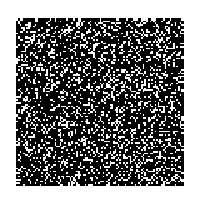
\includegraphics[width=0.9\textwidth]{game-of-life-1}
  \caption{$t = 0$}
 \end{subfigure}%
 %
 \begin{subfigure}{0.4\textwidth} \centering
  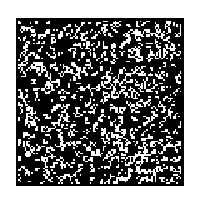
\includegraphics[width=0.9\textwidth]{game-of-life-2}
  \caption{$t = 1$}
 \end{subfigure}
 
 \begin{subfigure}{0.4\textwidth} \centering
  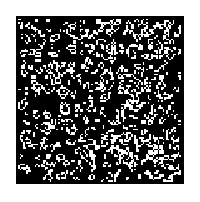
\includegraphics[width=0.9\textwidth]{game-of-life-3}
  \caption{$t = 3$}
 \end{subfigure}%
 %
 \begin{subfigure}{0.4\textwidth} \centering
  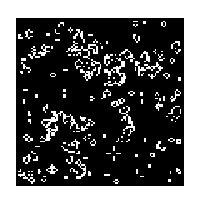
\includegraphics[width=0.9\textwidth]{game-of-life-4}
  \caption{$t = 44$}
 \end{subfigure}
 
 \caption{Několik generací výpočtu buněčného automatu \uv{Hra života} s náhodnou počáteční konfigurací} \label{img:GameOfLife}
\end{figure}

%%%%%%%%%%%%%%%%%%%%%%%%%%%%%%%%%%%%%%%%%%%%%%%%%%%%%%%%%%%%%%%%%%%%%%%%%%%%%%%
\subsection{Buněčné fuzzy automaty}
Buněčný fuzzy automat není na rozdíl od klasického fuzzy automatu prostým zobecněním bivalentního buněčného automatu. Hlavním důvodem je bezesporu fakt, že přechodová funkce bivalentního buněčného automatu je determinstická a úplná. Tedy, že každá buňka vždy přejde ze stavu $q$ do nějakého stavu $q'$. Buňka se tedy musí nacházet vždy v právě jednom stavu. Nemůže nastat situace, že by buňka přešla \uv{do více stavů současně}\footnote{Jak bude ukázáno, tento předpoklad lze obejít} (přechodová funkce by nebyla deterministická) nebo nepřešla do žádného (přechodová funkce by nebyla úplná).

Vzhledem k tomu, že stejné chování budeme vyžadovat i u buněčného fuzzy automatu, \uv{odstupňování} přechodové funkce (zavední fuzzy přechodové funkce) by nemělo smysl\footnote{Teoreticky by bylo možné nahradit stav buňky fuzzy stavem buňky. Takováto úprava by však výrazně zvýšila výpočetní šložitost výpočtu automatu a například také znesnadnila grafické znázornění jeho konfigurací a proto zde nebude uvažován.}.

Lze se tak setkat s definicí buněčného fuzzy automatu jakožto buněčného automatu pracujícího s množinou stavů rovnu intervalu $[0,1]$. Časteji bšak bývá buněčný fuzzy automat definován jako buněčný automat, jehož přechodová funkce není určena \uv{klasickými} \ifthen pravidly, ale fuzzy \ifthen pravidly.

\begin{example}
 Příkladem buněčného fuzzy automatu může být například následující automat. Množina stavů bude obsahovat přirozená čísla z intervalu $[0, 150)$. Mějme lingvistickou proměnnou $\varsigma$ a její čtyři štítky $\varsigma_L$, $\varsigma_M$, a $\varsigma_H$.
 %ve významu \uv{hodnota $q$ je nízká}, \uv{hodnota $q$ je střední} a \uv{hodnota $q$ je vysoká}. 
 Pravidla automatu pak mohou vypadat následovně:
 \begin{itemize}
  \item Pokud $q^{(t)}_{i-1,j-1} = L$, pak $q^{(t+1)}_{i,j} = H$
  \item Pokud $q^{(t)}_{i-1,j-1} = L$ nebo $q^{(t)}_{i-1,j-1} = M$, pak $q^{(t+1)}_{i,j} = M$
  \item Pokud $q^{(t)}_{i,j-1} = L$ a $q^{(t)}_{i,j+1} = L$, pak $q^{(t+1)}_{i,j} = L$
 \end{itemize}
\end{example}


\TODO{desetinná čísla s desetinnou čárkou, ne tečkou!!!!}


%%%%%%%%%%%%%%%%%%%%%%%%%%%%%%%%%%%%%%%%%%%%%%%%%%%%%%%%%%%%%%%%%%%%%%%%%%%%%%%
%%%%%%%%%%%%%%%%%%%%%%%%%%%%%%%%%%%%%%%%%%%%%%%%%%%%%%%%%%%%%%%%%%%%%%%%%%%%%%%
%%%%%%%%%%%%%%%%%%%%%%%%%%%%%%%%%%%%%%%%%%%%%%%%%%%%%%%%%%%%%%%%%%%%%%%%%%%%%%%
\section{Užitečné techniky pro práci s fuzzy automaty}

Fuzzy automaty či jim podobné modely zavedené v předchozích kapitolách jsou z pohledu pracktických aplikací pouze teoretické modely. V reálných aplikacích je často nutné pracovat s těmito modely spíše jen jako s kostrou, od které je poté odvozen výsledný model nebo algoritmus.

V této kapitole budou některé ze základních technik, jak fuzzy automaty přiblížit reálným aplikacím, odprezentovány. Demonstrovány budou na nedeterministickém fuzzy automatu, nicméně není problém aplikovat je na jakýkoliv jiný typ fuzzy automatu.

% 
% Rozpoznávání vzorů obecně je jednou z nejvýznamějších aplikací informatiky. V běžném životě se často setkáváme se situacemi, kdy je třeba v datech najít výskyt učitého vzoru, popř. jeho další vlastnosti. Případně určit podobnost ke vzoru, nebo nejpodobnější vzor.
% 
% Typickým příkladem je např. detekce obličeje na fotografii, tedy rozpoznávání vzorů v obrazových datech. Vzory je však možné rozpoznávat v téměř jakýchkoliv datech, například textech, zvukových záznamech či výsedcích měření nebo pozorování.
% 
% Z pohledu teoretické informatiky je však základem vyhledávání vzorů v textových datech. Textová data, tedy řetězce, mají jednoduchou strukturu a lze s nimi snadno manipulovat. Na druhou stranu, jsou schopna reprezentovat nebo kódovat široké spektrum dat. Právě z tohoto důvodu je studium rozpoznávání textových vzorů klíčové pro zpracovávání jakýchkoliv dalších typů dat.
% 
% \begin{note}
%  Pokud nebude uvedeno jinak, pojem \uv{rozpoznávání textových vzorů} bude v této kapitole zkracován jen na \uv{rozpoznávání vzorů}.
% \end{note}
% 
% %%%%%%%%%%%%%%%%%%%%%%%%%%%%%%%%%%%%%%%%%%%%%%%%%%%%%%%%%%%%%%%%%%%%%%%%%%%%%%%
% \subsection{Formální zavedení problému}
% Stejně tak, jak se mohou různit aplikace rozpoznávání vzorů, i samotný pojem \uv{rozpoznávání vzorů} bývá chápan různě. V nejzákladnější podobě se jedná o problém určení, zda-li pozorovaný řetězec odpovídá předem stanovenému vzoru. Vzorem bývá obvykle také řetězec, ale může jím být například regulérní výraz. Také - může nás zajímat buď exaktní shoda pozorovaného řetězce se vzorem, nebo jen nějaká forma podobnosti. 
% 
% V rozšířeném smyslu může být problém chápán jako klasifikace. Tedy, určení třídy, do které by měl pozorovaný řetězec spadat, typicky na základě podobnosti s vybrannými reprezentanty jednotlivých tříd. 
% 
% V této kapitole se však budeme zabývat pouze určováním podobnosti vzorového a pozorovaného řetězce. U každé instance problému budeme znát abecedu se kterou pracujeme a také vzor. Vzorem bude libovolný řetězec nad touto abecedou. Řešením tohoto problému pro nějaký, tzv. pozorovaný, vstupní řetězec bude úroveň podobnosti tohoto řetězce s vzorovým. Jako podobnost zde budeme uvažovat reálné číslo z intervalu $[0, 1]$, kde $0$ znamená úplnou rozdílnost a $1$ úplnou shodu. 
% 
% \begin{note}
%  Vzorový řetězec budeme v této kapitole vždy značit $\omega$, pozorovaný pak $\alpha$.
% \end{note}
% 
% Nyní máme zadefinován problém samotný, nicméně je třeba zdůraznit, že v jeho definici se používá vágní pojem \uv{podobnost řetězců}. Podobnost řetězců je totiž pojem, který souvisí s konkrétní instancí problému a nelze jej nějak přesně, ale současně dostatečně obecně popsat. Jedinné, co o podobnosti řetězců můžeme říct, je, že čím vyšší toto číslo je, tím by si měly být řetězce podobnější.
% 
% Například, budeme-li porovnávat vstup zadaný z klávesnice počítače oproti nějakému vzoru, je možné, že uživatel udělá překlep. V takovém případě bude vzorovému řetězci určitě více podobný řetězec obsahující dva překlepy (záměna symbolu za některý sousedící na klávesnici) než jiný, který se sice bude lišit jen v jednom symbolu, ale to takovém, který je na opačné straně klávesnice.
% 
% Obdobně, pokud budeme pracovat s abecedou malých a velkých písmen (majuskule a minuskule). Uvažujme vzorový řetězec \str{hello}. Řetězec \str{HELLO} se s ním neshoduje v ani jednom symbolu, ale přesto jejich podobnost může být blízká jedné.
% 
% % \begin{definition}[Problém rozpoznávání vzorů]
% %   Mějme konečnou abecedu $\Sigma$ a řetězce $\omega, \alpha \in \Sigma^*$ nad touto abecedou. Řetězec $\omega$ nazývejme \term{vzor}, řetězec $\alpha$ pak \term{pozorovaný řetězec}. Problém rozpoznávání vzorů je problém určení podobnosti řetězce $\alpha$ od řetězce $\omega$. Pokud nebude uvedeno jinak, podobnost uvažijeme jako reálné číslo z intervalu $[0, 1]$.
% % \end{definition}
% 
% %%%%%%%%%%%%%%%%%%%%%%%%%%%%%%%%%%%%%%%%%%%%%%%%%%%%%%%%%%%%%%%%%%%%%%%%%%%%%%%
% \subsection{Motivace k použití fuzzy automatů}
% Klasická teorie automatů vznikla jako nástroj pro zpracování textových řetězců. Z tohoto důvodu je rozpoznávání textových vzorů jejím základním výsledkem. Automaty obecně jsou nástroje sloužící pro rozhodování, zda-li řetězec odpovídá vzoru automatem reprezentovaném. Použití pro rozpoznávání řetězcového vzoru tak bude jen speciálním případem jejich užití.
% 
% V předchozí podkapitole jsme si stanovili, že řešením našeho problému je číslo z intervalu $[0,1]$. Z tohoto důvodu nebude možné využít klasické bivalentní automaty. Fuzzy automaty pracují se stupněm pravdivosti, který by mohl s hodnotou podobnosti řetězců korespondovat. Navíc, v praxi se často setkáme s texty, které jsou nepřesné a nedokonalé. Fuzzy přístup by nám tak mohl pomoci na tyto nepřesnosti adekvátně reagovat.
% 
% \TODO{a co pravděpodobnostní?} \TODO{Protože například: \uv{pozorovaný řetězec se se vzorovým shoduje ve stupni $x$} ale \uv{je pravděpodobnost $y$, že uživatel zadal požadovaný řetězec}}

%%%%%%%%%%%%%%%%%%%%%%%%%%%%%%%%%%%%%%%%%%%%%%%%%%%%%%%%%%%%%%%%%%%%%%%%%%%%%%%
\subsection{Fuzzy automat bivalentního automatu}
V některých situacích máme k dispozici \uv{klasický} bivalentní automat\footnote{Zde je vhodné připomenout, že automat můžeme získat například také konverzí regulérního výrazu nebo regulérní gramatiky} a potřebujeme k němu sestavit odpovídající fuzzy automat. Odpovídající ve smyslu, že řetězce, které bivalentní automat přijímá (zamítá) musí fuzzy automat přijímat ve stupni $1$ ($0$).

Uvažujme automat $A = (Q, \Sigma, \mu, I, F)$ z definice \ref{def-NedBivAut}. Pak fuzzy automat $A' = (Q, \Sigma, \mu', \sigma, \eta)$ odpovídající tomuto automatu je následující:
\begin{itemize}
 \item množina stavů $Q$ a abeceda $\Sigma$ zůstávají stejné
 \item přechodová funkce $\mu'$ je dána předpisem (pro všechny $q, q' \in Q$ a $x \in \Sigma$):
 $$
  \mu'(q, x, q') = 
    \begin{cases}
     1 & \text{ pokud $(q, x, q') \in \mu$} \\
     0 & \text{ pokud $(q, x, q') \notin \mu$}
    \end{cases}
 $$
 \item množina počátečních stavů $\sigma(q) = 1$ pro všechny stavy $q \in I$, jinak $0$
 \item množina počátečních stavů $\eta(q) = 1$ pro všechny stavy $q \in F$, jinak $0$
\end{itemize}

\TODO{je potřeba příklad?}
\TODO{rozebrat, jestli tento automat skutečně dělá to, co má? Asi by to chtělo}


%%%%%%%%%%%%%%%%%%%%%%%%%%%%%%%%%%%%%%%%%%%%%%%%%%%%%%%%%%%%%%%%%%%%%%%%%%%%%%%
\subsection{Fuzzy automat rozpoznávající $\omega$}
Další ze základních pomůcek pro práci s fuzzy automaty je automat, který v jednotkovém stupni rozpoznává pouze jeden konkrétní řetězec nad nějakou známou abecedou $\Sigma$. Tento řetězec budeme v této a některých dalších podkapitolách nazývat \uv{vzorový} a značit $\omega$.

Pro konstrukci automatu rozpoznávající řetězec omega bychom mohli použít následující postup:
\begin{enumerate} 
 \item Známe řetezec $\omega$ nad abecedou $\Sigma$
 \item Označme $L(\omega)$ jako jednoprvkový fuzzy jazyk obsahující řetězec $\omega$ ve stupni $1$
 \item Jazyk $L(\omega)$ je konečný a tudíž i regulérní. \TODO{ozdrojovat, nebo se odkázat do úvodu, platí to i pro fuzzy jazyky?}
 \item Můžeme tak k němu sestavit nedeterminstický fuzzy automat $A(\omega)$, který jazyk $L(\omega)$ rozpoznává.
\end{enumerate}

My však použujeme jinou, intuitivnější, úvahu. Automat bude v každém kroku konzumovat symboly ze vstupního řetězce a porovnávat je se symboly vzorového řetězce na odpovídajících pozicích. Pokud dojde ke shodě na všech pozicích, automat dojde do koncového stavu a sledovaný řetězec přijme. Pokud se symboly shodovat nebudou, automat nebude mít definován žádný odpovídající přechod, kterým by pokračoval ve výpočtu, a řetězec tak zamítne. Formálně pak:

\begin{definition}[Fuzzy automat rozpoznávající $\omega$] \label{def-FuzzAutRozpOme}
  Mějme řetězec $\omega$ nad abecedou $\Sigma$ délky $n$. Fuzzy automat rozpoznávající $\omega$ je pak automat $A(\omega) = ( Q, \Sigma, \mu, \sigma, \eta )$ kde
  \begin{itemize}
   \item $\sigma(q_0) = 1$ a $\sigma(q_i) = 0$ pro všechna $i > 0$
   \item $\eta(q_n) = 1$ a $\eta(q_i) = 0$ pro všechna $i < n$
   \item $\mu(q_{k}, a_k, q_{k+1}) = 
      \begin{cases}
	1		& \text{ pokud je $a_k$ $k$-tý symbol řetězce $\omega$} \\
	0		& \text{ jinak}
      \end{cases}
      $
  \end{itemize}
\end{definition}

\begin{example}
 Příklad fuzzy automatu rozpoznávající řetězec $\omega = $ \str{hello} se nachází na obrázku \ref{diag-AutRozpHell}.   

  \begin{figure}
    \includegraphics{techniques0}
    \caption{Automat rozpoznávající \str{hello}} \label{diag-AutRozpHell} 
  \end{figure}
\end{example}

%%%%%%%%%%%%%%%%%%%%%%%%%%%%%%%%%%%%%%%%%%%%%%%%%%%%%%%%%%%%%%%%%%%%%%%%%%%%%%%
% \subsection{Konstrukce fuzzy automatu z konečného automatu}
% V praxi se často setkáme z problémem, kdy máme k dispozici konečný bivalentní automat avšak my potřebujeme pro naši práci fuzzy automat. Je tedy třeba zkonstruovat takový fuzzy automat, který rozpoznává odpovídající jazyk odpovídající jazyku rozpoznávaném naším bivalentním automatem. 
% 
% Důležité je zmínit, že nelze zkonstruovat fuzzy automat, rozpoznávající stejný jazyk neboť fuzzy automat rozpoznává fuzzy jazyk, zatímco bivaletní automat klasický \uv{bivalentní} jazyk. Můžeme však sestavit automat takový, který přijímá řetězce ve stupni $0$ nebo $1$ podle toho, jestli je přijímal bivaletní automat.
% 
% Formálně řečeno, pro konečný (nedeterministický) bivalentní automat $A$ budeme konstruovat nedeterministický fuzzy automat $A'$ takový, že bude pro všechna $x \in \Sigma^*$ splněna následující rovnost:
% $$
%  \mathcal{L}(A')(\omega) = 
%   \begin{cases}
%    1 & \text{ pokud } \omega \in \mathcal{L}(A) \\
%    0 & \text{ pokud } \omega \notin \mathcal{L}(A)
%   \end{cases}
% $$
% 
% \begin{note}
%  Postup budeme provádět pro nedeterministické automaty. To jednak proto, že nedeterministické automaty jsou obecnější, než deterministické, a navíc, protože jsou v praxi využívány častěji. \TODO{ozdrojovat, klidně někde, kde rozebírám determinizmus vs. nedeterminizmus}
% \end{note}
% 
% Nyní se podíváme na to, jak výsledný fuzzy automat bude vypadat. Abeceda i množina stavů automatu zůstanou zachovány, lišit se tedy bude pouze množina počátečních a koncových stavů a přechodová funkce. \TODO{fuzzy subset $I$, $F$ a $\delta$? nebo tak něco, z teorie fuzzy množin?}
% 
% \begin{definition}[Fuzzy automat bivalentního automatu] \label{def-FuzzAutBivAut}
%   Mějme řetězec konečný nedeterministický automatu $A = ( Q, \Sigma, \delta, I, F )$. Pak nedetermintistický fuzzy automat přijímájící korespondující jazyk je automat $A' = ( Q, \Sigma, \mu, \sigma, \epsilon )$ kde pro všechna $q_i, q_j \in Q$ a $x \in \Sigma$:
%   \begin{itemize}
%    \item $\sigma(q_i) =
%     \begin{cases}
%      1 & \text{ pokud } q_i \in I \\
%      0 & \text{ pokud } q_i \notin I
%     \end{cases}$
%     
%    \item $\eta(q_i) =
%     \begin{cases}
%      1 & \text{ pokud } q_i \in F \\
%      0 & \text{ pokud } q_i \notin F
%     \end{cases}$
%     
%     \item $\mu(q_i, x, q_j) = 
%      \begin{cases}
%       1 & \text{ pokud } q_j \in \delta(q_i, x) \\
%       0 & \text{ pokud } q_j \notin \delta(q_i, x)
%      \end{cases}$
%   \end{itemize}
% \end{definition}
% 
% \TODO{rozebrat, jestli tento automat skutečně dělá to, co má? Asi by to chtělo}
% 
% \TODO{vymyslet nějaký fakt pěkný příklad}

%%%%%%%%%%%%%%%%%%%%%%%%%%%%%%%%%%%%%%%%%%%%%%%%%%%%%%%%%%%%%%%%%%%%%%%%%%%%%%%
\subsection{Podobnost symbolů}
V této a následujících podkapitolách budou popsány základní techniky, jak chování automatu upravit tak, aby více odpovídalo reálným aplikacím. Například, máme fuzzy automat, který rozpoznovává určitý fuzzy jazyk. Řetězce, které se určitým způsobem \uv{podobají} řetězcům toho jazyka, však tento jazyk obvykle obsahuje v nulovém stupni. Vzniká zde tedy snaha přizpůsobit automat tak, aby i takovéto řetězce v určitém nenulovém stupni přijímal.

Základním nástrojem, jak toho dosáhnout je pomocí podobnosti symbolů. Některé symboly mohou totiž vykazovat určitou formu podobnosti a tudiž možné zamněnitelnosti. Například znaky ASCII tabulky, které se liší v jednom bitu. Podobnost symbolů však nemusí být klasická \uv{bivalentní} relace, ale je výhodné použít fuzzy relaci. V takovém případě by podobnost znaků ASCII tabulky mohla být formulována následovně: \uv{znaky $x$ a $y$ se liší o $\delta$ bitů ve stupni $1 - \delta/8$}.

Formálně se tedy jedná o fuzzy relaci $\mathbin{\simeq}: \Sigma \times \Sigma \rightarrow [0, 1]$. Tato relace zjevně musí splňovat symetrii ($\mathbin{\simeq}(x, x) = 1$) a reflexivitu ($\mathbin{\simeq}(x, y) = \mathbin{\simeq}(y, x)$) (pro všechny $x, y \in \Sigma$).\TODO{a tranzitivita?} Fuzzy relace podobnosti symbolů pak může být součástí automatu. V takovém případě dojde ke modifikaci výpočtu automatu takovým způsobem, že ve značení \ref{not:muOverSym} a definici \ref{def-RozPreFunFuzzStav} bude nahrazen výraz $\mu(q, x, q')$ následujícím výrazem
$$
  \bigvee_{y \in \Sigma} \mu(q, y, q') \otimes \mathbin{\simeq}(x, y)
$$

Tento zápis říká, že při vstupu $x$ automat má zkontrolovat všechny ostatní symboly $y$, které by mohly být se symbolem $x$ podobné a v takovém případě realizovat přechod přes symbol $y$. Takto modifikovaný automat tak umožňuje namísto symbolu $x$ \uv{rozpoznat} jiný symbol. Můžeme tak říci, že automat umožňuje ve vstupu náhradu symbolu.

Další informace a příklady k této technice jsou k nalezení v \cite{RamGir-ConvFinAutFuzzAutStrComp}. V \cite{Ech-DefSyssConPre} je pak tato technika prezentována v mírně pozměněné formě. Symboly nahrazují tzv. fuzzy symboly, což jsou fuzzy množiny symbolů danému symbolu podobné.

% Jiným příkladem může být automat pro modelování počasí. Pro takový automat budou události \uv{jasno} a \uv{skoro jasno} velmi podobné a s lehce sníženým stupňem pravdivosti nahraditelné.


% 
% Nejzákladnější technika pro zanesení neostrého (stupňovitého) rozpoznávání je s využitím podobnostní relace symbolů. Tato technika byla přejata z . Myšlenkou této techniky je, že symbol v pozorovaném řetězci může být snadno zaměněn za jiný, podobný, jemu odpovídající v řětězci vzorovém.
% 
% Pro realizaci této techniky je potřeba mít k dispozici fuzzy relaci $s: \Sigma \times \Sigma \rightarrow [0, 1]$. Tato relace popisuje podobnost dvojice symbolů. Tedy, je-li pro nějakou dvojici symbolů $x, y \in \Sigma$  $s(x, y) = 0$, pak se jedná o naprosto rozdílné symboly. Naopak, pokud bude $s(x, y) = 1$, pak se jedná o shodné symboly. Je zjevné, že by relace $s$ měla být symetrickou a reflexivní. \TODO{v článku to nepíší, ale měla by to být relace ekvivalence (Sym, Ref, Tra). Existuje něco, jako fuzzy relace ekvivalence?}
% 
% \begin{example}
%  Jako příklad podobnostní relace (nad abecedou písmen anglické abecedy) může posloužit například vzdálenost patřičných kláves na klávesnici. V takovém případě by určitě platilo kupříkladu $s(a,s) > s(a, d) > s(a, l)$. Protože klávesy \str{A} a \str{S} jsou si blíž (a tudíž symboly $a$ a $s$ jsou si \uv{podobnější}) než například \str{A} a \str{D} či \str{A} a \str{L}.
%  
%  Jiným příkladem může být například vizuální podobnost napsaných (malých psacích) písmen. V takovém případě by zřejmě platilo $s(a, o) > s(m, t)$, protože malá psací písmena \str{a} a \str{o} jsou si vizuálně podobnější než \str{m} a \str{t}, která vypadají úplně rozdílně.
% \end{example}
% 
% Máme-li k dispozici relaci $s$, je nutné ji zakomponovat do automatu. Jak autoři uvádějí, tato technika může pracovat s libovolným konečným automatem. Podíváme se proto nejdříve, jak využít relaci $s$ obecně. Následně ji aplikujeme na automat rozpoznávající $\omega$, čímž získáme nástroj pro podobnostní rozpoznávání textového vzoru.
% 
% \begin{definition}[Automat pracující s $s$] \label{def-AutPracGS}
% Uvažujme, že máme nedeterminstický automat $A$ a relaci podobnosti symbolů $s$. Pak k automatu $A$ můžeme zkonstruovat fuzzy automat $A'$, který navíc pracuje s $s$. Takový automat bude zkonstruován dle definice \ref{def-FuzzAutBivAut} s tím rozdílem, že přechodová funkce $\mu$ bude definována pro všechna $q_i, q_j \in Q$ a $x \in \Sigma$ následovně:
% $$
%  \mu(q_i, x, q_j) = \bigvee_{y \in \Sigma} (s (x, y) \wedge \delta_y (q_i, q_j))
% $$
%  kde $\delta_x(q_i, q_j) = 
%   \begin{cases}
%    1 & \text{ pokud } q_j \in \delta(q_i, x)		\\
%    0 & \text{ pokud } q_j \notin \delta(q_i, x)
%   \end{cases}
%  $ pro všechna $q_i, q_j \in Q$ a $x \in \Sigma$.
% \end{definition}
% 
% Definice je vcelku přímočará. Pro každý přechod ze stavu $q_i$ do stavu $q_j$ přes symbol $x$, procházíme přechody původního automatu. Obsahovala-li přechodová funkce původního automatu přechod ze stavu $q_i$ přes symbol $y$ do stavu $q_j$, pak je $s (x, y) \wedge \delta_y (q_i, q_j)$ rovno podobnosti $x$ a $y$. V opačném případě je roven nule. Hodnota tohoto výrazu je díky spojení přes všechny symboly maximalizována.
% 
% Nyní aplikujeme tento způsob konstrukce fuzzy automatu na automat rozpoznávající $\omega$.
% 
% \begin{definition}[Automat rozpoznávající $\omega$ pracující s $s$]
%  Mějme abecedu $\Sigma$, řetězec $\omega$ nad touto abecedou a fuzzy relaci $s$ nad touto abecedou. Dle definice \ref{def-AutRozpOme} můžeme zkonstruovat nedeterministický bivalentní automat $A(\omega)$ rozpoznávající $\omega$. Jako automat rozpoznávající $\omega$ pracující s $s$ označme nedeterministický fuzzy automat $A'(\omega)$, který byl z automatu $A(\omega)$ vytvořen podle definice \ref{def-AutPracGS}.
% \end{definition}
% 
% \TODO{neměl by se takovýto automat místo $A'(\omega)$ značit třeba $A_{s}(\omega)$? }
% 
% Následuje jednoduchý příklad takového automatu.
% 
% \begin{example} \label{ex-AutRozpOmePodSym}
%  Mějme abecedu $\Sigma = \{ a, b, c, d \}$. Dále uvažujme relaci podobnosti symbolů $s$ takovou, že
%  \begin{itemize}
%   \item každý symbol je podobný sám sobě ve stupni $1$
%   \item každý symbol je podobný symbolu ve stupni $0,5$ jedná-li se o symboly reprezentující sousedící písmena abecedy
%   \item každý symbol je podobný symbolu ve stupni $0,3$ jedná-li se o symboly reprezentující ob-jedno písmeno sousedící písmena abecedy
%   \item všechny ostatní dvojice symbolů jsou si podobny ve stupni $0$
%  \end{itemize}
%  Tuto relaci můžeme zapsat do matice (sloupce i řádky odpovídají po řadě symbolům $a, b, c, d$):
%  $$
%  s = 
%   \begin{pmatrix}
%    1,0 	& 0,5	& 0,3	& 0,0 	\\
%    0,5	& 1,0 	& 0,5	& 0,3	\\
%    0,3	& 0,5	& 1,0 	& 0,5	\\
%    0,0 	& 0,3	& 0,5	& 1,0 	\\
%   \end{pmatrix}
%  $$
%  Nyní mějme vzorový řetězec $\omega = abc$. Pak můžeme podle předchozí definice sestavit automat $A(\omega)$ rozpoznávající $\omega$ pracující s $s$. Přechodový diagram takového automatu je na obrázku \ref{diag-AutRozpABCPracGS}.
%  
%  Tento automat evidentně rozpoznává řetězec \str{abc} ve stupni $1$. Pokud v pozorovaném řetězci nahradíme symbol \str{a} za \str{b}, bude jej automat přijímat ve stupni $0,5$. Pokud nahradíme \str{b} za \str{d}, bude jej automat přijímat ve stupni $0,3$.
%  
%  Pokud na začátek pozorovaného řetězce vložíme symbol \str{a} (tedy $\alpha = $ \str{aabc}), automat jej přijme ve stupni $0$. Stejnětak, pokud odebereme symbol \str{c} z konce vzorového řetězce (tedy $\alpha = $ \str{ab}). Pokud vložíme symbol \str{a} na začátek a současně odebereme \str{c} z konce vzorového řetězce, obdržíme pozorovaný řetězec $\alpha = $ \str{aab}. Tento řetězec bude přijat ve stupni $0,5$ \TODO{$1 \otimes 0,5 \otimes 0,5$, záleží tedy na $\otimes$}.
%  
%   \begin{figure}
%     \includegraphics{diags5}
%     \caption{Automat rozpoznávající \str{abc} pracující s $s$} \label{diag-AutRozpABCPracGS}
%   \end{figure}
% \end{example}
% 
% Z příkladu jasně vyplývá, že automat pracující s $s$ je schopen akceptovat pouze náhradu symbolu jiným symbolem. Bude-li pozorovaný řetězec oproti vzorovému obsahovat vložený symbol nebo naopak z něj bude symbol odebrán, tento typ automatu selže. Na druhou stranu jeho princip i konstrukce jsou jednoduché a snadno se s nimi pracuje.
% 
% %%%%%%%%%%%%%%%%%%%%%%%%%%%%%%%%%%%%%%%%%%%%%%%%%%%%%%%%%%%%%%%%%%%%%%%%%%%%%%%
% \subsection{Fuzzy symboly}
% Fuzzy symbol je technika využjívající podobnosti symbolů. Ve své podstatě se jedná o téže techniku jak v předchozí podkapitole, jen je na ni nahlíženo jinak. Oproti podobnosti symbolů je použití fuzzy symbolů komplikovanější, avšak umožňuje jednoduše tuto techniku kombinovat s jinými. Princip fuzzy symbolů byl přejat z \cite{Ech-DefSyssConPre}.
% 
% Mějme abecedu $\Sigma$ a relaci $p$ podobnosti symbolů (stejně jako relace $s$ v předchozí podkapitole). Fuzzy symbolem symbolu $x \in \Sigma$ označujeme fuzzy množinu symbolů takových, které jsou podle relace $p$ symbolu $x$ \uv{podobné}.
% 
% \begin{definition}[Fuzzy symbol]
% Mějme abecedu $\Sigma$ a fuzzy relaci $p \subseteq \Sigma \times \Sigma$. Pak pro každý symbol $y \in \Sigma$ definujeme fuzzy symbol $\widetilde{y}$ symbolu $y$ jako fuzzy množinu nad $\Sigma$ takovou, že pro všechna $x \in \Sigma$ platí
% $$
% \widetilde{y}(x) = p(y, x)
% $$
% \end{definition}
% 
% Vzhledem k tomu, že fuzzy symbol máme definován pro všechny $y \in \Sigma$, můžeme množinu všech takových fuzzy symbolů nazvat abecedou fuzzy symbolů.
% 
% \begin{definition}[Abeceda fuzzy symbolů]
% Mějme abecedu $\Sigma$ a fuzzy symboly $\widetilde{y}$ pro všechna $y \in \Sigma$. Pak množinu všech těchto fuzzy symbolů nazvěme abeceda fuzzy symbolů abecedy $\Sigma$ a označme $\widetilde{\Sigma}$. Tedy $\widetilde{\Sigma} = \{ \widetilde{y} \mid y \in \Sigma \}$.
% \end{definition}
% 
% Máme-li abecedu fuzzy symbolů $\widetilde{\Sigma}$, můžeme pracovat s řetězci $\widetilde{\alpha} \in \widetilde{\Sigma}^*$ nad touto abecedou. Ještě si však doplníme, jak vytvořit k řetězci $\alpha \in \Sigma^*$ jemu odpovídající řetězec fuzzy symbolů $\widetilde{\alpha} \in \widetilde{\Sigma}^*$.
% 
% \TODO{sjednotit značení $\omega$ vs. $\alpha$, když se používá jen jeden obecný řetězec}
% 
% \begin{definition}[Řetězec fuzzy symbolů]
% Mějme abecedu $\Sigma$ a nějaký řetězec $a_1 \dots a_n = \alpha \in \Sigma^*$. Pak definujme $\widetilde{\alpha} = \widetilde{a_1} \dots \widetilde{a_n}$ jako řetězec fuzzy symbolů řetězce $\alpha$.
% \end{definition}
% 
% V této fázi jsme schopni plnohodnotně pracovat s řetězci fuzzy symbolů a konstruovat je z řetězců nad abecedou $\Sigma$. Nyní přejdeme k návrhu fuzzy automatu, který bude s fuzzy symboly pracovat. Stejně jako u podobnosti symbolů i fuzzy symboly mohou být aplikovány na libovolný typ automatu. Vytvoříme proto automat pracující s fuzzy symboly nejdříve obecně, pro libovolný automat $A$. 
% 
% \begin{definition}[Automat pracující s fuzzy symboly] \label{def-AutPracFuzzSym}
%   Mějme nedeterministický fuzzy automat automat $A$. Pak fuzzy automat $\widetilde{A}$ pracující s fuzzy symboly vytvoříme tak, že v definici automatu $A$ nahradíme $\Sigma$ za $\widetilde{\Sigma}$.
%   
%   \TODO{může to tak být? a co související pojmy}
% \end{definition}
% 
% Formální zavedení automatu pracujícího s fuzzy symboly je intutivní, jedná se jen o formalitu. Abychom však využili potenciál fuzzy symbolů, je třeba pozměnit výpočet automatu. Proces jeho výpočtu se změní ve fázi výpočtu přechodové funkce fuzzy stavů. Připomeňme, že ta je definována (definice \ref{def-PreFunFuzzStav}) jako fuzzy relace $\widehat{\mu}$ přiřazující každému fuzzy stavu $V$ a fuzzy symbolu $x$ fuzzy stav dle předpisu
% $$
%  \widehat{\mu}(V, x) = V \circ \mu[x]
% $$
% 
% Zde je zjevně nutné nahradit $\mu[x]$ spojením přes všechny fuzzy symboly. Bude tedy vypadat následovně:
% $$
%  \widehat{\mu}(V, x) = V \circ \bigvee_{y \in \Sigma} (\mu[x] \wedge \widetilde{x}(y))
% $$
% 
% Tím, že je změna zakořeněna ve výpočtu automatu, nám umožňuje další práci se samotným automatem. Můžeme tedy bez problémů zkonstruovat automat rozpoznávající $\omega$ pracující s fuzzy symboly.
% 
% \begin{definition}[Automat rozpoznávající $\omega$ pracující s fuzzy symboly]
%  Mějme abecedu $\Sigma$, řetězec $\omega$ nad touto abecedou a abecedu fuzzy symbolů $\widetilde{\Sigma}$. Dle definice \ref{def-FuzzAutRozpOme} můžeme zkonstruovat fuzzy automat $A(\omega)$ rozpoznávající $\omega$. Následně pak podle definice \ref{def-AutPracFuzzSym} automat $\widetilde{A}(\omega)$ rozpoznávající $\omega$ pracující s fuzzy symboly.
% \end{definition}
% 
% Postup konstrukce takovéhoto automatu je opět vcelku intuitivní. Následuje demonstrace na příkladu.
% 
% \begin{example}
%  Mějme abecedu $\Sigma$, vzorový řetězec a podobnostní relaci $p = s$ stejné jako v příkladu \ref{ex-AutRozpOmePodSym}. Na obrázku \ref{diag-AutRozpOmePraFuzSym} je zobrazen diagram automatu $\widetilde{A}(\omega)$ rozpoznávající $\omega$ pracující s fuzzy symboly.
%  
%  \begin{figure}
%     \includegraphics{diags6}
%     \caption{Automat rozpoznávající \str{abc} pracující s $s$} \label{diag-AutRozpOmePraFuzSym}
%   \end{figure}
% \end{example}
% 
% Co se týče vlastností automatů (rozpoznávajících $\omega$) pracujících s fuzzy symboly, jejich charakteristika je vesměs stejná jako u automatů pracujících s podobností symbolů. Pouze, jak již bylo zmíněno v úvodu, nezasahují do struktury automatu jako takového.

%%%%%%%%%%%%%%%%%%%%%%%%%%%%%%%%%%%%%%%%%%%%%%%%%%%%%%%%%%%%%%%%%%%%%%%%%%%%%%%
\subsection{Editační operace, deformovaný automat}
Další technikou pro modifikaci chování automatu je využití editačních operací. Tato technika byla přejata z \cite{AstGonMenGar-FuzzAutEpsMovCmpFuzzMeasBtwStrs}. Základní idea této techniky spočívá v trojici jednoduchých editačních operací, jejiž složením jsme schopni popsat požadovanou transformaci vstupu na automatem reprezentovaný vzor. \uv{Množství} transformace pak udává podobnost pozorovaného a vzorového řetězce.

Editační operace nám určují elementární (na úrovni symbolů) transformace z řetězce na jiný řetězec. Jak bylo zmíněno, tyto elementární transformace jsou tři, a to:
\begin{enumerate}
 \item vložení symbolu
 \item odstranění symbolu
 \item nahrazení symbolu jiným symbolem
\end{enumerate}

Aplikováním posloupnosti těchto operací na vstupní řetězec tak můžeme obdržet řetězec, který odpovídá vzoru a je tak automatem přijímán. Posloupnost editačních operací budeme nazývat vyrovnání řetězců.

Pracujme nyní s abecedou $\Sigma$. Editační operace budeme zapisovat jako uspořádané dvojice $(a, b) \in (\Sigma \cup \{ \epsilon \})^2 \setminus (\epsilon, \epsilon)$. Vložení symbolu $x$ značme $(\epsilon, x)$, odstranění symbolu $x$ pak $(x, \epsilon)$ a náhradu symbolu $x$ symbolem $y$ pak $(x, y)$.  Pak všechny tři posloupnosti editačních operací jsou vyrovnáním řětězce \str{ahoj} na řetězec \str{hello}:
\begin{align*}
 & (a,\epsilon), (o,e), (j,l), (\epsilon,l), (\epsilon, o) \\
 & (a, \epsilon), (h,\epsilon), (o,\epsilon), (j,\epsilon), (\epsilon,h), (\epsilon,e), (\epsilon,l), (\epsilon,l), (\epsilon,o) \\
 & (a,h), (h,e), (o,l), (j,l), (\epsilon,o) 
\end{align*}

Označme $E$ jako množinu všech editačních operací, tj. $E = (\Sigma \cup \{ \epsilon \})^2 \setminus (\epsilon, \epsilon)$. Budeme-li chtít pro každou editační operaci stanovit stupeň, v jakém má být provedena, použijeme fuzzy relaci  $P: E \rightarrow [0, 1]$. Následovat bude popis tzv. \uv{deformace} automatu, tedy procedury, která pro fuzzy relaci editačních operací $R$ a fuzzy automat $A$ zkonstruuje fuzzy automat $A'$, který editační operace reflektuje.

\begin{definition}[Deformovaný automat] \label{def-AutRozpCalL}
 Mějme binární fuzzy relaci $R: E \rightarrow [0, 1]$ a nedeterministický fuzzy automat $A = (Q, \Sigma, \mu, \sigma, \eta)$. Pak jako deformovaný automat označme nedeterministický fuzzy automat $A' = (Q, \Sigma, \mu', \sigma, \eta)$ s $\epsilon$-přechody, kde $Q$, $\Sigma$, $\sigma$ a $\eta$ zůstávají stejné a fuzzy přechodová funkce $\mu'$ je dána:
 
 \begin{align*}
  \mu' = 	& \{ (q, x, q', d) | (q, x, q', d) \in \mu \} 			& \text{(původní přechody)}	\\
    \cup 	& \{ (q, y, q, R(\epsilon, y)) | q \in Q, y \in \Sigma \} 	& \text{(vložení symbolu)}	\\
    \cup 	& \{ (q, \epsilon, q', R(x, \epsilon)) | (q, x, q', d) \in \mu \} & \text{(odstranění symbolu)}	\\
    \cup 	& \{ (q, y, q', R(x, y)) | (q, x, q', d) \in \mu \} 	& \text{(nahrazení symbolu)}\\
  \end{align*}
\end{definition}

Význam jednotlivých složek přechodové funkce (deformací) je názorně zobrazen v tabulce \ref{tbl:DefAutDef}. Příklad deformovaného automatu je na obrázku \ref{img:DefAut}. \TODO{Okomentovat ten příklad!} 

\begin{table}
 \begin{tabular}{|l|c|}
  \hline
  Editační operace 	& Deformace (nový přechod v automatu)	 \\
  \hline
  Vložení symbolu $y$ 			& \includegraphics{techniques1} \\
  \hline
  Odebrání symbolu $x$ 			& \includegraphics{techniques2} \\
  \hline
  Narazení symbolu $x$ symbolem $y$ 	& \includegraphics{techniques3} \\
  \hline
 \end{tabular}
 \caption{Deformace automatu. Černě jsou znázorněny přechody původního automatu, červeně pak nově přidané}\label{tbl:DefAutDef}
\end{table}

\begin{figure}
  \includegraphics{techniques4}
  \caption{Ukázka deformovaného automatu (červené přechody byly přidány deformací)} \label{img:DefAut}
\end{figure}
 
Je vidět, že pomocí editačních operací jsme schopni popsat libovolnou transformaci. Deformovaný automat tak může být schopen rozpoznat v nenulovém stupni jakoukoliv transformaci řetězce, který původní automat přijímal. Je také vidět, že deformovaný automat nedokáže ošetřit pokročilejší transformace, jako je vložení právě jednoho symbolu, vložení symbolu na určité pozici či nahrazení podřetězce jiným podřetězcem. Takovéto deformace automatu je zpravidla potřeba provést ručně. Další informace ohledně editačních operací a deformovaných automatů lze nalést např. v \cite{AstGonMenGar-FuzzAutEpsMovCmpFuzzMeasBtwStrs}.

%%%%%%%%%%%%%%%%%%%%%%%%%%%%%%%%%%%%%%%%%%%%%%%%%%%%%%%%%%%%%%%%%%%%%%%%%%%%%%%
\subsection{Učící se fuzzy automaty}
Učící se automat je koncept pro propojení fuzzy automatů a strojového učení. Strojové učení je moderní přístup pro řešení obtížných úkolů. Návrh či přizpůsobení výpočetního modelu, který perfektně modeluje data z reálného světa je typický takovýto úkol. Takovým modelem může být i fuzzy automat. Velmi často se můžeme setkat s tím, že navržený fuzzy automat zcela nekoresponduje se vstupními daty (a jednoduché techniky pro ošetření těchto odchylek nebyly dostatečné). 

Důležitým předpokladem pro strojové učení je velké množství vstupních, tzv. trénovacích, dat. Strojové učení totiž data obvykle zpracovává na značně nízké úrovni, takže toto nízké množství informace je třeba kompenzovat velkým množstvím vstupů.

V této kapitole bude prezentován koncept učícího se fuzzy automatu. Jedná se o všeobecný koncept techniky, jak přizpůsobit chování automatu reálným datum. Praxe ukazuje, že učící automaty tento problém dokáží velmi efektivně řešit. Setkat se s nimi můžeme např. v \cite{FuLi-ForLeaAutAutGam}, \cite{WeeFu-FormFuzAutAppModLeaSys}, \cite{GilOmlTho-EquKnoRep+}, \cite{TzaRig-StaAnaAdaFuzzConSysUsiPetrNetLeaAut}, \cite{PatMor-EdgDetTecFuzzLogCEllLeaAutFuzzImPro}, \cite{MarMeySol-HybMetGasDifModFuzCelAutImSha}, \cite{SinGha+HybrEdgDetMetFuzSetTheCelLeaAut} \cite{AstGariGonVillFar-ApprStrMatUsiDefFuzzAutLearExpr} nebo \cite{ZhiMinLan-EvoStraIndFuFiStaAu}. Vzhledem k tomu, že konkrétní výpočty, resp. algoritmy pro učení automatu bývají poměrně komplikované, spokojíme se pouze s obecným popisem principu.

Učení fuzzy automatů je obvykle založeno na tzv. shlukování. Mějme fuzzy automat $A$ rozpoznávající jazyk  $\mathcal{L}(A)$. Tento jazyk tvoří shluky. Shluk je podmnožina jazyka $\mathcal{L}(A)$, jejiž řetězce jsou si navzájem podobnější, než s řetězci ostatních shluků. Nyní si vezměme libovolný řetězec $\omega$, který do jazyka $\mathcal{L}(A)$ nepatří. Pak můžeme najít řetězec $\omega'$ z jazyka $\mathcal{L}(A)$, který je řetězci $\omega$ určitým způsobem nejpodobnější, tj. patřil by do jeho shluku. Pak můžeme automat (resp. části automatu, kterémají vliv na rozpoznávání řětězce $\omega$) upravit tak, aby tento shluk obsahoval i řetězec $\omega$.

Konkrétní techniky jsou uvedeny v literatuře. \TODO{reálný ocitovaný příklad z některého z článků}

%%%%%%%%%%%%%%%%%%%%%%%%%%%%%%%%%%%%%%%%%%%%%%%%%%%%%%%%%%%%%%%%%%%%%%%%%%%%%%%
\subsection{Fuzzy automaty a neuronové sítě}
Umělé neuronové sítě (dále jen \uv{neuronové sítě}) jsou jednou z nejzákladnějších a nejpoužívanějších technik strojového učení. Neuronové síťě jsou inspirovány zpracováním informací pomocí nervových buněk. Neuronová síť je tvořena sítí tzv. neuronů, které jsou propojeny zpravidla v rozsáhlou síť. Tato síť obsahuje spoustu parametrů a vah, které jsou nastaveny tak, aby síť řešila patřičný problém. Při výpočtu se sítí šíří tzv. vzruchy (typicky reálná čísla), které jsou neurony přepočítávány. Více o neuronových sítích je dispozici např. v \cite{FieRus-HanNeuCom}.

Způsoby, jak sestavit neuronovou síť existují dva (v praxi se však obvykle tyto přístupy kombinují). A to pomocí trénovacích dat nebo pomocí znalostní báze. Konstrukce pomocí trénovacích dat je podobná, jako v předchozí podkapitole. Tedy, že vstupní data se postupně nechávají vyhodnocovat neuronovou sítí a ta je posléze přizpůsobována. Konstrukce pomocí znalostní báze je pak založena na kódování znalostní báze (\ifthen pravidel) do vah neuronové sítě.

Bylo zjištěno, že fuzzy automat může být konvertován do neuronové sítě. Této problematice se věnují např. v \cite{DarAhmSin-AppFuzzAutTheKnBsNeuNetDevBasLeaMod}, \cite{OmlThoGil-FuzzFinStaAutCanDetEncIntRecNeuNet} \cite{BlaDelPeg-FuzzAutIndUsNeuNet}, \cite{GilOmlTho-EquKnoRep+}, \cite{OmlThoGil-RepFuzFinStaAuConRecNeuNet}, \cite{UnaKha-FuzDFinStaMachImpBasNeuFuzSys}, \cite{PedGac-LeaFuzzAut}.

V jednodušších případech se jedná pouze o neuronovou síť, která realizuje jen přechodovou funkci automatu. Tedy neurnovou síť, jejimž vstupem je fuzzy stav, ve kterém se automat nachází, a symbol na vstupu a výstupem fuzzy stav, do kterého automat přejde. Existují však i způsoby, jak pomocí neuronové sítě reprezentovat celý automat.\TODO{najít, ve kterém článku to bylo?}

Možnosti, jak takovou neuronovou síť sestavit, jsou stejné, jako při návrhu obecné neuronové sítě. Lze tedy využít jak konstrukci pomocí trénovacích dat, tak pomocí znalostní báze. Použití trénovacích dat spočívá ve vygenerování dostatečného množství kombinací fuzzy stavů a vstupních symbolů. Pomocí automatu je určen \uv{výstupní} fuzzy stav, který je spolu se vstupem předán neuronové síti k učení. Při použití znalostní báze jsou přechodová pravidla přepsána do fuzzy \ifthen pravidel, jak bylo uvedeno v kapitole \ref{subsec:FuzzEvMach}.

Stejně tak existují způsoby, jak konvertovat neuronovou síť zpět na fuzzy automat. Postup je popsán např. v \cite{BlaDelFlo-MethIndFuzzAutUsNeuNet}, \cite{BlaDelPeg-FuzzGraIntUsiNeuNet}. 

% 
% Lze však použít i konstrukce s pomocí znalostní báze. V takovém případě je třeba zformulovat If-Then pravidla síť popisující. Pro každý přechod
% $$
%  \delta((q, d), a) = (q', d')
% $$
% tedy sestavíme If-Then pravidlo
% $$
%  \text{Je-li automat ve stavu $q$ ve stupni $d$ a na vstupu je symbol $a$, pak automat přejde do stavu $q'$ ve stupni $d'$}
% $$
% Na základě této znalostní báze může být navržena neuronová síť implementující přechodovou funkci automatu.
% 
% Opačný vztah, tj. jak z neuronové sítě zpět získat fuzzy automat je popsán např. v \cite{BlaDelFlo-MethIndFuzzAutUsNeuNet}, \cite{BlaDelPeg-FuzzGraIntUsiNeuNet}. 
% 
% Poněkud elegantní způsob, jak z neuronové sítě vyextrahovat automat je popsán v \cite{BlaDelFlo-MethIndFuzzAutUsNeuNet}. Autoři uvažují neuronovou síť jako nástroj, který rozpoznává (v odstupňované pravdivosti) ($n$-dimenzionální) podprostory prostoru $(0, 1)^n$. Každou souřadnici v tomto prostoru pak rozkládají symboly abecedy automatu, tj. každému vektoru v tomto prostoru přiřazují řetězec nad abecedou automatu. Vzniklá struktura, kterou je vlastně kd-tree, pak tvoří automat.\footnote{Tímto způsobem vygenerovaný automat je automat dle definice \TODO{doplnit ten, co má ostré přechody, ale fuzzy koncové stavy}} \TODO{Zapsat to nějak aspoň trochu lidsky, je např. potřeba doplnit práci s cykly}?
% 
% 
% 

% 
% 
% 
% 
% 
% 
% 
% 


%  
% V kontextu editačních operací budeme hovořit o \uv{skutečném vstupu} a \uv{vzoru}. 
% 
% Následuje formální definice editačních operací a pojmů s nimi souvisejících. Následně přejdeme ke konstrukci automatu, který s nimi bude schopen pracovat.
% 
% \begin{definition}[Editační operace]
% Mějme abecedu $\Sigma$, uvažujme množinu $E = (\Sigma \cup \{ \epsilon \}) \times (\Sigma \cup \{ \epsilon \}) \setminus \{ (\epsilon, \epsilon) \}$. Pak každou dvojici $(x, y) = z \in E$ nazvěme editační operace. Speciálně pak, pro všechna $x, y \in \Sigma$, $(x, y) \in E$ znamená nahrazení symbolu $x$ symbolem $y$, $(x, \epsilon) \in E$ znamená odebrání symbolu $x$ a naopak $(\epsilon, y) \in E$ pak vložení symbolu $y$. Navíc jako editační operaci uvažujme i všechny dvojce $(x, x) \in E$ (pro každé $x \in \Sigma$) symbolizující \uv{žádnou editaci}.
% 
% Máme-li editační operaci $(x, y) = z \in E$, pak označme $x = z^\downarrow$ a $y = z^\uparrow$.
% \end{definition}
% 
% Editační operace jsou tedy tři a to náhrada symbolu, vložení symbolu a odebrání symbolu. Například řetězec \str{hallo} vznikl záměnou \str{e} za \str{a} v řetězci \str{hello}. Obdobně, řetězec \str{hellow} vznikl přidáním \str{w} na konec a řetězec \str{helo} odebráním (prvního nebo druhého) symbolu \str{l}.
% 
% My však obvykle očekáváme, že došlo k více, než jedné jednoduché editaci. Je proto vhodné zavést koncept mnohanásobné editace. Jednotlivé editace za sebe seřadíme do posloupnosti v pořadí, v jakém mají být postupně aplikovány, a takovouto posloupnost nazvěme vyrovnáním řetězce $\alpha$ na řetězec $\omega$.
% 
% Uvažujme nyní množinu $E$ editačních operací jako abecedu. Pak každé vyrovnání $\zeta$ řetězce $\alpha$ na řetězec $\omega$ (posloupnost $z_1 z_2 \dots z_n$ symbolů $z_1, z_2, \dots z_n \in E$), tak můžeme považovat za řetězec nad abecedou $E$.
% 
% \TODO{fakt E považovat za abecedu a $G$ za jazyk? není to zbytečná komplikace? je to tam nutné?}
% 
% Například všechny tři následující řetězce jsou vyrovnáním řetězce \str{ahoj} na řetězec \str{hello}:
% \begin{align*}
%  \zeta_1 =& (a,\epsilon) (h,h) (o, e) (j, l) (\epsilon, l) (\epsilon, o) \\
%  \zeta_2 =& (a, \epsilon) (h, \epsilon) (o, \epsilon) (j, \epsilon) (\epsilon, h) (\epsilon, e) (\epsilon, l) (\epsilon, l) (\epsilon, o) \\
%  \zeta_3 =& (a,h) (h,e) (o,l) (j,l) (\epsilon, o) 
% \end{align*}
% 
% Na tomto příkladu je vhodné si povšimnout, že obecně může existovat více než $1$ vyrovnaní mezi libovolnou dvojicí řetězců. Bude proto vhodné neuvažovat vyrovnání jednotlivá, ale množinu všech možných vyrovnání mezi dvojicí řetězců. 
% 
% Podíváme-li se nyní jen na levé části editačních operací ve vyrovnání $\zeta_1$ z předchozího příkladu, zjistíme, že jejich zřetězením získáme řetězec $\alpha$:
% $$
% (a,\epsilon)^\downarrow (h,h)^\downarrow  (o, e)^\downarrow  (j, l)^\downarrow  (\epsilon, l)^\downarrow  (\epsilon, o)^\downarrow  = ahoj
% $$
% Stejně tak, zřetězením pravých částí editačních operací v $\zeta_1$ získáme řetězec $\omega$:
% $$
% (a,\epsilon)^\uparrow (h,h)^\uparrow  (o, e)^\uparrow  (j, l)^\uparrow  (\epsilon, l)^\uparrow  (\epsilon, o)^\uparrow  = hello
% $$
% 
% Tato vlastnost nám udává, v jakém pořadí mají být editační operace aplikovány. Stejně tak nám odstaňuje nadbytečné editační operace (např. opakované přidávání a odebírání téže znaku, které by mohlo vést až k nekonečné posloupnosti editací). Proto nám tato vlastnost poslouží jako definiční pro formání zavedení vyrovnání řetězců.
% 
% \begin{definition}[Vyrovnání řetězců \cite{AstGonMenGar-FuzzAutEpsMovCmpFuzzMeasBtwStrs}]
%  Jako množinu všech vyrovnání $G(\alpha, \omega)$ řetězce $\alpha$ na řetězec $\omega$ (kde $(\epsilon, \epsilon) \neq \alpha, \omega \in \Sigma^*$) označme takovou množinu $\{ \zeta \in E^+ \mid \zeta \text{splňuje vlastnosti 1., 2. i 3.}\}$
%  \begin{enumerate}
%   \item $\zeta = z_1 z_2 \dots z_r$, $z_i \neq (\epsilon, \epsilon)$ pro všechna $i \in 1, \dots, r$,
%   \item ${z_1}^\downarrow {z_2}^\downarrow \dots {z_r}^\downarrow = \alpha$
%   \item ${z_1}^\uparrow {z_2}^\uparrow \dots {z_r}^\uparrow = \omega$
%  \end{enumerate}
% \end{definition}
% 
% V tento okamžik máme formálně zavedena vyrovnání řetězců. Můžeme tedy přejít k práci s nimi. Ukážeme si způsob, jak pomocí vyrovnání řetězců spočítat podobnost dvojice řetězců. Na základě tohoto výpočtu pak sestavíme automat, který tento výpočet bude realizovat.
% 
% Pro uřčení podobnosti na základě vyrovnání řetězců budeme potřebovat znát míry pravdivosti editačních operací. Vstupem pro výpočet podobnosti řetězců tak bude navíc binární fuzzy relace $R$ nad množinou všech editačních operací ($E$), udávající stupeň akceptovatelnosti kadždé z možných editačních operací. S touto znalostí můžeme nadefinovat relaci podobnosti řetězců, tzv. fuzzy míru dvojice řetězců $\alpha$ a $\omega$.
% 
% \TODO{Musí být $R$ reflexivní a symetrická (def. automatu to vyžaduje, ale je to nutné?). A co T-tranzitivita?} \TODO{Takové relaci se říká relace podobnosti (proximity relation)}
% 
% \begin{definition}[Fuzzy míra\cite{AstGonMenGar-FuzzAutEpsMovCmpFuzzMeasBtwStrs}]\label{def-FuzzMir}
%  Mějme binární fuzzy relaci $R$ nad $\Sigma \cup \{\epsilon\}$. Pak jako fuzzy míru mezi řetězci $\alpha, \omega \in \Sigma^*$ (značenou $S_{\Sigma, R, \otimes}$) označme fuzzy relaci danou následujícím předpisem:
%  $$
%  S_{\Sigma, R, \otimes} = 
%   \begin{cases}
%    1	&	\text{ pokud } (\alpha, \omega) = (\epsilon, \epsilon) \\
%    \max\limits_{\zeta \in G(\alpha, \omega)} (\bigotimes_{i = 1}^{|\zeta|} R(\zeta_i) )	&	\text{ pokud } (\alpha, \omega) \neq (\epsilon, \epsilon) 
%   \end{cases}
%  $$
% % kde $\bigotimes_{i = 1}^{|\zeta|} R(\zeta_i) = R(\zeta_1) \otimes R(\zeta_2) \otimes \dots \otimes R(\zeta_{|\zeta|}$ pro $zeta_1 zeta_2 \dots zeta_{|\zeta|} = \zeta \in G(\alpha, \omega)$.
% \end{definition}
% 
% Definice fuzzy míry je vcelku intuitivní. Počítá se míra všech možných vyrovnání z nichž se vybírá ta největší. Míra vyrovnání se určuje jako t-norma ze všech $R(\zeta_i)$, tedy stupňů akceptovatelnosti jednotlivých editačních operací. Navíc, míra mezi dvojicí prázdných řetězců je dodefinována jako $1$.
% 
% Označme $\mathcal{L}(\omega)$ jako fuzzy jazyk řetězců \uv{podobných} řetězci $\omega$ s podobností danou relací $R$. Takový jazyk pak můžeme nadefinovat pro  všechna $\alpha \in \Sigma^*$ následujícím předpisem
% $$
%  \mathcal{L}(\omega)(\alpha) = S_{\Sigma, R, \otimes}(\alpha, \omega)
% $$
% 
% Nyní zkonstruujeme nedeterministický fuzzy automat s $\epsilon$-přechody, který jazyk $\mathcal{L}$ rozpoznává. 
% \TODO{rozpoznává vs. přijímá, pozor na to}
% 
% \begin{definition}[Automat rozpoznávající $\mathcal{L}$ \cite{AstGonMenGar-FuzzAutEpsMovCmpFuzzMeasBtwStrs}] \label{def-AutRozpCalL}
%  Mějme binární fuzzy relaci $R$ nad $\Sigma \cup \{\epsilon\}$ (stejná jako v definici \ref{def-FuzzMir}). Pak pro vzorový řetězec $a_1 a_2 \dots a_n = \omega \in \Sigma^*$ označme $M_{\Sigma, R, \otimes}(\omega)$ automat rozpoznávající jazyk $\mathcal{L}(\omega)$ dle definice \ref{def-NedFuzzAutEpsPre}, takový, že
%  \begin{enumerate}
%   \item množina stavů $Q = \{ q_0, q_1, \dots q_n \}$
%  % \item $\Sigma$ automatu je stejná jako $\Sigma$ v parametru
%   \item fuzzy přechodová funkce $\mu$ pro všechny $x \in \Sigma$:
%   \begin{enumerate}
%    \item $\mu(q_i, q_i, x) = R(x, \epsilon)$ pro všechny $q_i \in Q$ taková, že $i = 0, \dots, n$
%    \item $\mu(q_i, q_{i+1}, x) = R(x, a_{i+1})$ pro všechny $q_i, q_{i+1} \in Q$ taková, že $i = 0, \dots, n-1$
%    \item $\mu(q, q', x) = 0$ pro všechny $q, q' \in Q$ nesplňující předchozí dva body
% 
%    \item $\mu(q_i, q_i, \epsilon) = 1$ pro všechny $q_i \in Q$ taková, že $i = 0, \dots, n$
%    \item $\mu(q_i, q_{i+1}, \epsilon) = R(\epsilon, a_{i+1})$ pro všechny $q_i \in Q$ taková, že $i = 0, \dots, n-1$
%    \item $\mu(q, q', \epsilon) = 0$ pro všechny $q, q' \in Q$ nesplňující předchozí dva body 
%   \end{enumerate}
%   \item množina počátečních stavů $\sigma$: $\sigma(q_0) = 1$ a pro všechny ostatní $q_0 \neq q' \in Q$: $\sigma(q') = 0$ 
%   \item množina koncových stavů $\eta$: $\eta(q_n) = 1$ a pro všechny ostatní $q_n \neq q' \in Q$: $\eta(q') = 0$
%  \end{enumerate}
% \end{definition}
% 
% Máme nadefinován fuzzy automat rozpoznávající jazyk $\mathcal{L}(\omega)$. Bylo by však vhodné dokázat, že jazyk $\mathcal{L}(\omega)$, který tento automat rozpoznává je skutečně jazykem řetězců podobných řetězci $\omega$ s podobností danou relací $R$. Vzhledem ke složitosti důkazu tohoto tvrzení se v této práci spokojíme pouze s ilustrací na příkladu.
% \begin{theorem}\label{the-JazAutJeJazEditOper}
%  Mějme binární fuzzy relaci $R$ nad $\Sigma \cup \{\epsilon\}$ (stejná jako v definici \ref{def-FuzzMir}) a vzorový řetězec $\omega \in \Sigma^*$. Pak pro automat $M_{\Sigma, R, \otimes}(\omega)$ sestavený dle předcházející definice a fuzzy míru $S_{\Sigma, R, \otimes}$ platí následující rovnost
%  $$
%   \mathcal{L}(M_{\Sigma, R, \otimes}) = \mathcal{L}(\omega)
%  $$
% \end{theorem}
% \begin{proof}
%  Kompletní důkaz je k nalezení v \cite{AstGonMenGar-FuzzAutEpsMovCmpFuzzMeasBtwStrs}.
% \end{proof}
% 
% \TODO{sazba symbolů v matematickém módu vs. verbatim řetězce v textovém}
% 
% \begin{example} \label{ex-AutRozpCalL}
%  Uvažujme abecedu $\Sigma = \{a, b, c\}$ a vzorový řetězec $\omega = abc$. Zkonstruujeme automat, který bude akceptovat ve stupni $0.5$ náhradu symbolu $x$ symbolem s ním v abecedě sousedícím. Navíc uvažujme vložení symbolu $a$ ve stupni $0.2$ a odebrání symbolu $c$ ve stupni $0.1$. Tedy, relace $R$ bude vypadat následovně:
%  \begin{align*}
%   R = \{ 
%    & (a, a)/1, (b, b)/1, (c, c)/1, \\
%    & (b, a)/0.5, (a, b)/0.5, (c, b)/0.5, (b, c)/0.5, \\
%    & (a, \epsilon)/0.2, (\epsilon, c)/0.1 \}
%  \end{align*}
% 
%  Dle definice \ref{def-AutRozpCalL} můžeme sestavit automat $M_{\Sigma, R, \otimes}$. Jako $\otimes$ použijme produktovou t-normu. Získáme tak automat $M_{\Sigma, R, \otimes} = (Q, \Sigma, \mu, \sigma, \epsilon)$ takový, že:
%   \begin{enumerate}
%   \item $Q = \{ q_0, q_1, q_2, q_3 \}$
%   \item $\mu = \{ $
%   \begin{enumerate}
%    
%    \item $(q_0, q_0, a)/0.2, (q_1, q_1, a)/0.2, (q_2, q_2, a)/0.2, (q_3, q_3, a)/0.2),$
%    \item $(q_0, q_1, a)/1, (q_1, q_2, a)/0.5,$ \\
%    $(q_0, q_1, b)/0.5, (q_1, q_2, b)/1, (q_2, q_3, b)/0.5,$ \\
%    $(q_1, q_2, c)/0.5, (q_2, q_3, c)/1,$
%    \addtocounter{enumii}{1} %\item  \TODO{takové, jako $(q_3, q_1, a)$}
%    \item $(q_0, q_0, \epsilon)/1, (q_1, q_1, \epsilon)/1, (q_2, q_2, \epsilon)/1, (q_3, q_3, \epsilon)/1),$
%    \item $(q_2, q_3, \epsilon)/0.1$
%    \addtocounter{enumii}{1} %\item \TODO{takové, jako $(q_3, q_1, \epsilon)$}
%   \end{enumerate}
%   $ \} $ (přechody dle bodů (b) a (d) v definici jsou s nulovým stupněm a ve výpisu jsou vynechány)
%   \item $\sigma = \{ q_0/1, q_1/0, q_2/0, q_3/0  \}$
%   \item $\eta = \{ q_0/0, q_1/0, q_2/0, q_3/1  \}$
%   \\ \TODO{$\sigma = \{ x / y, ... \}$ by se mělo přepsat na $\sigma(x) = y, ...$, ne?}
%  \end{enumerate}
% 
%  Přechodový diagram tohoto automatu je k nalezení na obrázku \ref{img-AutRozpCalL}. V přechodovém diagramu jsou červeně zvárazněny pravidla pro rozpoznávání $\omega$, ostatní pravidla (doplněna dle definice) jsou černá. 
%  
%  Nyní si na pár řetězcích zkuzme ukázat platnost věty \ref{the-JazAutJeJazEditOper}. Dle definice \ref{def-RetPriAut} spočítáme stupeň, v jakém automat náš testovací rozpoznává řetězec $\alpha$:
%  \begin{align*}
%   M_{\Sigma, R, \otimes}(\alpha) 
%    =& \max_{q \in Q} (\mu^*(\sigma, \alpha)(q) \otimes \eta(q))) \\
%    =& \max\{ \mu^*(\sigma, \alpha)(q_0) \otimes \eta(q_0)), \mu^*(\sigma, \alpha)(q_1) \otimes \eta(q_1)),  \\
%     & \mu^*(\sigma, \alpha)(q_2) \otimes \eta(q_2)), \mu^*(\sigma, \alpha)(q_3) \otimes \eta(q_3)) \}   \\
%    =& \max\{ \mu^*(\sigma, \alpha)(q_0) \otimes 0), \mu^*(\sigma, \alpha)(q_1) \otimes 0),  \\
%     & \mu^*(\sigma, \alpha)(q_2) \otimes 0), \mu^*(\sigma, \alpha)(q_3) \otimes 1) \}   \\
%    =&  \mu^*(\sigma, \alpha)(q_3)
%  \end{align*}
%   
%  \begin{itemize}
%   \item řětězec $\alpha = abc$:
%   Určíme stupeň akceptance automatem:
%   $$
%   M_{\Sigma, R, \otimes}(\alpha) 
%    = \mu^*(\sigma, abc) (q_3)
%    = \widehat{\mu}(\widehat{\mu}(\widehat{\mu}(\widehat{\mu}(\sigma, \epsilon), a), b), c) (q_3)
%    = \{ q_3 / 1 \} (q_3) 
%    = 1 
%   $$
%   A následně ověříme fuzzy míru. Množina všech vyrovnání bude obsahovat například $\zeta_1 = (a,a), (b,b), (c,c)$ či 
%   $\zeta_2 = (a, \epsilon) (\epsilon, a) (b, \epsilon) (\epsilon, b) (c, \epsilon) (\epsilon, c)$. Snadno zjistíme, že $\bigotimes_{i = 1}^{|\zeta|} R(\zeta_i) $ je maximální právě pro $\zeta = \zeta_1$ a nabývá stupně $1$. A tedy $S_{\Sigma, R, \otimes}(\alpha) = 1$.
%    
%   \item řětězec $\alpha = ab$:
%   $$
%   M_{\Sigma, R, \otimes}(\alpha) 
%    = \mu^*(\sigma, ab) (q_3)
%    = \widehat{\mu}(\widehat{\mu}(\widehat{\mu}(\sigma, \epsilon), a), b) (q_3)
%    = \{ q_2 / 1, q_3 / 0.1 \} (q_3)
%    = 0,1
%   $$
%   $$
%   S_{\Sigma, R, \otimes}(\alpha) 
%    = R(a, a) \otimes R(b, b) \otimes R(\epsilon, c) 
%    = 1 \otimes 1 \otimes 0.1
%    = 0,1
%   $$
%   
%   \item řětězec $\alpha = bbb$:
%   $$
%   M_{\Sigma, R, \otimes}(\alpha) 
%    = \mu^*(\sigma, bbb) (q_3)
%    = ...
%    = \{ q_3 / 0,25 \} (q_3)
%    = 0,25
%   $$
%   $$
%   S_{\Sigma, R, \otimes}(\alpha) 
%    = R(b, a) \otimes R(b, b) \otimes R(b, c) 
%    = 0,5 \otimes 1 \otimes 0,5
%    = 0,25
%   $$
%   
%   \item řětězec $\alpha = abaca$:
%   $$
%   M_{\Sigma, R, \otimes}(\alpha) 
%    = \mu^*(\sigma, abaca) (q_3)
%    = ...
%    = \{ q_3 / 0,04 \} (q_3)
%    = 0,04
%   $$
%   $$
%   S_{\Sigma, R, \otimes}(\alpha) 
%    = R(a, a) \otimes R(b, b) \otimes R(a, \epsilon) \otimes R(c, c) \otimes R(a, \epsilon)
%    = 1 \otimes 1 \otimes 0,2 \otimes 1 \otimes 0,2
%    = 0,04
%   $$
% 
%   \item řětězec $\alpha = cba$:
%   $$
%   M_{\Sigma, R, \otimes}(\alpha) 
%    = \mu^*(\sigma, cba) (q_3)
%    = ...
%    = (\emptyset) (q_3)
%    = 0
%   $$
%   $$
%   S_{\Sigma, R, \otimes}(\alpha) 
%    = R(c, a) \otimes R(b, b) \otimes R(a, c) 
%    = 0 \otimes 1 \otimes 0
%    = 0
%   $$
%   
%   ...
%   
%  \end{itemize}
% 
%  Je tedy zjevné, že výpočet automatu $M_{\Sigma, R, \otimes}$ je v korespondenci s fuzzy mírou $S_{\Sigma, R, \otimes}$.
%  
%  \begin{figure}
%   \includegraphics{diags4}
%   \caption{Přechodový diagram automatu z příkladu \ref{ex-AutRozpCalL}} \label{img-AutRozpCalL}
%  \end{figure}
% \end{example}
% 
% Je vidět, že automat zkonstruován dle editačních operací je značně silný nástroj. Umožňuje nám velmi pohodlně popsat, jak moc mohou být konkrétní editační operace akceptovány. Editační operace vložení symbolu, náhrada symbolu a odebrání symbolu jsou pro popis modifikace vzorového řetězce přirozené.
% 
% Nevýhodou této techniky je, že jednotlivé editační operace jsou akceptovány bez ohledu na jejich výskyt v řetězci. Automat akceptuje nastanuvší editační operaci pokaždé, kde může nastat, ve stejném stupni. Často je však třeba v jiném stupni stejnou editační operaci přijímat např. na začátku a na konci řetězce pokaždé však v jiném stupni. Tento požadavek však automat zkonstruovaný pomocí editačních operací neumí zpracovat. Řešením může být například použití následující techniky.
% 
% 
% %%%%%%%%%%%%%%%%%%%%%%%%%%%%%%%%%%%%%%%%%%%%%%%%%%%%%%%%%%%%%%%%%%%%%%%%%%%%%%%
% \subsection{Deformovaný automat}
% Dalším ze způsobů, jak přijímat řetězec podobný vzorovému je s využitím deformovaného (fuzzy) automatu. Tato technika využívá tzv. deformovaného automatu, neboli automatu který byl stanoveným způsobem upraven, neboli deformován. Tato technika byla přejata z \cite{AstGariGonVillFar-ApprStrMatUsiDefFuzzAutLearExpr}.
% 
% Jako deformace může být použita prakticky jakákoliv úprava automatu. Mějme fuzzy automat $A$. Provedením deformace $x$ získáme deformovaný automat $A'$, který rozpoznává jiný jazyk, než automat $A$. Mezi nejzákladnější tři deformace patří náhrada symbolu, vložení symbolu před symbol a odebrání symbolu. Možných deformací existuje nekonečně mnoho. Mezi další deformace může patřit například (pro nějaké $x, y, z \in \Sigma$ a $i \geq 0$): \uv{náhrada symbolu $x$ na $i$-té pozici symboly $yz$}, \uv{odebrání všech výskytů symbolu $x$, které se nachází před symbolem $y$} nebo \uv{vložení sudého počtu symbolů $y$ mezi symboly $x$ a $z$}.
% 
% Provedeme-li deformaci fuzzy automatu rozpoznávající $\omega$, můžeme se na trojici základních deformací podívat konkrétně. Ukázka toho, jak by vypadal deformovaný automat po provedení jedné ze základních deformací je vyobrazeno v tabulce \ref{tbl-DefAutDef}.
% 
% \begin{table}[h]
%  \begin{tabular}{|l|l|}
%   \hline
%   Deformace	& Význam deformace	 \\
%   \hline
%   \textsc{Náhrada} symbolu na $i$-té pozici (symbolu $x$) symbolem $y$ & \includegraphics{diags1} \\	  
%     $\delta' = \delta \cup \{ (q_i, y, q_{i+1}) \}$, $Q' = Q$	&	\\
%   \textsc{Vložení} symbolu $y$ na $i$-tou pozici (před symbol $x$) & \includegraphics{diags2} \\
%     $\delta' = \delta \setminus \{ (q_i, x, q_{i+1} ) \} \cup \{ (q_i, \epsilon, q'_i), (q_i, y, q'_i), (q'_i, x, q_{i+1}) \}$, $Q' = Q \cup \{ q'_i \}$	 & \\
%   \textsc{Odebrání} symbolu z $i$-té pozice (symbolu $x$) & \includegraphics{diags3} \\
%     $\delta' = \delta \cup (q_i, \epsilon, q_{i+1})$, $Q' = Q$	 & \\
%   \hline
%  \end{tabular}
%  \caption{Deformace deformovaného automatu}\label{tbl-DefAutDef}
%  \TODO{pozor, toto je pro konečné automaty, ne pro fuzzy automaty!}
% \end{table}
% 
% Je vidět, že deformace mohou být účinným nástrojem pro rozpoznávání modifikovaných pozorovaných řetězců. Na druhou stranu, deformování automatu vyžaduje znalost fungování automatů. Často také může nastat situace, kdy výsledný zdeformovaný automat bude více, než deformovaný automat rozpoznávající $\omega$, automatem reprezentující samostatný netriviální vzor.

% \subsection{Shrnutí}
% V této kapitole byl zaveden pojem rozpoznávání textových vzorů. Bylo ukázáno, že pro klasickou teorii automatů je to triviální problém, který však kvůli nepřesnostem reálných dat vyžaduje nasazení fuzzy automatů. Bylo představeno několik technik, které pomocí fuzzy automatů umožňují přijímání řetězců podobných vzorovému. 
% 
% Nejjednodušší z nich, využívající relaci podobnosti symbolů, je vhodná na prosté nahrazování podobných symbolů. Technika fuzzy symbolů funguje na stejném principu, jen se liší ve formálním zavedení. Technika s využitím editačních operací umožňuje specifikovat stupeň akceptance základních editačních operací (vložení symbolu, odebrání symbolu, náhrada symbolu). Poslední technika, deformovaný automat, umožňuje libovolnou transformaci automatu, vedoucí až k libovolnému vzoru.

% 
% \subsection{Strojové učení}
% 
% Strojové učení je technika pro přibližné řešení komplikovaných či složitých problémů. Spočívá v tom, že namísto přímého hledání algoritmu, který požadovaný problém řeší, navrhujeme algoritmus, jehož vstupem je popis problému (ve vhodném formátu) a výstupem je algoritmus pro řešení problému. Pro popis problému se typicky používá deklarativní přístup, tj. \uv{co má být při určitém vstupu výsledkem} namísto \uv{jak ze vstupu spočítat výsledek}.
% 
% Je třeba mít na paměti, že správnost \uv{vygenerovaného algoritmu} závisí na správnosti popisu řešeného problému. Vzhledem k tomu, že strojové učení se používá pro komplikované problémy, popis problému vkládaný do patřičné techniky strojového učení bude zřejmě zjednodušený. Tím vzniká prostor pro nepřesnost řešení.
% 
% Na druhou stranu, s použitím fuzzy či pravděpodobnostního přístupu můžeme tento fakt vzít v potaz. Vygenerovaný algoritmus tak sice nebude fungovat správně, nicméně jeho výsledkem bude moci být například \uv{$y$ je správným řešením s pravděpodobností $p$} či \uv{$z$ je správným řešením ve stupni $d$}. Propojení strojového učení s fuzzy nebo pravděpodobnostního přístupu by tak mělo být přínosem. Navíc, jak bude ukázáno, může být i přirozené.
% 
% Mezi nejznáměnšjí techniky strojového učení patří například neuronové sítě, rozhodovací stromy či shlukování. Následuje popis neuronových sítí. Ty mají totiž nejlepší předpoklady pro provázání s fuzzy automaty a následné využití v praxi.

%%%%%%%%%%%%%%%%%%%%%%%%%%%%%%%%%%%%%%%%%%%%%%%%%%%%%%%%%%%%%%%%%%%%%%%%%%%%%%%
% \subsection{Neuronové sítě}
% Umělé neuronové sítě (dále jen \uv{neuronové sítě}) jsou jednou z nejzákladnějších technik strojového učení. Neuronové síťě jsou inspirovány zpracováním informací pomocí nervových buněk známých z biologie. Vygenerovaný algoritmus je tvořen sítí tzv. neuronů, které jsou propojeny v zpravidla rozsáhlou síť. Tato síť obsahuje spoustu parametrů, které jsou nastaveny tak, aby síť tvořila algoritmus řešící požadovaný problém. 
% 
% Následuje formální zavedení uvedených pojmů. Popis neuronových sítí je převzat z \cite{FieRus-HanNeuCom}. Označme $X$ jako tzv. signální množinu, tj. množinu všech možných hodnot, kterých mohou nabýt signály přešenášené prostřednictvím spojení. Dále označme $S$ jako množinu stavů neuronů. 
% 
% V tomto textu budeme jako signální množinu $X$ pokládat reálný interval $(0, 1)$ (v souladu s fuzzy teorií), jako množinu $S$ stavů pak množinu všech reálných čísel. Dále budeme uvažovat pouze neurony diskrétní (v čase). Říkáme, že diskrétní neuron $s$ nabývá v čase $t \in \mathbb{N}$ stavu $s(t)$. Dále označnme $y(t)$ jako výstup neuronu $s$ v čase $t$.
% 
% \begin{definition}[Diskrétní neuron]
%  Jako diskrétní neuron označujeme dvojici funkcí $f: X^n \times S \rightarrow S$ (přechodová funkce) a $g: S \rightarrow X$ (výstupní funkce) tak, že:
%  \begin{align*}
%   s(t) &= f(x_1(t - 1), \dots x_n(t - 1), s(t - 1)) \\
%   y(t) &= g(s(t))
%  \end{align*}
% \end{definition}
% 
% \begin{note}
%  $x_1$, ..., $x_n$ v předchozí definici značí signální spojení, a to buď ze vstupů sítě k neuronům, nebo mezi jednotlivými neurony.
% \end{note}
% 
% \begin{example}
%  Pro jeden z nejznáměnších, tzv. McCulloch-Pittsův neuron, vypadají funkce $f_j$ a $g_j$ neuronu $s_j$ následovně:
%  \begin{align*}
%   f_j(x_{1,j}(t), \dots x_{n,j}(t), s_j) &=  \sum_{i=1}^n w_{i,j} x_{i,j}(t) \\
%   g_j(x) &= 
%    \begin{dcases}
%     0 & \text{ pokud $x < \theta_j$} \\
%     1 & \text{ pokud $x \geq \theta_j$}
%    \end{dcases}
%  \end{align*}
%  kde $w_{1,j}, \dots, w_{n,j}$ jsou tzv. synaptické váhy neuronu $s_j$ a $\theta_j$ je jeho tzv. prahová hodnota. 
% \end{example}
% 
% \begin{definition}[Neuronová síť]
%  Jako neuronovou síť označme strukturu $(X, S, N, I, O, o)$, kde $X$ (signální množina) a  $S$ (množina stavů) byly popsány výše, $N$ je množina neuronů, $I \subseteq X^m$ je množina vstupních spojení a $O \subseteq X^n$ množina výstupních spojení a $o: N \rightarrow O$ zobrazení propojující neurony s výstupními spojeními.
% \end{definition}
% 
% \begin{definition}[Rekurentní a přímočará neuronová síť]
%  Obsahuje-li neuronová síť cyklus, tj. existuje v ní alespoň jeden neuron $s$ splňující
%  $$
%   s(t) = f(s_1(t - 1), \dots, s_2(t - 1 + k), \dots, s_n(t - 1), s(t - 1)) \\
%  $$
%  kde $k \geq 1$, pak se síť nazývá rekurentní. V opačném případě se nazývá přímočará.
% \end{definition}
% 
% \begin{example}
%  Mějme $I = \{ x_1, x_2, x_3 \}$, $I = \{ y_1, y_2, y_3 \}$ a $o(s_4) = y_1$, $o(s_6) = y_2$, $o(s_3) = y_3$. Pak pro množinu $N = \{ s_1, s_2, s_3, s_4, s_5, s_6 \}$ McCulloch-Pittsových neuronů znázorněných na obrázku \ref{img:SimplNeuNet} tvoří $(X, S, N, I, O, o)$ přímočarou neuronovou síť.
% \end{example}
% 
% \begin{figure}
%  \centering
%  \includegraphics{neurals0}
%  \caption{Ukázka neuronové sítě} \label{img:SimplNeuNet}
% \end{figure}
% 
% \subsection{Konstrukce neuronové sítě}
% Existují dva základní způsoby, jak zkonstruovat neuronovou síť. Prvním je pomocí znalostní báze a druhý pomocí trénovacích dat. Jak znalostní báze, tak trénovací data nám zde plní ůčel popisu problému, který má neuronová síť řešit. V praxi se často používá kombinace obou přístupů.
% 
% Uvažujme, že máme Množinu $P$ If-Then pravidel \uv{Jestliže $x_{j,1}, \dots, x_{j,n}$ pak $y_j$ }. Pak pro tuto množinu můžeme vytvořit neuronovou síť tak, že každému pravidlu $j$ vytvoříme následující neuron: \TODO{doplnit pravidlo pro disjunkce, tj. když je více pravidel s \uv{pak $y$}}
% $$
%   y_j(t) = s_j(t) = x_{j,1}(t - 1) \wedge \dots \wedge x_{j,n}(t - 1)
% $$
% 
% Takto vytvořená neuronová síť bude schopna pracovat jak s klasickými If-Then pravidly, tak i s fuzzy If-Then pravidly.
% 
% Druhým způsobem, jak zkonstruovat neuronovou síť, je pomocí trénovacích dat. Tato technika se dále dělí na učení s učitelem a učení bez učitele. V tomto textu se spokojíme s popisem učení s učitelem.
% 
% Hovoříme-li o trénovacích datech v souvislosti s učením s učitelem, pak jako trénovací data považujeme konečné zobrazení, které vstupům problému přiřazuje správné nebo očekávané výsledky. Na počátku se sestaví neuronová síť s náhodnými parametry a tzv. učení se její parametry postupně modifikují tak, aby byla schopna správně přiřazovat vstupům z trénovací množiny odpovídající výstupy.
% 
% \TODO{backpropagation algorithm (běžný algoritmus učení)?}
% 
% V praxi je možné oba přístupy kombinovat. Typicky se tedy sestaví neuronová síť pomocí znalostní báze, která je následně pomocí trénovacích dat přizpůsobena skutečným datům. Navíc, díky znalostní bázi neuronová síť je hned má hned v prvních fázích učení určitý přehled o řešeném problému a její učení tak může probíhat značně efektivněji. \TODO{fakt?}
% 
% \subsection{Fuzzy automaty a neuronovky}
% Bylo zjištěno, že fuzzy automat může být konvertován do neuronové sítě. Této problematice se věnují např. v \cite{DarAhmSin-AppFuzzAutTheKnBsNeuNetDevBasLeaMod}, \cite{OmlThoGil-FuzzFinStaAutCanDetEncIntRecNeuNet} \cite{BlaDelPeg-FuzzAutIndUsNeuNet}, \cite{GilOmlTho-EquKnoRep+}, \cite{OmlThoGil-RepFuzFinStaAuConRecNeuNet}, \cite{UnaKha-FuzDFinStaMachImpBasNeuFuzSys}, \cite{PedGac-LeaFuzzAut}.
% 
% Ve zjednodušené podobě se bude jednat o neuronovou síť, která bude realizovat jen přechodovou funkci, tj. přechod mezi stavy na základě vstupu. Vstupem neuronové sítě bude zakódování fuzzy stavu, v jakém se automat nachází a symbol na vstupu automatu. Výsledkem výpočtu pak bude informace, do jakého/jakých stavů by měl automat přejít, tj. opět fuzzy stav.
% 
% Na základě neuronové sítě realizující přechodovou funkci pak může být sestavena neuronová síť, která si sama pamatuje fuzzy stav, v jakém se výpočet nachází. Vzhledem k tomu, že taková neuronová síť bude muset být rekurentní, bude její struktura složitější a nad rámec této práce. Vstupem takové neuronové sítě pak bude v jednotlivých časových kvantech vstupní symboly a na výstupu číslo z intervalu $(0, 1)$ reprezentující stupeň, v jakém je zadaný řetězec automatem přijímán.
% 
% Sestavíme-li neuronovou síť pomocí přechodové funkce $\mu$ nám známého automatu $A$ budeme  generovat dvojice $(((q, d), a), (q', d')) \in \mu^*$ \TODO{je to tak?} tj. \uv{je-li automat ve stavu $q$ ve stupni $d$ a na vstupu je symbol $a$, pak přejde do stavu $q'$ ve stupni $d'$}. Například v \cite{BlaDelPeg-FuzzAutIndUsNeuNet} autoři demonstrují učení na automatu o dvou stavech a nad dvojprvkovou abecedou. Již po $5$ trénovacích dvojících se síť naučila rozpoznávat s $95\%$ přesností a po $432$ pokusech rozpoznávala se $100\%$ přesností (při toleranci stupně pravdivosti $1.25 . 10^{-7}$).
% 
% Lze však použít i konstrukce s pomocí znalostní báze. V takovém případě je třeba zformulovat If-Then pravidla síť popisující. Pro každý přechod
% $$
%  \delta((q, d), a) = (q', d')
% $$
% tedy sestavíme If-Then pravidlo
% $$
%  \text{Je-li automat ve stavu $q$ ve stupni $d$ a na vstupu je symbol $a$, pak automat přejde do stavu $q'$ ve stupni $d'$}
% $$
% Na základě této znalostní báze může být navržena neuronová síť implementující přechodovou funkci automatu.
% 
% Opačný vztah, tj. jak z neuronové sítě zpět získat fuzzy automat je popsán např. v \cite{BlaDelFlo-MethIndFuzzAutUsNeuNet}, \cite{BlaDelPeg-FuzzGraIntUsiNeuNet}. 
% 
% Poněkud elegantní způsob, jak z neuronové sítě vyextrahovat automat je popsán v \cite{BlaDelFlo-MethIndFuzzAutUsNeuNet}. Autoři uvažují neuronovou síť jako nástroj, který rozpoznává (v odstupňované pravdivosti) ($n$-dimenzionální) podprostory prostoru $(0, 1)^n$. Každou souřadnici v tomto prostoru pak rozkládají symboly abecedy automatu, tj. každému vektoru v tomto prostoru přiřazují řetězec nad abecedou automatu. Vzniklá struktura, kterou je vlastně kd-tree, pak tvoří automat.\footnote{Tímto způsobem vygenerovaný automat je automat dle definice \TODO{doplnit ten, co má ostré přechody, ale fuzzy koncové stavy}} \TODO{Zapsat to nějak aspoň trochu lidsky, je např. potřeba doplnit práci s cykly}?
% 

%%%%%%%%%%%%%%%%%%%%%%%%%%%%%%%%%%%%%%%%%%%%%%%%%%%%%%%%%%%%%%%%%%%%%%%%%%%%%%%
% \subsection{Učící se fuzzy automaty}
% 
% V předchozích kapitolách byly prezentovány techniky, jak konvertovat fuzzy automat na neuronovou síť a zpět. Konverzí automatu na neuronovou síť obdržíme nástroj, který nám umožňuje učení, tj. adaptaci modelu na jiná data. Zpětnou extrakcí automatu tak můžem obdržet automat, který rozpoznává jiný jazyk, a to jazyk který odpovídá trénovacím datům.
% 
% Tento postum lze však s určitou újmou na obecnosti zjedodušit. Namísto konverze automatu na neuronovou síť, její modifikaci a následnou konverzi zpět, je možné automat modifikovat napřímo. Této technice se říká učící se automat. Této technice se věnují např. v \cite{FuLi-ForLeaAutAutGam}, \cite{WeeFu-FormFuzAutAppModLeaSys}, \cite{GilOmlTho-EquKnoRep+}, \cite{TzaRig-StaAnaAdaFuzzConSysUsiPetrNetLeaAut}. V \cite{PatMor-EdgDetTecFuzzLogCEllLeaAutFuzzImPro}, \cite{MarMeySol-HybMetGasDifModFuzCelAutImSha} a \cite{SinGha+HybrEdgDetMetFuzSetTheCelLeaAut} je použit buněčný fuzzy učící se automat. V \cite{AstGariGonVillFar-ApprStrMatUsiDefFuzzAutLearExpr} používají pro učení pokročilejší techniku založenou na genetických algoritmech. Obdobně, v \cite{ZhiMinLan-EvoStraIndFuFiStaAu} učením generují kompletně nový automat (tedy přeučením náhodného).
% 
% Základní myšlenka techniky učících se automatů je obvykle, že jednotlivé stupně pravdivosti, které figurují v instanci automatu, mohou být pozměněny. V rozšířené podobě je pak možné automat rozšiřovat o kompleně nové stavy a přechody.


%%%%%%%%%%%%%%%%%%%%%%%%%%%%%%%%%%%%%%%%%%%%%%%%%%%%%%%%%%%%%%%%%%%%%%%%%%%%%%%
%%%%%%%%%%%%%%%%%%%%%%%%%%%%%%%%%%%%%%%%%%%%%%%%%%%%%%%%%%%%%%%%%%%%%%%%%%%%%%%
%%%%%%%%%%%%%%%%%%%%%%%%%%%%%%%%%%%%%%%%%%%%%%%%%%%%%%%%%%%%%%%%%%%%%%%%%%%%%%%
\section{Obecně k rozpoznávání}

%%%%%%%%%%%%%%%%%%%%%%%%%%%%%%%%%%%%%%%%%%%%%%%%%%%%%%%%%%%%%%%%%%%%%%%%%%%%%%%
\subsection{Detekce úplných $m$-árních stromů}
Základní technikou, jak lze využít fuzzy tree automaty je přímo práce se stromy. Ukážeme si, že s pomocí fuzzy tree automatů lze snadno rozpoznávat úplné $m$-ární stromy. 

\begin{definition}[Úplný strom]
 Úplný $m$-ární strom je takový strom, jehož každý uzel má buďto právě $m$ potomků (vnitřní uzly) a nebo $0$ (listové uzly).
\end{definition}

Vlastnost \uv{být úplným $m$-árním stromem} lze poměrně jednoduše fuzzyfikovat. Pro každý vnitřní uzel $v$ o $n$ potomcích určeme míru jeho úplnosti. Jinými slovy stupeň pravdivosti výroku \uv{uzel $v$ má $m$ potomků}. Tuto míru označme $\alpha_i$ a můžeme ji určit následujícím vztahem
$$
  \alpha_v = \frac{n}{m}
$$

Pro strom $t$ tvořený nelistovým uzlem $v$ pak můžeme stupeň $\alpha_t$ pravdivosti výroku \uv{$t$ je $m$-ární úplný strom} stanovit jako minimum pravdivosti výroku \uv{uzel $n$ má $m$-potomků} a pravivosti \uv{strom $t'$ je $m$-ární úplný strom} pro všechny jeho podstromy $t' \in t$.

Všechny atomické stromy tuto vlastnost splňují ve stupni $1$. Můžeme tak napsat:
$$
  \alpha_t = 
    \begin{dcases}
      1 				& \text{ pokud je $t$ tvořen listovým uzlem} \\
      \alpha_v \wedge \bigwedge_{t' \in t} \alpha_{t'} 	& \text{ pokud je $t$ tvořen nelistovým uzlem $v$}
    \end{dcases}
$$

Nyí je třeba vyjádřit tento problém v terminologii fuzzy tree automatů. Uvažujme, že strom $t$ je tvořen vnitřními uzly $I$ a listovými uzly $o$. Pak fuzzy jazyk $m$-árních úplných stromů bude fuzzy jazyk stromů nad $D_{(N,T)}$, kde $N = \{ I \}$ a $T = \{ o \}$. Zbývá tedy navrhnout fuzzy tree automat, který takový jazyk bude rozpoznávat.

Automat bude mít jeden stav $Q = \{ q_1 \}$ a přechodovou funkci $\mu_o(q_1) = 1$ a 
$$
  \mu_I(w, q_1) = \frac{|w|}{m}
$$
pro všechna $w \in \{ {q_1}^i |  1 \leq i \leq m \}$. Množina koncových stavů $F$ bude rovna $\{ q_1 \}$.

Dokážeme nyní, že automat $A = (Q, N, T, \mu, F)$ rozpoznává fuzzy jazyk úplných $m$-árních stromů. 

\begin{theorem}
 Fuzzy tree automat $A = (Q, N, T, \mu, F)$, kde $Q$, $N$, $T$, $\mu$ a $F$ jsou popsány výše, rozpoznává fuzzy jazyk úplných $m$-árních stromů.
\end{theorem}
\begin{proof}
 Jazyk automatu $A$ je roven $L(A) = \left\{ (t, c) | c = \mu_t(q_1) \right\}$ (automat $A$ má jen jeden koncový stav). Hodnota $\mu_t(q_1)$ záleží na tom, zda-li je $t$ tvořen listovým uzlem nebo ne.

 Je-li $t$ tvořen listovým uzlem $o$, tj. $t = o$, pak $\mu_t = \mu_o = 1$.
  
 Strom $t$ je tvořen vnitřním uzlem $v$ a $p(t) = I(p(t_1) \dots p(t_k))$. Existuje jedno jediné $w \in \mathcal{Q}$ takové, že $|w| = k$: $w = {q_1}^k$. Pak $\mu_t = \mu_I(w, q_1) \wedge \bigwedge_{j=1}^{k} \mu_{t_j}(q_1)$. Protože $q \in Q$ a $Q = \{ q_1 \}$, pak $\mu_I(w, q) = \mu_I(w, q_1) = \frac{k}{m} = \alpha_v$. $\bigwedge_{j = 1}^{k} \mu_{t_j}(q_1)$ je infimum přes všech $k$ podstromů stromu $t$, takže $\bigwedge_{t' \in t} \mu_{t'}(q_1)$.
  
 Předpokládejme, že platí $\mu_t(q_1) = \alpha_t$ pro všechny atomické stromy $t = a$, kde $a \in T$. Pak $\mu_t(q_1) = \alpha_v \wedge \bigwedge_{t' \in t} \mu_{t'}(q_1) = \alpha_v \wedge \bigwedge_{t' \in t} \alpha_{t'} = \alpha_t$ pro všechny stromy $t$ tvořené vnitřními uzly. Pak tedy $\mu_t(q_1) = \alpha_t$ pro všechny $t \in D_{(N, T)}$.
\end{proof}

Soubory automatu a ukázkových vstupních stromů jsou k nalezení v adresáři \impl{fuzzy-tree-automata}{m-ary-trees}.


%%%%%%%%%%%%%%%%%%%%%%%%%%%%%%%%%%%%%%%%%%%%%%%%%%%%%%%%%%%%%%%%%%%%%%%%%%%%%%%
\subsection{Lexikální analyzátor}


V \cite{MatSalSalYu-LexAnaSimFinFuzAutMod} definují fuzzy lexikální analyzátor. Funguje na bázi klasickýho pattern matching, jen s informací, ve kterém koncovém stavu zkončil.\TODO{mimochodem, v \cite{MatSalSalYu-LexAnaSimFinFuzAutMod} je poměrně pěkně popsaná teorie (determinsitické a nedeterministické automaty, regexy i reg. jazyky).}


\subsection{Rozpoznávní ručně psaného textu}
\cite{AstGariGonVillFar-ApprStrMatUsiDefFuzzAutLearExpr}, \cite{WeeFu-FormFuzAutAppModLeaSys} a podob.
...

\subsection{Detekce překlepů}
\cite{AndAbdAsm-ApprPattMatcFuzzLog} až na konci,  Fuzzy Aho-Corasick algorithm (popř. dohledat jiný zdroj).

\cite{SnaKepAbrHas-AproxStriMatchFuzzAut}

\subsection{Korekce textu pomocí pravděpodobnostních automatů}
V \cite{YorSinTis-PowAmnLeaPrAuVarMemLen} a \cite{Ron-AutLeaApp} zavádějí pravděpodobnostní automat s pamětí. Každý stav si pamatuje něco jako své prefixy. Takže je to tak trochu automat pracující s celými slovy. Spolu s učením ho používají ke korekci textu bible. A posléze pro segmentaci DNA.


\subsection{Fuzzy programy}
V \cite{Cha-ExeFuzProUsFiStaMa} popisují fuzzy programy. Fuzzy program je prakticky deklarativní program, fuzzy reguérní výraz, který popisuje, jak mají vypadat výsledky.

\subsection{Pravděpodobnost výskytu vzoru v řetězci}
V \cite{Mar+-ProAriAutApp} a \cite{Her-ProAriAutAppSoComFraBioSeqAna} používají aritmetický automat (automat, který v každém přechodu může něco udělat) pro počítání počtu výskytů vzoru v řetězci. To pak využívají na určování proteinů (protein je rozštěpen a jednotlivé peptidy jsou pomocí hmotnostního spektrometru analyzovány a hmotnosti předány automatu). 

%%%%%%%%%%%%%%%%%%%%%%%%%%%%%%%%%%%%%%%%%%%%%%%%%%%%%%%%%%%%%%%%%%%%%%%%%%%%%%%
\subsection{A dále ještě ...}
Kódování výstupu z nějakýho systému do řetězce a jeho pattern matching \cite{Rig-FauDetIsoBasFuzzAut}. 

Toto \cite{BaiTri-PattRecUsiTemFuzzAut} vypadá taky zajímavě, nějak pattern matchinguje nějaký signál či co.

V \cite{Hun-NoLiTexSeaUsFuFiStLiNoDetAut} nejspíš používají dvouúrovňový pattern matching pro vyhledávání vzoru v dlouhém textu. Nejdřív sestaví jednoduchý automat pro přibližné rozpoznání něčeho, co se vzoru podobá (ale je to jednodušší?) např. na každé stránce. Ty stránky, které prošly v nenulovém stupni pak prohledá pořádně a určí konkrétní výskyty. Asi. 

\subsection{Pravděpodobnostní rozpoznávání fonetické abecedy}
V \cite{MohPerRoe-WeiFinStaTraSpeRec} (a možná v \cite{BahJel-DecChaWinDelSubApSpeRec}) de facto překládají fonetickou abecedu na angličtinu (některá slova se totiž mohou vyslovovat  různě, např. \uv{data} a \uv{dejta} a naopak, dvě slova shodně, např. \uv{red} a \uv{red}). Z databáze sestavují automaty pro jednotlivá slova a ty na principu automatu pro lexikální analyzátor slývají do jednoho obrovského.

\subsection{Parsování MIDI ze zvuku}
V \cite{ForBel-GenMusAccUsFinStaTra} používají pravděpodobnostní automat jako jednu komponentu procesu pro parsování \uv{MIDI} dat ze zvukového záznamu.

\subsection{Reprezentace zvuků}
V \cite{OliWag-ComMusNeuNetProFiStMa} používají pravděpodobnostní automat pro reprezentaci databáze hudebních skladeb. Tj. že abeca jsou tóny a pravděpodobnosti přechodů pravděpodobnosti, v jakých se v testovacím datasetu vyskytoval za aktuálním tónem tón na vstupu automatu.



\subsection{Pattern matching přirozeného jazyka}
V \cite{WaMan-ProFiStMaRegBaMTEva} kombinují editační operace s pravděpodobnostními automaty pro pattern matching. Tentorkát však přirozeného jazyka.

\subsection{Nejpravděpodobnější řětězec}
Mějme pravděpodobnostní automat. Pak v \cite{HigOnc-ComMosProStrProFiStaMa} studují, jak najít nejpravděpodobnější řetězec, tj. řetězec s nejvyyší pravděpodobností přijetí.

\subsection{PAttern matching signálů}
V \cite{MukRay-StaSplMerProbFiStaAuSigRepAna} a ještě někde se věnují tomu, že rozkouskovat signál umožní jeho pattern matching.


\subsection{Pattern matching dvourozměrného signálu}
V \cite{Jin+-WavBasFeaExtUsPrFiStAuPatCla} je popisován způsob, jak rozpoznávat dvojrozměrný signál (mřížku signálů). Používá se k tomu model podobný pravděpodobnostním buněčným automatům. Na rozdíl od nich však tento model lépe podchycuje stavy a přechody mezi nimi na úkor větší složitosti. 

Vstupní signály jsou diskrétně kvantovány v čase a následně i v úrovni. Dále je stanoveno zobrazení, které každé buňce s daným okolím přiřadí určitý stav automatu. Pro každou buňku je poté vytvořen pravděpodobnostní automat s přechodovou funkcí ve tvaru \uv{Pravděpodobnost, že automat přejde do stavu $q''$ za předpokladu, že nyní se nachází ve stavu $q$ a na vstupu je vzorek odpovídající stavu $q'$, je rovna $p$}.

Autoři tuto techniku demonstrují na problému detekce poruch u materiálu. Měřený kus testovaného materiálu je zatěžován stále větším tlakem a postupně proměřován ultrazvukovými signály. Při namáhání materiálu dochází k jeho systematickému poškození. Změna chování materiálu je detekována ultrazvukovými senzory a předány automatu, který v nich rozpozná vznikající poruchu.

\subsection{Parsování referencí}


V \cite{Kra+-BibMeExUsiPrFiStTra} pomocí automatu parsují reference z textu a rozpoznávají v nich strukturu. Reference v textu mají totiž pevnou strukturu. Např. dle normy ČSN ISO 690:2017\TODO{ocitovat: https://sites.google.com/site/novaiso690/}:

Tvůrce. \textit{Název publikace}. Vedlejší názvy. Vydání. Další tvůrce. Místo: nakladatel, rok. Počet stran. Edice, číslo edice. ISBN.

Problém je však ten, že některé části (např. počet stran) jsou nepovinné. Dále také, např. rok vydání a počet stran jsou číselné údaje a může tak dojít ke zmatení. Běžný automat proto někdy může nalést více, než jednu shodu se vzorem. Proto používají \uv{pravděpodobnostní} (jedná se spíše o fuzzy než o pravděpdobnostní automat) automat, který dokáže určit nejbliší shodu.

\subsection{Pravděpodobnostní rozpoznávání přirozeného textu}
V \cite{KniGra-OvProTreTraNatLanPro} zpracovávají přirozený jazyk. Vzhledem k podstatě gramatiky přirozeného jazyka využívají pravděpodobnostní tree automaty. \TODO{příklad gramatického stromu}?





%%%%%%%%%%%%%%%%%%%%%%%%%%%%%%%%%%%%%%%%%%%%%%%%%%%%%%%%%%%%%%%%%%%%%%%%%%%%%%%
%%%%%%%%%%%%%%%%%%%%%%%%%%%%%%%%%%%%%%%%%%%%%%%%%%%%%%%%%%%%%%%%%%%%%%%%%%%%%%%
%%%%%%%%%%%%%%%%%%%%%%%%%%%%%%%%%%%%%%%%%%%%%%%%%%%%%%%%%%%%%%%%%%%%%%%%%%%%%%%
\section{Modelování a simulace}


%%%%%%%%%%%%%%%%%%%%%%%%%%%%%%%%%%%%%%%%%%%%%%%%%%%%%%%%%%%%%%%%%%%%%%%%%%%%%%%
\subsection{Automobilismus}
Automat (pochopitelně event-driven) pro monitoring manévrů řidiče (předjíždění, zatáčení doleva v křižovatce, pouštění chodce na přechodu, a podob.) \cite{Hul+-ManRecUsProFinStaMacFuzLog}. Pomocí fuzzzy stavových proměnných (rychlost, zrychlení, natočení volantu, blinkry ano/ne) se stanovují pravidla, např. odbočení v křižovatce: blinkr levý -- lehce doleva (volitelně) -- zpomalení (volitelně) -- velké otočení volantem doleva -- vypnutí blinkru.

V \cite{TriHei-ExpDesSeqFuzPer} např. sledují řízení auta pomocí fuzzy automatů. Popisují techniku, kdy na vstupu je proud dat z čidel, ty se fuzzyfikují (\uv{teplota je nízká}, \uv{prudce brzdí}, \uv{mírně zatáčí doleva}), patřičný automat pak rozpoznává známé vzory. Tedy podobné jako \cite{Hul+-ManRecUsProFinStaMacFuzLog}. Akorát tady namísto otáčení volantu a sešlápnutí pedálu měřili pomocí trojice akcelerometrů (pro tři osy, $x, y$ a $z$ intenzity akcelerace v patřičné ose, a to jestli je pozitivní, negativní nebo neutrální). Používají automat s výstupem, který tak může vybranné přechody hlásit (\uv{teď se jede rovně}, \uv{právě byla ostrá zatáčka doleva}). Získá se tak docela příjemný popis trasy.

V \cite{GraFod-FuzAutIntHybConSys} také popisují řídící systém, avšak zavádějí distribuovaný model.

%%%%%%%%%%%%%%%%%%%%%%%%%%%%%%%%%%%%%%%%%%%%%%%%%%%%%%%%%%%%%%%%%%%%%%%%%%%%%%%
\subsection{Sledování vytížení el. sítě}
V \cite{DucMarMar-AlgBasFiStMacFuzTrNoIntrLoaDis} používají fuzzy automaty pro sledování vytížení el. rozvodné sítě. Technika předpokládá znalost spotřebičů v síti a nástroj pro monitorování odběru el. proudu. Výstupem je pak rozpis, kdy byl jaký spotřebič zapnut a kolik odebíral energie.

Technika využívá faktu, že každý spotřebič se může nacházet v různých stavech. Například vysoušeč vlasů se může nacházet v jednom z těchto tří stavů: vypnut, fouká studený vzduch, fouká teplý vzduch. Každému takovému stavu může být být asociována konkrétní hodnota odběru el. energie.  Pokud známe výkyvy spotřeby proudu při změnách těchto stavů, můžeme spotřebiči sestavit fuzzy automat. Událostmi, které automat řídí mohou být  např. \uv{spotřeba velmi výrazně klesla}, \uv{spotřeba je konstantní} či \uv{spotřeba lehce stoupla}. 

Nyní uvažujme elektrickou síť s více spotřebiči. Předpokládejme, že v každou časovou jednotku dojde vždy pouze k jedné změně stavu jednoho spotřebiče. Pak nastane-li v síti událost $x$ (např. pokles spotřeby) \TODO{fuzzy událost? událost nastane ve stupni $d$? ještě jinak?}, pak na základě znalosti stavů všech spotřebičů můžeme určit nejpravděpodobnější přechod (tj. jaký spotřebič přešel do jakého stavu), který nastal. Sledováním sítě tak můžeme neinvazivně sledovat, které spotřebiče, kdy a jak zatěžují síť.

%%%%%%%%%%%%%%%%%%%%%%%%%%%%%%%%%%%%%%%%%%%%%%%%%%%%%%%%%%%%%%%%%%%%%%%%%%%%%%%
\subsection{Modelování emocí postav v počítačových hrách}
V \cite{AlvJoaCru-FuStMaAppEmoModEleGamCha} je použit fuzzy automat pro modelování nálady hráče ve hře šachy. Automat je tvořen čtveřicí stavů reprezentující jednotlivé \uv{elementární} nálady, konkrétně \uv{zamyšlený}, \uv{překvapený}, \uv{radostný} a \uv{rozzuřený}. Přechodová abeceda je tvořena následnujícími nastanuvšími tahy:
\begin{itemize}
 \item tah, který hráče dostal do výhody
 \item tah, který dostal hráče do nevýhody
 \item tah, po kterém se hráč octl v šachu (popř. matu)
 \item tah, kdy se nestalo nic z předchozích
\end{itemize}
Výhoda a nevýhoda, resp. stupeň v jakém platí \uv{hráč se dostal do výhody, resp. nevýhody} lze snadno spočítat jako rozdíl ohodnocení šachovnice. Ohodnocení šachovnice lze určit například jako výžený součet figur hráče dle jejich síly. Tah zakončený šachem může být nadefinován dvojstavově nebo např. jako \uv{stupeň matu}, tj. pro šach např. $0.5$, pro mat $1$ (jinak $0$).

Následně jsou navržena přechodová pravidla. Například, dostane-li se hráč v rozzuřeném stavu do výhodné pozice, přejde do radostného stavu.  Následně, pokud se v dalším tahu nestane nic zajímavého, přechází do zemyšleného stavu. Kompletní automat je k vidění na obrázku \ref{img:ChessEmosFA}.

\begin{figure}
 \centering
 \includegraphics{rest0}
 
 \caption{Automat pro modelování nálad hráče ve hře šachy. Stavy $q_F$, $q_S$, $q_H$ a $q_A$ reprezentují po řadě nálady \uv{zamyšlený}, \uv{překvapený}, \uv{radostný} a \uv{rozzuřený}. Symboly $p_{+}$ a $p_{-}$ značí přechod k výhodné, resp. nevýhodné situaci pro hráče, $c$ symbolizuje šach a $n$ tah bez žádné změny situace na šachovnici. Převzato z \cite{AlvJoaCru-FuStMaAppEmoModEleGamCha}, upraveno.}
 \label{img:ChessEmosFA}
\end{figure}

Na základě aktuálního fuzzy stavu (kombinace různých stupňů elementárních nálad) automatu je upravována mimika hráče a jeho obličej je zobrazován v počítačové hře. Ukázka některých herních situací je na obr. \ref{img:ChessEmosScreens}. Pro lepší uživatelský dojem autoři navíc implementovali plynulé přechody mezi stavy.

\begin{figure}
 \centering
 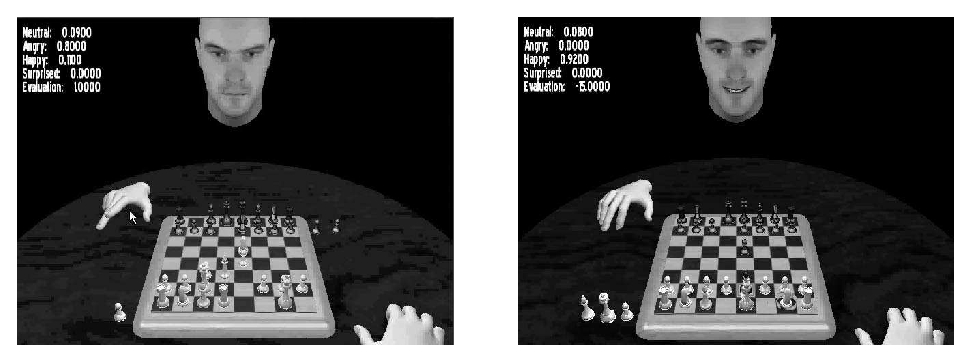
\includegraphics[width=\textwidth]{chess-emos-screens}
 
 \caption{Ukázka výrazů ve tváři hráče při ztrátě pěšce (vlevo) a při sebrání dámy (vpravo). Převzato z \cite{AlvJoaCru-FuStMaAppEmoModEleGamCha}.} \label{img:ChessEmosScreens}
\end{figure}

\TODO{zmínit v úvodech, že pokud u event automatu není uplatnitelný žádný přechod, automat zůstává ve stávajícím stavu (a neukončuje svůj výpočet, jak je obvyklé)}
\TODO{If-Then pravidla jsou prý tzv. Takagi-Sugeno-Kang pravidla (dle \cite{HeiTri-SimEmoPerHumComInt})}
\TODO{Minimálně u event-driven automatů uvést, že je vhodné nějak rozpoložit stupňě. Tedy, aby např. fuzzy stav měl v součtu vždycky $1$.}

%%%%%%%%%%%%%%%%%%%%%%%%%%%%%%%%%%%%%%%%%%%%%%%%%%%%%%%%%%%%%%%%%%%%%%%%%%%%%%%
\subsection{Modelování emocí}
V \cite{HeiTri-SimEmoPerHumComInt} je prezentován prototyp systému pro modelování lidských emocí. Systém je založen na faktu, že velký vliv na emoce člověka má počasí. V jejich modelu (pro snažší sběr dat) pak konkrétně teplota vzduchu a množství světla. Pro reprezentaci emocí používají tzv. Plutchikovo kolo emocí. Jedná se o emoční model, který reprezentuje emoce pomocí dvojice ukazatelů, aktivace a ohodnocení. Např. pozitivní aktivace a negativní ohodnocení začí odpor či opovržení, negativní aktivace při neutrálním ohodnocení znamená strach.

Autoři používají ligvistické proměnné \uv{negativní}, \uv{nutrální} a \uv{pozitivní} a jak pro aktivaci, tak pro ohodnocení. V jejich zjednodušeném modelu vstup do systému (data z teploměru a světelného čidla) nejprve transformují na odpovídající aktivaci (průměrná teplota znamená pozitivní aktivaci, nízká nebo naopak vysoká teplota pak negativní) a ohodnocení (čím je světleji, tím je ohodnocení pozitivnější).

Následně konstruují automat. Automat má 9 stavů, každé kombinaci lingvistických proměnných aktivace a ohodnocení odpovídá jeden. Poté definují přechody mezi nimi. Má-li dojít ke zvýšení (snížení, ponechání) hodnoty patřičné lingvistické proměnné, pak automat přejde k stavu odpovídajícímu vyššímu (nižšímu, stejnému) stupni této lingvistické proměnné. Například při vstupu \uv{aktivace je pozitivní a ohodnocení je neutrální} při stavu \uv{aktivace je negativní a ohodnocení pozitivní} přejde do stavu \uv{aktivace je neutrální a ohodnocení je pozitivní}. 

Z fuzzy stavu pak lze zpětně zkonstruovat, v jakém emocionálním rozpoložení se člověk aktuálně nachází. Autoři poukazují, že při pozměnění konfigurace (úprava definic fuzzy množin pro lingvistické proměnné) lze chování systému přizpůsobit povaze člověka (např. klidná povaha, pesimista a podob.), což může výsledky značně zpřesnit.


%%%%%%%%%%%%%%%%%%%%%%%%%%%%%%%%%%%%%%%%%%%%%%%%%%%%%%%%%%%%%%%%%%%%%%%%%%%%%%%
\subsection{Sledování a modelování aktivit počítačových programů}

V \cite{Maz+-ProTreAutAppBehMod} prezentují nástroj založený na pravděpodobnostních automatech, jehož úkolem je určovat nejpravděpodobnější aktivitu počítačového programu. Autoři mají k dispozici softwarový nástroj pro výpis nízkoúrovňového chování (vybraných elementárních akcí) počítačového programu (systémová volání, změny na programovém zásobníku). Sledováním těchto výpisů při známém chování programu mohou stanovit vzory chování programu. Pokud jsou tyto vzory vloženy do pravděpodobnostního automatu, je možné obdržet automat modelující chvoání programu. Lze tak například z automatu vyčíst, že pokud program otevřel soubor, pak následující elementární akcí bude s nejvyšší pravděpodobností alokace paměti na haldě.


%%%%%%%%%%%%%%%%%%%%%%%%%%%%%%%%%%%%%%%%%%%%%%%%%%%%%%%%%%%%%%%%%%%%%%%%%%%%%%%
\subsection{Sledování cen investic}
Zde \cite{ManPra-PriPatDetUsFiStMaFuzTra}, automat \uv{fuzzy-sleduje} vzory v časovém průběhu výše ceny na trhu (např. \uv{cena prudce vzrostla}). Na základě toho pak sleduje stav, v jakém stavu se cena nachází (např. těsně před výrazným růstem).

%%%%%%%%%%%%%%%%%%%%%%%%%%%%%%%%%%%%%%%%%%%%%%%%%%%%%%%%%%%%%%%%%%%%%%%%%%%%%%%
\subsection{Sledování pohybu a aktivit osoby}
V \cite{TriHei-LinSumHumActSkiConAcc} je prezentován postup, jak pomocí sledování různých parametrů (pohyb, získaný akcelerometrem, a el. vodivost kůže) určit pravděpodobnou činnost (nicnedělání, chůze, práce, odpočinek) osoby. Činnosti odpovídají stavům automatu a na základě parametrů se určijí přechody. Navíc, je pravděpodobnější, že člověk ze stavu nicnedělání přejde do stavu práce než do stavu relaxace.

Stejnou techniku využívají v \cite{Alv+-HumActRec+}. Zde však detekují činnosti: chůze, práce u sebe, hovor s kolegy, dávání si kávy, míting, a to pomocí polohy zařízení (chytrý telefon) osoby (určené triangulací Wifi sítě) a polohy těla.

Poloha těla pakl může být buď, že osoba stojí, sedí nebo jde. Tyto hodnoty jsou opět sledovány fuzzy automatem (přechody jsou realizovány na základě dat z akcelerometru, pohybového čidla, a gyroskopu (senzoru náklonu). 


%%%%%%%%%%%%%%%%%%%%%%%%%%%%%%%%%%%%%%%%%%%%%%%%%%%%%%%%%%%%%%%%%%%%%%%%%%%%%%%
\subsection{Řídící systémy, fuzzy kontroléry}
Vztah fuzzy automatů a řídících systémů pracujících na bázi ontologického řízení jsou popsány např. zde \cite{HeKinSep-DecMakFuzEnvZUsOntCon+}\cite{Gra+-ApFuStFuOuFinMaPrRecVioOntAss}\cite{GraFodDri-HybFuzBooAutOntCont}. Ontologické řídící systémy se vyznačují popisem ontologických předpokladů. Ontologické předpoklady jsou popisy stavu modelovaného systému, na jejiž základě systém provádí rozhodování. Systémy ovšem bývají často tak složité, že je nemožné zanést do znalostní báze všechny možné předpoklady. Z tohoto důvodu může u systému dojít k tzv. porušení ontologických předpokladů (např. při chybě či nečekaném vnějším podnětu). Dalo by se říci, že systém se takto dostane do nekonzistentního stavu.

Je-li systém modelován klasickým, bivalentním automatem \TODO{on ani tak není klasický bivalentní, ale event-driven} je pravděpodobné, že takovouto situaci nebude schopen ošetřit. Mohl by se tak ve snaze provést synchronizaci reálného a modelového stavu např. zacyklit mezi dvojicí diskrétních stavů.  



\subsection{Predikce průběhu hry}
V \cite{Hua+-LeaProbAutModChe} popisují, jak pomocí statistických dat sestavit automat, který něco modeluje (nastanuvší události a výsledný stav). Např., v jejich případě, skóre ve hře, jejich pravděpodobnosti a výsledný stav hry (prohra, výhra).

\subsection{Pravděpodobnostní sledování aktivit člověka}
V \cite{TurChe-MacRecHumActSur} poukazují na použití pravděpodobnostních automatů jako jednu z alternativ pro jednu z částí procesu sledování aktivit člověka pomocí automatu (podobně, jak u fuzzzy automatů výše). Uvádějí však další aplikace pro tuto techniku (biometrika, sémantická analýza videa, bezpečnost, uživatelská rozhraní, syntéza animací). 
%%%%%%%%%%%%%%%%%%%%%%%%%%%%%%%%%%%%%%%%%%%%%%%%%%%%%%%%%%%%%%%%%%%%%%%%%%%%%%%
\subsection{Problém městského růstu (urban growt problem)}
Problém městského růstu je problém z oblasti urbanistiky. Řešením tohoto problému je co nejpřesnější predikce rozvoje městské zástavby na základě historických záznamů a současné situace. Ve zobecněné podobě se nemusí jednat jen o růst městské zástavby, ale například nárust vytíženosti silnic, kácení lesů nebo vytěženost ložisk. Stejně tak se nutně nemusí jednat o růst, ale obecný vývoj v čase. V této kapitole však budeme pro jednoduchost uvažovat standardní problém, tedy městský růst.

Buněčné fuzzy automaty byly již mnohokrát použity pro řešení tohoto problému. Pomocí těchto automatů byl například modelován rozvoj zástavby v městě Riyadh v Saudské Arábii \cite{AlAhHep+-ModUrbGroDynUsCelAutGIS}, \cite{Ahm+-CalFuzCelAutModUrbDynSauAr}, regionu Helensvale v Austrálii \cite{War+-StoConCelModUrbGro}, ostrova Sv. Lucie v Krabiském moři \cite{WhiEng-CelAutBasIntDynRegMod}, oblasti North Vancover v Kanadě \cite{LaiDraSch-IntMulEvCelAutMetLanSimMod}, oblasti Mesogia v Řecku \cite{ManHatPra-FuzCelAutBasSheModUrGro+}, \cite{ManHatPra-ModUrbGroUsFuzCelAut}, oblasti Sanfranciského zálivu v Kalifornii \cite{ClaHopHay-SelModCelAutModHistUrbSanFraBayAre} nebo části Tianhe města Guangzhou v jihovýchodní Číně \cite{Wu-CalStoCelAutAppRurUrbLanConv}. %
%
Další literatura věnující se uplatnění (fuzzy) buněčných automatů při řešení problém městského růstu je k dispozici např. zde: \cite{PowSimWhi-HieFuzzPattMatcRegCompLanUseMap}, \cite{Dra-CouFuzSetTheGisBaCelAutLanUseChaMod} a \cite{LiuPhi-DevCelAutModUrbGroIncFuzSetApp}.

\TODO{el. síť \cite{WasPar-PreSpaDisEleEnCon+}? Doprava (toho mám taky povícero)? }

Pojďme se nyní podívat, jak se buněčné fuzzy automaty pro řešení tohoto problému používají. Základní idea pro nasazení fuzzy automatů je následující: Stav zástavby reprezentujme jako konfiguraci fuzzy buněčného automatu. Pak růst zástavby bude odpovídat přechodům mezi těmito konfiguracemi.

V první fázi je nutné si sledovanou oblast (\uv{město}) rozdělit na dílčí parcely. Každé takové parcele pak bude odpovídat jedna buňka buněčného fuzzy automatu. U každé parcely je třeba zjistit rozličné ukazatele, např.:
\begin{itemize}
 \item je-li parcela zastavěna (popř. jak moc)
 \item typ zástavby na parcele (např. rodinné domy, obytné domy, komerční prostory, prostory pro rekreaci, dopravní stavby, průmyslová zóna)
 \item jak moc žije na parcele obyvatel
 \item jak moc vysoké budovy stojí na parcele
 \item jak velké produkuje parcela znečištění ovzduší/hluku
\end{itemize}
Nejčastěji se jako ukazatel používá informace o zastavěnosti parcely. Ta se totiž dá poměrně snadno stanovit s pomocí satelitních snímků sledované oblasti.

Dále je třeba získat ukazatele, které mají vliv na růst zástavby. Mezi takovéto ukazatele patří například:
\begin{itemize}
 \item vzdálenost parcely od centra města (popř. škol, nákupních center, ...)
 \item dopravní obslužnost parcely (vzdálenost od hlavní silnice nebo zastávek hromadné dopravy)
 \item atraktivita lokality (výhled na město, okolní zástavba, ...)
 \item stavební podmínky (podloží, záplavová zóna, terén, ...)
\end{itemize}
Za povšimnutí stojí, že některé ukazatele jsou neměnné v čase (např. vzdálenost od centra města nebo podloží).

Následně je možné sestavit přechodová pravidla. Ta mohou být například:
\begin{itemize}
 \item Je-li vzdálenost parcely od centra města malá, pak růst zástavby bude velký
 \item Je-li vzdálenost od hlavní silnice velmi malá, pak růst zástavby bude malý a množství hluku bude velké
 \item Je-li vzdálenost od hlavní silnice velmi velká, pak růst zástavby bude malý
 \item Není-li lokalita atraktivní, pak růst zástavby bude malý
\end{itemize}

Další ukázky pravidel jsou např. v \cite{Ahm+-CalFuzCelAutModUrbDynSauAr}, \cite{ManHatPra-FuzzCellAutModAppAccUrbGroDynLingTerm} a\cite{LiuPhi-DevCelAutModUrbGroIncFuzSetApp}. Ukázku toho, jak se chová automat při různých počátečních konfiguracích lze spatřit na obrázku \ref{img-VarTransRuls}. 

\begin{figure}[]
    \begin{subfigure}[t]{\textwidth} \centering
      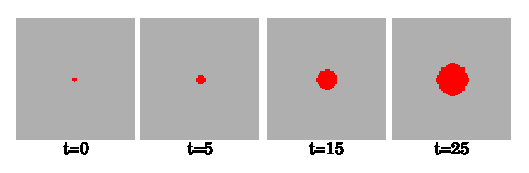
\includegraphics[width=\textwidth]{urban-growt-transitions-1}
      \caption{Růst města bez dalších dodatečných podmínek} 
    \end{subfigure}
    \\
    \begin{subfigure}[t]{\textwidth} \centering
      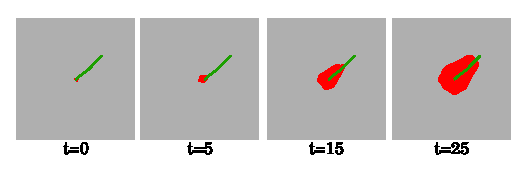
\includegraphics[width=\textwidth]{urban-growt-transitions-2}
      \caption{Růst města podél silnice} 
    \end{subfigure}
    \\
    \begin{subfigure}[t]{\textwidth} \centering
      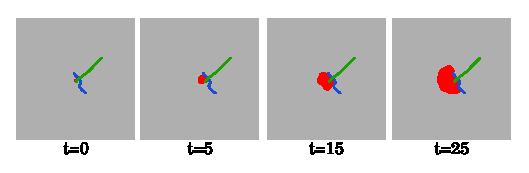
\includegraphics[width=\textwidth]{urban-growt-transitions-3}
      \caption{Růst města bržděn řekou} 
    \end{subfigure}

    \caption[Ukázky chování automatu]{(převzato z \cite{LiuPhi-DevCelAutModUrbGroIncFuzSetApp}, upraveno) Ukázky chování automatu při různých počátečních konfiguracích. Šedě jsou znázorněny prázdné parcely, červeně zástavba, zeleně hlavní silnice a modře řeky.} \label{img-VarTransRuls}
\end{figure}

Na obrázku \ref{img-UrbGroProSample} je k vidění konkrétní ukázka městského růstu. Na obrázku jsou pro porovnání zobrazeny jak vypočtené stavy zástavby, tak i skutečné (upravené satelitní snímky). Na snímcích je patrné, že simulace rozvoje mezi lety 1987 a 1997 dosáhla poměrně přesných výsledků. Stejně tak, v simulaci růstu mezi lety 1997 a 2005 naznačuje jen malý rozvoj. Při simulaci od roku 1987 do roku 2005 už jsou patrné větší odlišnosti (simulace nevyprodukovala tak výrazný růst, jaký doopravdy nastal).

\begin{figure}[]
    \begin{subfigure}[t]{\textwidth} \centering
      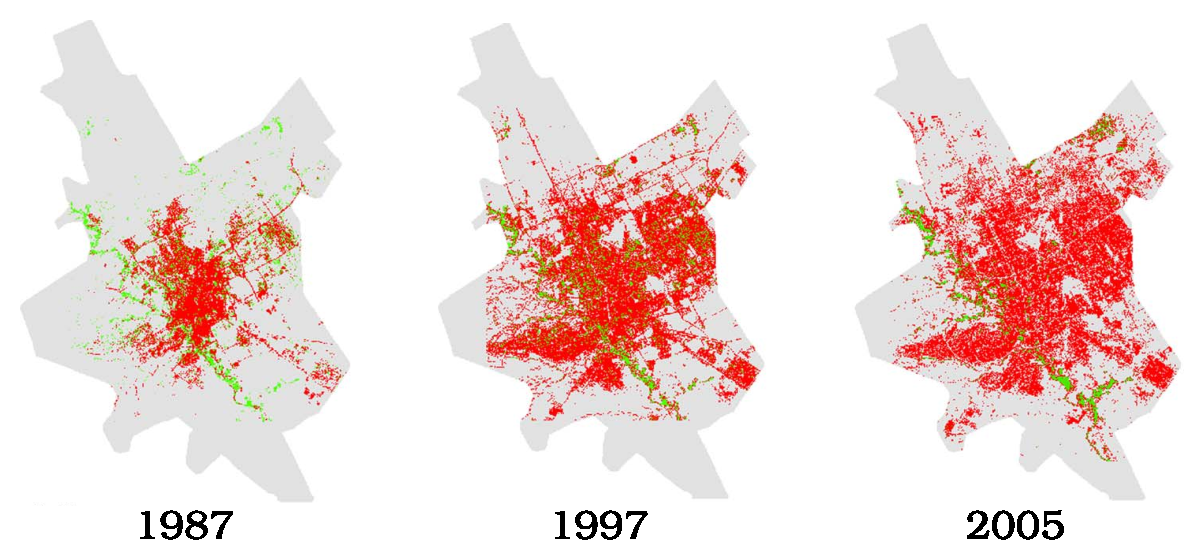
\includegraphics[width=\textwidth]{urban-growt-city-1}
      \caption{Skutečný stav zástavby v uvedeném roce. Červená značí zástavbu, zelená přírodní oblasti (např. vodní plochy) a šedá nezastavěné plochy.} 
    \end{subfigure}
    \\
    \begin{subfigure}[t]{\textwidth} \centering
      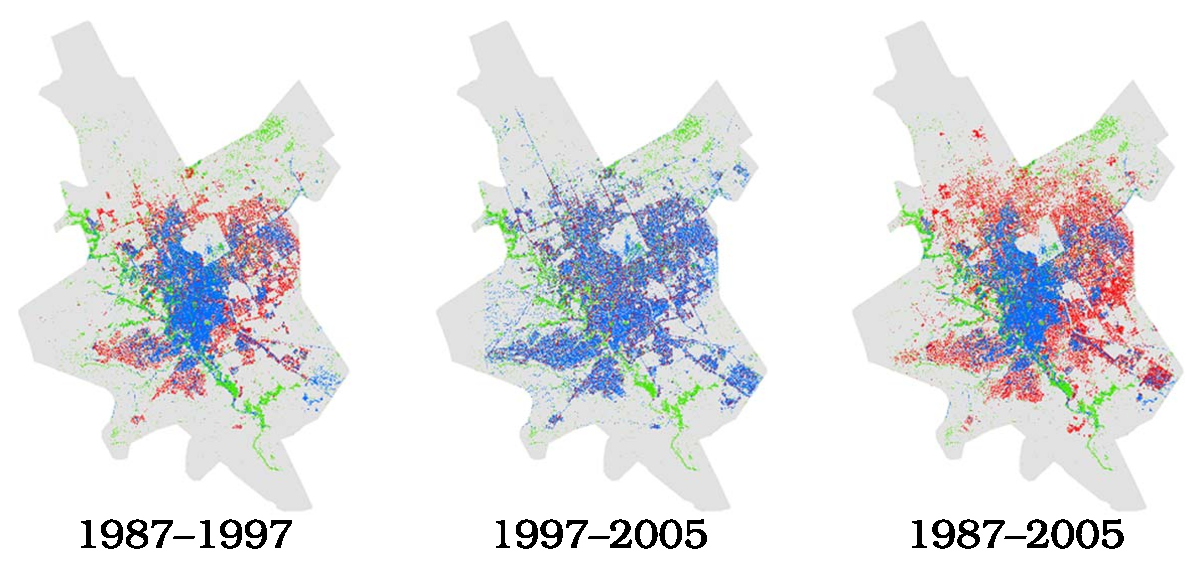
\includegraphics[width=\textwidth]{urban-growt-city-2}
      \caption{Simulovaný stav zástavby. Modrá značí zástavbu na počátku sledovaného období, červená značí (novou) zástavbu na konci sledovaného období, zelená přírodní oblasti (např. vodní plochy) a šedá nezastavěné plochy.} 
    \end{subfigure}

    \caption[Ukázky simulace městského růstu]{(převzato z \cite{Ahm+-CalFuzCelAutModUrbDynSauAr}) Ukázky simulace městského růstu} \label{img-UrbGroProSample}
\end{figure}


%%%%%%%%%%%%%%%%%%%%%%%%%%%%%%%%%%%%%%%%%%%%%%%%%%%%%%%%%%%%%%%%%%%%%%%%%%%%%%%
\subsection{A co na to učící?}
\subsubsection{Něco}
V \cite{TzaRig-StaAnaAdaFuzzConSysUsiPetrNetLeaAut} používají učící se fuzzy automaty v mírně pozměněné formě k řízení výkonu při obloukovém sváření. Abeceda v tomto případě obsahuje dva symboly, \uv{zvýšení výkonu} a \uv{snížení výkonu}. Automat byl sestaven tak, aby správně rozpoznával vhodné posloupnosti zvýšení a snížení výkonu za účelem zvýšení kvality sváru. V téže publikaci demonstrují obdobným způsobem uplatnění pro řízení robota pohybujícího se v neznámém prostředí. Pomocí dvojice symbolů pro zvýšení výkonu motorů a snížení výkonu motorů si kladou za cíl navržení systému pro řízení robota. Tento systém má za cíl řídit přidávání a ubírání výkonu tak, aby se robot, bez ohledu na terén, pohyboval konstantní rychlostí.

\subsubsection{Něco}
V \cite{WeeFu-FormFuzAutAppModLeaSys} je fuzzy automat použit pro návrh řídících systému. Řídící systém je stavový stroj, který je překlápěn mezi diskrétními stavy pomocí událostí. Množina možných událostí tak tvoří abecedu a řídící systém může být reprezentován automatem. Použitím nepřesností je tak možno získat fuzzy automat. \TODO{osamostatnit definici řídícího systému? Např. do ůvodu, kde budu zmiňovat, co všechno se podobá FA?} S pomocí znalosti očekávaného chování systému je pak možné pomocí učícího automatu sestavit adekvátní řídící systém.

\subsubsection{Něco}
V \cite{FuLi-ForLeaAutAutGam} jsou učící automaty použity jako agenti v hře s nulovým součtem, která nemá jasné ekvilibrium. Automaty se postupným hraním tahů učí a vylepšují svoji strategii tak, aby bylo dosaženo ekvilibria.

\subsubsection{Něco}
V \cite{PedGac-LeaFuzzAut} navrhují používat učení fuzzy automatů pro konstrukci logických klopných obvodů. Tj. obvodů, které se na základě vstupů překlápí mezi různými diskrétními stavy. Sami autoři uvádějí, že bylo výhodné pracovat s učícím fuzzy automatem a teprve poté jej \uv{diskretizovat}, tj. konvertovat na kýžený bivalentní.


\subsection{Modelování vytíženosti počítačové sítě}

V \cite{Niz-ModComComNetViaPrAu} modelují pomocí pravděpodobnostního automatu počítačovou síť (zvlášť uzly a kanály, jejich matice pak matematicky spojují do jedné velké matice \uv{matice automatu sítě}). Stavy uzlu jsou délky front v bufferech u jednotlivých kanálů. (U kanálů nevím.) Výsledkem je návrh optimální směrovací tabulky pro celou síť. 

\subsection{Sledování aspektů tvrzení}
V \cite{Cas+-ProAutAspBasSenAna} pomocí pravděpodobnístních automatů analyzují aspektová tvrzení (tj. zda-li je tvrzení míněno pozitivně, negaitvně, neutrálně nebo s rozporem). Stavy automatu jsou všechna slova z celé databáze, vstupní abeceda taktéž. Počáteční stav je první slovo tvrzení, koncový pak poslední. Pravidla jsou, pochopitelně, sestavena učením. Přechody automatu mohou popisovat fráze či použití stejných slov v různém kontextu. Každý stav má pak přiřazenu polaritu, zkomibnováním všech polarit napříč celým tvrtením (napčíř všemi stavy) se pak obdrží celková polarita tvrzení.

\subsection{Generátor strojového člověka}
V \cite{SchYou-ProSimHumMacDia} používají automat jako generátor strojového člověka, konkrétně jako pracovníka banky. Generuje dotazy a, a na základě podnětů od člověka získává informace, co a jak chce (v jejich příkladě, bankovním pracovníku, jestli chce člověk vybrat peníze, nebo provést transakci z účtu na účet). \TODO{Tak ale tohle je spíš práce pro gramatiky, ne?}


\subsection{Metoda lisování dat}
\TODO{zkusit nějaký známý dataset, něco z toho, co jsme dělali v KMI/ZZD}
Autor práce prezentuje novou, jednoduchou, techniku strojového učení. Výhodou této techniky je, že je založena čistě na teorii fuzzy automatů, není třeba žádné další techniky strojového učení.

Vstupem této techniky je (konečná a neprázdná) množina trénovacích dat ve formě jazyka $L$ nad známou abecedou $\Sigma$ a koeficient přesnosti $\sigma$. Výstupem je poté fuzzy automat $A_{L,\sigma}$, který jazyk $L$ přijímá tak, že pro všechna $w \in L$ platí:
$$
  A_{L,\sigma}(w) \geq \sigma
$$
tj. že řetězec $w$ je automatem přijímán alespoň ve stupni $\sigma$. U řetězců, které do jazyka $L$\footnote{Jazyk $L$ může být klidně fuzzy jazyk, následný postup se pak jen patřičně upraví} nepatří (tj. $w' \in \Sigma^* \setminus L$) by posléze měl automat být schopen určit jak moc se jazyku $L$ podobají, tj. určit stupeň $A_{L,\sigma}(w')$.

Postup konstrukce automatu $A_{L,\sigma}$ je násleudjící:
\begin{enumerate}
 \item Máme jazyk $L$, který je konečný. Je tedy zřejmě i regulérní.
 \item K jazyku $L$ sestavíme nedeterministický konečný automat $A_{L}$ rozpoznávající $L$. Takový automat bude v nejhorším případě obsahovat $\sum_{w \in L} |w|$ stavů.
 \item K automatu $A_{L}$ vytvoříme nedeterminstický fuzzy automat $A'_{L}$.
 \item Fuzzy minimalizací automatu $A'_{L}$ se stupněm $\sigma$ získáme hledaný automat $A_{L,\sigma}$.
\end{enumerate}

Klíčovým bodem této techniky je minimalizace automatu. Technika předpokládá, že jazyk trénovacích dat v sobě obsahuje jeden nebo více jednoduchých regulérních jazyků (ať už jako podmnožiny nebo jako podřetězce vybraných řetězců). Části automatu reprezentující tyto \uv{podjazyky} budou minimalizací zmenšeny. Ve výsledku se tak dá očekávat značné zmenšení velikosti automatu.

Navíc, vygenerovaný automat poměrně přehledně popisuje strukturu ve vstupním jazyce. Technika tak může být použita pro odtranění šumu a nepřesností v jazyce $L$.

Technika lisování dat bude naimplementována a experimentálně ověřena. \TODO{naprogramovat, ověrit} Jednou z možností, kde by mohla tato technika být uplatněna, by bylo určování síly přihlašovacícho hesla. Vstupem by byla databáze uživatelských hesel s informací od experta, která hesla jsou silná a která slabá. Ze silných hesel by poté byl sestaven jazyk, na který by bylo aplikováno lisování dat. Výsledkem by byl automat, který rozpoznává silná hesla. Tato aplikace však nebyla naimplementována, vzhledem k tomu, že je z bezpečnostních důvodů nemožné získat databázi uživatelských hesel.

Další z možných aplikací je určování dělitelnosti čísel. Uvažujme abecedu symbolů číslic, tj. $\Sigma = \{ 0, \dots, 9 \}$ a jazyk $L \subseteq S^*$ čísel dělitelných čtyřmi. Při velikosti jazyka $x$ a koeficientu $\sigma = y$ se podařilo automatu dosáhnout $z$ úspěšného rozpoznávání čísel dělitelných $4$ ve stupni vyšším, než $w\%$. \TODO{naprogramovat, ověrit}

Podobnou techniku používají v \cite{Hac+-ProAnaLarFinStaMac}, jen s pravděpodobnostními automaty.


%%%%%%%%%%%%%%%%%%%%%%%%%%%%%%%%%%%%%%%%%%%%%%%%%%%%%%%%%%%%%%%%%%%%%%%%%%%%%%%
%%%%%%%%%%%%%%%%%%%%%%%%%%%%%%%%%%%%%%%%%%%%%%%%%%%%%%%%%%%%%%%%%%%%%%%%%%%%%%%
%%%%%%%%%%%%%%%%%%%%%%%%%%%%%%%%%%%%%%%%%%%%%%%%%%%%%%%%%%%%%%%%%%%%%%%%%%%%%%%
\section{Biologie a medicína}

Biologie a medicína jsou odvětví, které zpravidla disponují velikým množstvím dat, které je třeba zpracovat. Typicky v datech získaných nějakým sledováním najít určité vzory. Fuzzy automaty mohou být v této oblasti nápomocny.

Vzhledem k tomu, že většina těchto aplikací vyžaduje zásah experta na danou problematiku, budou tyto aplikace rozbrány pouze teoreticky.


\subsection{Rozpoznávání řetězců DNA}


Mělo by to jít, něco málo na to mám. \cite{SnaKepAbrHas-AproxStriMatchFuzzAut}



\subsection{Simulace růstu mořských řas}

\cite{CheMyn-ModAlgBloDutCosWat+}. \TODO{odkázat se na urban growt problem}.

\subsection{Rozpoznávání vzorů v lékařských snímcích}
Viz buněčné automaty a jejich jednoduché rozpoznávání vzorů.

A pak ještě toto: \cite{PatPal-FuzGraSynRecSkeMatXra}.

\subsection{Analýza zdravotního stavu pacienta}
V \cite{Jia+-ExHeaSimMetBasIntHumTheMod}, \cite{GupRah-CliMonUsFuzSys}, \cite{CamMerNun-UsFuzAutDiagPrHeaPro} a \cite{SteAdl-CliMonFuzAut} je popisován způsob, jak pomocí fuzzy automatů sledovat zdravotní stav pacienta. 


Technika pracuje s automatem s fuzzy If-Then pravidly. Stavy automatu v tomto případě reprezentují choroby (popř. stavy jedné choroby), přechodová funkce pak přechody mezi nimi. Přechodová pravidla, navržena expertem, pak popisují přechody při různých událostech či akcích (např. medikace). 

Důležitým předpokladem, který automat musí splňovat, je tzv. vlastnost pozdržení vrcholu\TODO{nadefinovat někde v úvodech?}. Tato vlastnost říká, že výpočet automatu pro libovolný vstup nikdy nezkončí v prázdném fuzzy stavu, tj. výpočet se vždy bude muset nacházet v nenulovém stupni v alespoň některém stavu.

\TODO{Příklad?}

Fuzzy stav automatu v \cite{GupRah-CliMonUsFuzSys} nazývají \uv{fuzzy chorobný syndrom}. Fuzzy chorobný syndrom je vlastně popis zdravotního stavu pacienta v určitý okamžik. 

Tato technika tak může sloužit ke porovnávání simulovaného a skutečného stavu (např. po medikaci, zákroku) pacienta a případně včas reagovat na odchylku. Výhodou této techniky je, že značně zjednodušuje sledování více diagnóz současně.

V \cite{GupRah-CliMonUsFuzSys} tuto techniku používají pro sledování systolického krevního tlaku a množství krevního cukru. V \cite{Jia+-ExHeaSimMetBasIntHumTheMod} používají podobnou techniku pro sledování těla při sportu (konkrétně tělní teplotu, dehydrataci a srdeční tep).

V \cite{CamMerNun-UsFuzAutDiagPrHeaPro} se fuzzy automaty používají pro diagnózu srdečních chorob. Po spuštění automat na základě pohlaví a věkové skupiny přejde do odpovídajícího podautomatu. Ten si poté sám žádá měření různých parametrů (aktuální tepová frekvence, aktuální variabilita srdeční frekvence) v závislosti na tom, kdy je který pro proces diagnózy aktuálně významný. V případě stanovení rizika je riziko ohlášeno a automat se vrací do počátečního stavu a proces se spouští znovu (aby diagnózu ověřil). 


% \subsection{Diagnóza a predikce chorob srdce}
% V \cite{CamMerNun-UsFuzAutDiagPrHeaPro} je prezentována technika pro diagnózu a predikci chorob či problémů srdce. Využívají k tomu fuzzy automat s fuzzy If-Then pravidly a výstupem. 
% 
% Přechodová funkce je realizována pravidly sledující určité vlastnosti pacienta (pohlaví, věk, aktuální tepová frekvence, aktuální variabilita srdeční frekvence). První dvojicí přechodů je rozlišení pohlaví a věkové kategorie (fuzzy množiny) pacienta. Na základě těchto vlastností výpočet pokračuje v patřičném podautomatu. Jednotlivé podautomaty tak mají detekci problémů přizpůsobenu přímo věku a pohlaví pacienta.
% 
% Vzhledem k tomu, že tepová frekvence i variabilita srdeční frekvence se u pacienta mohou měnit v závislosti na čase, podautomaty mohou obsahovat smyčky, díky kterým může být měření těchto vlastností prováděno opakovaně (po určitém počtu \uv{negativních} měřeních se však výpočet automaticky ukončuje). 
% 
% Podautomaty (především stupňě pravdivosti a meze hodnot u přechodů) jsou navrženy expertem. Pokud se výpočet podautomatu dostane do stavu reprezentující srdeční problém, je proveden přechod s výstupem (varovné hlášení) zpět do počátečního stavu podautomatu a celý proces je spuštěn znovu. Počet vygenerovaných varovných hlášení je poté směrodatný spolu se stupněm pravdivosti (tzv. úroveň spolehlivosti), v jakém výpočet automatu zkončil\footnote{Nízká hodnota značí, že výpočet automatu neproběhl zcela dle očekávání a napočítaný počet varovných hlášení tak nemusí být zcela směrodatný}. Autoři navíc doporučují počítat úroveň spolehlivosti dvakrát, pokaždé s jinou $t$-normou (v jejich případě Gödelova t-norma a Hamacherův produkt).
% 
% \TODO{Příklad?}
% 
% Autoři techniku ověřili experimentálně na vybraných vzorcích z databáze případových studií. V článku jsou odprezentovány výsledky pro 31 pacientů analyzované podautomaty pro muže a ženy ve věku 60 -- 69 let (tj. vzhledem k odstuňovanosti $\pm 13$ let). Autoři výsledky nijak statisticky neanalyzují, zaměřují se na popis konkrétních pacientů a důvody, proč u nich došlo k odchylce (zmiňují např. sportovní aktivity či vrozené předpoklady). Autoři uvádějí, že možným vylepšením by mohlo být provázání se strojovým učením.
% 
% \TODO{uvést, že v sledovat všechny možné hrozící diagnózy je pro (1) lékaře nemožné, ale mít automat pro každou diagnózu zvlášť ... }

\TODO{nadefinovat u různých typů automatů Fuzzy automat (klasický nedeterminstický) s If-Then pravidly} \TODO{On je vlastně i rozdíl mezi fuzzy automatem s If-Then pravidly a bivaletním automatem s fuzzy If-Then pravidly}

\TODO{terminologie u proměnných (resp. indexů proměnných), česky (triangel, age, distance) vs. česky?}


\subsection{Detekce zhoubných nádorů}
V \cite{Est+-CytImAnaGenFuFiStMa} popř. \cite{Est+-CytImAnaGenFuFiStMa} využívají učící se fuzzy automat pro rozpoznávání zhoubných (maligních) nádorových buněk. Vstupem této techniky je mikroskopický snímek z buněk z prsní tkáně, výstupem pak nalezené maligní buňky. Využívají faktu, že nezhoubné buňky mají na snímcích obvykle symetričtější tvary a méně \uv{skvrn}.

Proces rozpoznávání probíhá následujícím způsobem:
\begin{itemize}
 \item Snímek je převeden do odstínů šedi.
 \item Jednotlivé buňky na snímku jsou izolovány do samostatných obrazů. Následně jsou zpracovávány všechny obrazy postupně.
 \item Na obraze jsou rozpoznány plochy stejné nebo podobné barvy.
 \item Z ploch je na základě relace \uv{plocha $X$ obsahuje plochu $Y$} zkonstruován strom ploch.
 \item Strom je následně zakódován do řetězce a rozpoznán fuzzy automatem.
\end{itemize}

Stromy jsou do řetězců kódovány jako posloupnost čísel, kde každé číslo odpovídá počtu potomků jednotlivých uzlů stromu. Automat byl sestaven učením z veřejné databáze snímků. Autoři poukazují, že tato technika je na rozpoznávání účinější, než vybranné z dalších tehcnik.

\TODO{ukázka?} 

\subsection{Analýza kardiogramu}
Např. \cite{PedGac-LeaFuzzAut}, popř. i \cite{RigTza-FuzAutFauDia}. Ale je to obecně zpracování signálu, popsat někde jinde?

\subsection{Řízení protézy}
V \cite{Alv-HumGaiModUsGenFuzFinStaMac} (popř. i \cite{AlvTri-ComModQuaPerSig} \TODO{to by šlo ale obecně použít pro zpracování signálu, ne?})
používají fuzzy automaty pro modelování fungovaní protézy dolní končetiny. Pomocí akcelerometrů sledují pohyb patřičné náhrady a pomocí známých vzorů spouštějí automat, který určuje, v jaké fázi pohybu protéza je.

\subsection{Modelování buněčných sítí}

V \cite{MilAtl-ProAuModEpiCelNet} používají pravděpodobnostní automaty na epigenetiku. Princip je podobný, jak u buněčných automatů, jen množina \uv{buněk} není pevně daná. Jinými slovy neuvažuje se mřížka živých a neživých buněk, ale množina jen těch živých, která se postupně rozrůstá (popř. odumírá). Každá buňka se nachází v některém stavu z množiny stavů (jako je např. \uv{buňka se zrodila}, \uv{buňka je přípravena k dělení}, \uv{buňka je rodičovskou buňkou jiné buňky}). Přechodová pravidla poté v periodických časových kvantech provádějí přechody mezi těmito stavy. Například je-li buňka \uv{připravena k dělení}, pak v dalším kroku provede dělení, tj. vytvoří novou buňku ve stavu \uv{buňka se zrodila} a buňka samotná přechází do stavu \uv{buňka je rodičovskou buňkou jiné buňky}. Díky využití pravděpdobnostních automatů se takovéto modely mohou znače více přiblížit reálným buněčným sítím.

\subsection{Modelování šíření infekční nemoci}
V \cite{BocChe-CriBePrAuNetModSprInfDis+} používají systém podobný pravděpodobnostnímu buněčnému automatu pro modelování šíření infekčních nemocí. Každá buňka je buďto prázdná nebo se v ní nachází osoba. Osoba může být ve stavu \uv{nenakažena} nebo \uv{nakažena}. Nachází-li se v okolí \uv{nenakažené} osoby $q$ alespoň jedna nakažená osoba, pak s pravděpodobností $p$ přejde při dalším časovém kroku do stavu \uv{nakažena}, jinak zůstává ve stavu \uv{nenakažena}. 

Autoři navíc do modelu zanášejí pohyb jedinců, tj. že s určitou pravděpodobností se může osoba na buňce $c$ přesunout na některou sousední buňku $c'$ je-li neobsazena. Změnou parametrů systému (jednotlivých pravděpodobností) tak lze nasimulovat vymícení choroby nebo naopak vznik epidemie.

%%%%%%%%%%%%%%%%%%%%%%%%%%%%%%%%%%%%%%%%%%%%%%%%%%%%%%%%%%%%%%%%%%%%%%%%%%%%%%%
%%%%%%%%%%%%%%%%%%%%%%%%%%%%%%%%%%%%%%%%%%%%%%%%%%%%%%%%%%%%%%%%%%%%%%%%%%%%%%%
%%%%%%%%%%%%%%%%%%%%%%%%%%%%%%%%%%%%%%%%%%%%%%%%%%%%%%%%%%%%%%%%%%%%%%%%%%%%%%%
\section{Zpracování obrazu}

\subsection{Konvoluce}
Zpracování obrazu je v dnešní době velmi populární informatická disciplína. Jak bude ukázáno, nasazení buněčných fuzzy automatů zde nachází značné uplatnění.

Uvažujme obraz jako mřížku $m \times m$ pixelů s odstíny šedi jako hodnotami od $0$ do $1$. Hodnota $0$ značí černou, hodnota $1$ bílou. Jinými slovy, barva (resp. stupeň šedi) pixelu odpovídá stupni pravdivosti tvrzení \uv{pixel má bílou barvu}. Tato skutečnost nám umožňuje pracovat s obrazem pomocí fuzzy logiky.

Každý obraz tak můžeme považovat za konfiguraci buněčného fuzzy automatu s množinou stavů $Q = [0,1]$. Návrhem vhodné přechodové funkce tak můžeme vytvořit automat, který provádí určitou operaci pro úpravu obrazu. Typickou operací je tzv. obrazový filtr, který obrazu $m \times m$ přiřazuje obraz $m \times m$.

Speciálním případem takového automatu je automat realizující konvoluční metodu \cite{Rus-ImaProHan}. Konvoluce je v základu obrazový filtr, který přiřazuje (novou) hodnotu pixelu na základě váženého součtu (stávající) hodnoty pixelu a hodnot pixelů sousedních. Váhy bývají reprezentovány tzv. konvoluční maticí. Například matice
$$
  B = \begin{pmatrix}
       1 & 2 & 1 \\
       2 & 4 & 2 \\
       1 & 2 & 1 
      \end{pmatrix}
$$
je konvoluční maticí jednoduchého rozostření. Aplikuje se následujícím způsobem:
$$
  c'_{i,j} = \frac{1}{S} \sum_{k,l \in \{-1, 0, +1\}} B_{k+1, l+1} c_{i+k, j+l}
$$
kde $S$ je součet hodnot v matici $B$, tj. $16$.

Další ukázkou grafického filtru pracujícího s využitím buněčného fuzzy automatu je například filtr pro zvýraznění tvarů. Je daný následujícím předpisem
$$
  c'_{i,j} = \max(0, \min(1, 
    \begin{dcases}
      \epsilon (c_{i,j} + 1) - 1	& \text{pokud $c_{i,j} > neighs_{i,j}$} \\
      \epsilon c_{i,j}			& \text{pokud $c_{i,j} < neighs_{i,j}$} \\
      c_{i,j}	& \text{pokud $c_{i,j} = neighs_{i,j}$} 
    \end{dcases}
    ))
$$
kde $\epsilon > 1$ je parametr udávají agresivitu zvýrazňování a $neighs_{i,j}$ je součet hodnot okolních buňek (viz příklad \ref{ex:GameOfLife}).

Ukázky aplikací obou filtrů jsou k nalezení na obrázku \ref{img:Filters}. V následujících podkapitolách budou prezentovány některé další (pokročilejší) techniky zpracování obrazu využívající buněčné fuzzy automaty.

\begin{figure}[]
 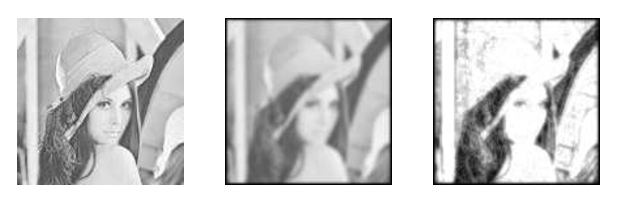
\includegraphics[width=\textwidth]{filters}
 
 \caption{Ukázky jednoduchých filtrů. Vlevo původní obrázek, uprostřed obrázek po $5$ generacích jednoduchého rozostřovacího filtru a v pravo obrázek po $8$ generacích filtru pro zvýraznění tvarů ($\epsilon = 1,1$).} \label{img:Filters}
\end{figure}

\subsection{Hledání hran}
Hledání hran je jednou ze základních technik zpracování obrazu. Hledání hran je často klíčové pro rozpoznávání vzorů v obrazech. V dnešní době existuje značné množství technik pro rozpoznávání hran \cite{MaiAgg-StuComVarImDetEdTec}. V \cite{MarMeySol-HybMetGasDifModFuzCelAutImSha} je popsán poměrně elegantní způsob, jak hledání hran vyřešit pomocí buněčných fuzzy automatů.

Označme osmici směrů dle obrázku \ref{img:Directions:8Directions}. Množinu těchto směrů nazvěme $dim$. Dále označme $c_X$ (kde $X \in dim$) jako sousední buňku buňky $c$ ve směru $X$.

\begin{figure}
   \begin{subfigure}[t]{0.4\textwidth}
      \includegraphics[width=\textwidth]{miscs0}
      \caption{8 směrů}  \label{img:Directions:8Directions}
    \end{subfigure}%
%
    \begin{subfigure}[t]{0.4\textwidth}
      \includegraphics[width=\textwidth]{miscs1}
      \caption{Ukázka hrany procházející buňkou. Ve směru $U$ (červené šipky) prochází hrana, ve směru $R$ (zelené šipky) neprochází.}  \label{img:Directions:Edges}
    \end{subfigure}
\end{figure}

Autoři vycházejí z následující úvahy: Prochází-li buňkou $c$ hrana ve směru $X \in dim$, pak má buňka $c_X$ výrazně jinou barvu, než buňka $c$ (viz obrázek \ref{img:Directions:Edges}). Prochází-li buňkou $c$ hrana v alespoň jednom směru $X \in dim$, pak můžeme říci, že buňka obsahuje hranu.

Nadefinujme fuzzy relaci \uv{buňky $c$ a $c'$ mají zcela rozdílnou barvu} předpisem:
$$
  \Delta(c, c') = 1 - | c - c' |
$$

Označme $\Delta'$ jako doplňek k $\Delta$, tedy \uv{buňky $c$ a $c'$ mají zcela shodnou barvu}. Pak můžeme stanovit fuzzy množiny $\epsilon_X$ (pro všechny $X \in dim$) ve smyslu \uv{buňkou $c$ prochází hrana ve směru $X$}. Pro $X = U$ by pravidla vypadala následovně:
\begin{itemize}
 \item Pokud $\Delta'(c_{L}, c_{UL})$, $\Delta'(c, c_{U})$ a $\Delta'(c_{R}, c_{UR})$ pak $\epsilon_U(c) = 0$
 \item Pokud $\Delta (c_{L}, c_{UL})$, $\Delta (c, c_{U})$ a $\Delta (c_{R}, c_{UR})$ pak $\epsilon_U(c) = 1$
\end{itemize}

Obdobným způsobem by se dodefinovaly zbývající fuzzy množiny $\epsilon_X$. Následně lze nadefinovat fuzzy množinu $\epsilon$ ve smyslu \uv{buňkou $c$ prochází hrana} pomocí pravidel:
\begin{itemize}
 \item Pokud $c = \epsilon_{U}$ pak $\epsilon = 1$
 \item $\dots$
 \item Pokud $c = \epsilon_{UR}$ pak $\epsilon = 1$
 \item Jinak $\epsilon = 0$
\end{itemize}

Pomocí těchto pravidel tak lze sestavit buněčný fuzzy automat s fuzzy logikou, který rozpoznává hrany. 

Dle \cite{MarMeySol-HybMetGasDifModFuzCelAutImSha} může být hodnota stupně \uv{buňkou $c$ prochází hrana} použita jako parametr $\alpha$ tzv. Gas Diffusion Modelu, jednu z technik zaostřování obrazu.

%%%%%%%%%%%%%%%%%%%%%%%%%%%%%%%%%%%%%%%%%%%%%%%%%%%%%%%%%%%%%%%%%%%%%%%%%%%%%%%
\subsection{Ostraňování šumu}
Odstraňování šumu je další častý problém, který je třeba při zpracování obrazů řešit. Pro studium technik odstraňování šumu se používá zašumnění tzv. impulzním šumem popř. šumem \uv{sůl a pepř}. Zašumnění impulzním šumem nahradí stanovený počet pixelů náhodnými barvami. Šumění \uv{sůl a pepř} pak narazuje pixely buď bílou ($1$) nebo černou ($0$) barvou.

V \cite{SadRetKam-EfMetImpNoiRedImFuzCelAut} je prezentována jednoduchá avšak efektivní technika, která kombinuje klasický bivalentní buněčný automat s buněčnýcm fuzzy automatem. 

V první fázi je klasickým buněčným automatem šum detekován. Buňka obsahuje šum, pokud rozdíl její barvy od průměrné barvy jejich sousedů překračuje stanovenou mez. Tato mez může být stanovena statisticky, například na základě směrodatné odchylky barev pixelů celého obrazu. V druhé fázi je aplikován buněčný fuzzy automat, který buňky obsahující šum nahradí hodnotami spočtenými z jejich okolí. 

Jak autoři poukazují, tato technika je na odstraňování šumu velmi efektivní. Ukázky výsledků jsou na obrázku \ref{img:Noises}. 

\begin{figure}
   \begin{subfigure}[t]{0.3\textwidth}
      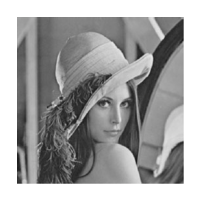
\includegraphics[width=\textwidth]{noises1}
      \caption{Vstupní obraz}  
    \end{subfigure}%
%
    \begin{subfigure}[t]{0.3\textwidth}
      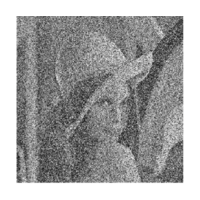
\includegraphics[width=\textwidth]{noises2}
      \caption{Zašumněný obraz}
    \end{subfigure}%
%
    \begin{subfigure}[t]{0.3\textwidth}
      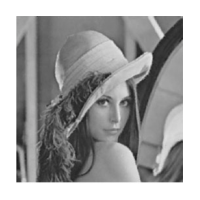
\includegraphics[width=\textwidth]{noises3}
      \caption{Obraz s odstraněným šumem}
    \end{subfigure}
    
    \caption{(převzato z \cite{SadRetKam-EfMetImpNoiRedImFuzCelAut}) Ukázka odstraňování šumu} \label{img:Noises}
\end{figure}

Velmi podobný způsob ostranění šumu je popsán v \cite{SahUguSah-SalPepNoiFilFuzCelAut}. Zde však operace detekce šumu a jeho odstranění provádějí v jednom kroku.

%%%%%%%%%%%%%%%%%%%%%%%%%%%%%%%%%%%%%%%%%%%%%%%%%%%%%%%%%%%%%%%%%%%%%%%%%%%%%%%
\subsection{Rozpoznávání jednoduchých vzorů}

Ropoznávání vzorů je další z častých způsobů práce s obrazy. Obecně je problém definován (obdobně, jako rozpoznávání textových vzorů v kapitole \TODO{ref na kapitolu}) jako problém určení, zda-li obraz obsahuje předem stanovený vzor či ne. Obvykle nás také zajímá, kde přesně se vzor v obraze vyskytuje.

Rozpoznávání vzorů v obrazech je však značně komplikované i pro buněčné fuzzy automaty. V \cite{MajCha-FuzCelAutModPatClas} je popsán způsob, který popisuje rozpoznávání vzorů v obrazu velikosti $1 \times m$ pomocí (jednodimenzionálního) buněčného automatu. Pomocí fuzzy množin reprezentující různé stupně šedi jsou sestavena pravidla, která popisují jak vzorový obraz, tak obrazy jemu podobné. Množina přechodových pravidel tak vyjmenovává téměř všechny možné kombinace hodnot fuzzy množin pro všechny buňky v okolí. Velikost přechodové funkce je tak exponenciální vzhledem k velikosti okolí buňky. Vzhledem k tomu, že okolí buňky je vlastně předpisem pro vzor, je tato technika nepoužitelná pro vzory větší než jednotky pixelů.

Zcela jiný přístup pužívají v \cite{WanJiaZhoDu-ImProcBasFuzCelAuMod}. Vzor nepovažují jako konkrétní kombinaci odstínů barev, ale jako část obrazu splňující určité vlastnosti.

Autoři metodu doporučují na vyhledávání vzorů v lékařských snímcích (např. ultrazvuk, Röntgen). Techniku demonstrují na ultrazvukových snímcích vaječníků. Poukazují na to, že folikula\footnote{Folikula je dutinka ve vaječníku, v níž probíhá zrání vajíčka. \TODO{ocitovat: http://lekarske.slovniky.cz/pojem/folikul}} je na snímku tvořena jednolitou svrnou stejné barvy, obklopena ostatní tkání (barevné přechody). Ukázka několika snímků je k dispozici na obrázku \ref{img:Follicles:Screens}. Obecně tak lze hovořit o \uv{popředí} (folikula) vystupující z \uv{pozadí}.

K nalezení popředí používají dvojici buněčných fuzzy automatů. První automat určuje hodnotu \uv{buňka je kandidát na buňku folikuly}. Druhý automat pak buňky, které nebyly označeny jako kandidáti, ostraňuje (nastavuje na $0$).

Přechodová funkce první automatu je poměrně složitá, pracuje s 5 stupni šedi a třemi stupni kandidatury, takže zde nebude rozebírána. Druhý automat pak funguje elementárně. Buňky, jež nejsou označeny jako dostatečné kandidáty na folikuly, jsou odstraněny, ostatní ponechány.

Na obrázku \ref{img:Follicles} jsou k nahlédnutí ukázky rozpoznaných folikul pomocí této techniky.

\begin{figure}
  \begin{subfigure}[t]{\textwidth} \centering
    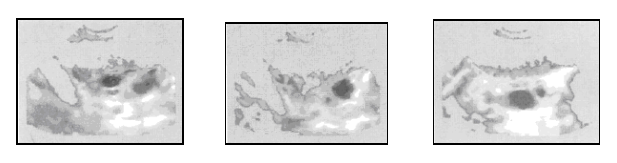
\includegraphics[width=\textwidth]{follicles-1}
    \caption{Ultrazvukové snímky vaječníků} \label{img:Follicles:Screens}
  \end{subfigure}
  \\
  \begin{subfigure}[t]{\textwidth} \centering
    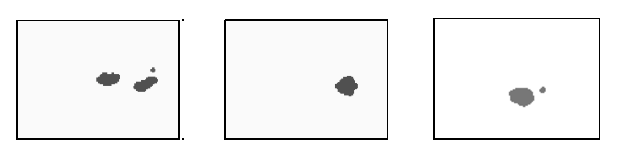
\includegraphics[width=\textwidth]{follicles-2}
    \caption{Rozpoznané folikuly}
  \end{subfigure}
 
  \caption{(převzato z \cite{WanJiaZhoDu-ImProcBasFuzCelAuMod}, upraveno) Ukázky rozpoznávání folikul} \label{img:Follicles}
\end{figure}

%%%%%%%%%%%%%%%%%%%%%%%%%%%%%%%%%%%%%%%%%%%%%%%%%%%%%%%%%%%%%%%%%%%%%%%%%%%%%%%
\subsection{Složené geometrické útvary}

V \cite{Lee-FuzTreAutSynPatRec} byl popsán způsob, jak pomocí fuzzy tree automatů rozpoznávat složené geometrické útvary. Složený geometrický útvar je chápán jako strom, jehož listové uzly reprezentují \uv{primitivní geometrické objekty} (čtverec, kruh, trojúhelník, aj.). Jeho vnitřní uzly pak popisují vzájemný vztah či vlastnost (např. vzájemnou polohu) jednotlivých podobjektů.


\begin{example}
  Na obrázku \ref{img:Geoms} je vyobrazen složený geometrický útvar vyobrazující \uv{budovu kostela} a jemu odpovídající strom.
\end{example}

\begin{figure}[htp]
 \centering
 
 \begin{subfigure}{0.4\textwidth}
  \includegraphics{trees11}
 \end{subfigure}
 %
 \begin{subfigure}{0.4\textwidth}
  \includegraphics{trees12}
 \end{subfigure}
 
 \caption{Příklad složeného geometrického tvaru a jeho stromu} \label{img:Geoms}
\end{figure}

V příkladu, který autoři uvádějí, konstruují strom pro náčrt jednoduchého domu a následně kostela. Dům je tvořen čtvercem (\uv{budova}) a \uv{nad ním} se nachází rovnoramenný trojúhelník (\uv{střecha}). Kostel pak lze vyjádřit jako \uv{dům, nad kterým se nachází kříž}.

Pro rozpozánávání takovýchto stromů fuzzy tree automatem je nutné tyto pojmy nejdříve formalizovat. Jakmile budeme mít pevně stanoveny jednotlivé pojmy, budeme moci provést jejich fuzzyfikaci a následně sestavit fuzzy tree automat, který stromy rozpoznává.

Uvažujme primitivní geometrický útvar $g$. Konkrétní podoba útvaru $g$ bude dána jeho typem. Například mnohoúhelníky budeme reprezentovat jako posloupnosti jejich vrcholů, kružncie bude reprezentována jako střed a poloměr. Připomeňme si nejdříve matematické definice některých základních primitivních geometrických tvarů. \TODO{je to nutné zdrojovat?}

\begin{notation*}
 Pro mnohoúhelník $g$ označme $\alpha_X$ jako velikost úhlu při vrcholu $X \in g$.
\end{notation*}

\begin{definition}[Obdélník]
 Mějme čtyřúhelník $g = A B C D$. Pak tento čtyřúhelník je obdélník, pokud platí
 $$
  \alpha_A = \alpha_B = \alpha_C = \alpha_D ( = 90° )
 $$
\end{definition}

\begin{definition}[Čtverec]
 Mějme obdélník $g = A B C D$. Pak tento obdélník je čtverec, pokud
 $$
  |A B| = |B C| = |C D| = |D A|
 $$
\end{definition}

\begin{definition}[Rovnoramenný trojúhelník]
  Mějme trojúhelník $g = A B C$. Pak tento trojůhelník je rovnoramenný, pokud
  $$
    \alpha_A = \alpha_B
  $$
  Stranu $AB$ nazývejme základna, strany $AC$ a $BC$ ramena.
\end{definition}

Obdobným způsobem bychom ve výčtu mohli pokračovat. Pro užití fuzzy tree automatů však bude vhodné nehovořit o \uv{útvar $g$ je/není obdélník}, ale \uv{útvar $g$ je obdélníkem ve stupni $c$}.

Označme $\varepsilon: \mathbb{R}_0^+ \times \mathbb{R}_0^+ \rightarrow [0,1]$ jako fuzzy ekvivalenci reálných čísel danou předpisem:
$$
  \varepsilon(x, y) =
    \begin{dcases}
     \frac{x}{y}	& \text{pokud $x \leq y$}	\\
     \frac{y}{x}	& \text{pokud $x > y$}
    \end{dcases}
$$
s tím, že $\frac{0}{0} = 1$. Zřejmě platí $\epsilon(x, x) = 1$ pro všechna $x \in \mathbb{R}_0^+$.

S využitím fuzzy ekvivalence $\varepsilon$ tka můžeme předchozí tři definice \uv{fuzzyfikovat}:

\begin{definition}[\uv{Fuzzy} obdélník]
 Mějme čtyřúhelník $g = A B C D$. Pak tento čtyřúhelník je obdélníkem ve stupni $\gamma_r(g)$, kde
 $$
  \gamma_r(g) = \varepsilon(\alpha_A, \alpha_B) 
  \wedge \varepsilon(\alpha_B, \alpha_C)
  \wedge \varepsilon(\alpha_C, \alpha_D)
  \wedge \varepsilon(\alpha_D, \alpha_A)
 $$
\end{definition}

\begin{definition}[\uv{Fuzzy} čtverec]
 Mějme geometrický útvar $g = A B C D$, který je obdélníkem ve stupni $\gamma_r(g)$. Pak tento obdélník je čtvercem ve stupni $\gamma_s(g)$, kde
 $$
 \gamma_s(g) = \gamma_r(g)
  \wedge \varepsilon(|A B|, |B C|) 
  \wedge \varepsilon(|B C|, |C D|)
  \wedge \varepsilon(|C D|, |D A|)
  \wedge \varepsilon(|D A|, |A B|)
 $$
\end{definition}

\begin{definition}[\uv{Fuzzy} rovnoramenný trojúhelník]
  Mějme trojúhelník $g = A B C$. Pak tento trojůhelník je rovnoramenný ve stupni $\gamma_i(g)$, kde
  $$
    \gamma_i(g) = \varepsilon(\alpha_A, \alpha_B)
  $$
\end{definition}

Máme tedy fuzzifikovány vlastnosti primitivních geometrických útvarů. Nyní je třeba navrhnout fuzzyfikace jejich vzájemných vztahů. Pro vztah \uv{být nad} máme například:

\begin{definition}[Vztah \uv{být nad}\footnote{Zde si dovolujeme značné zjednodušení. Vztah \uv{být nad} by měl být popsán například s využitím porovnávání y-ových souřadnic bodů. }]
 Mějme obdélník $r = A B C D$ a trojúhelník $q_t = E F G$. Pak \uv{trojúhleník $r$ je nad obdélníkem $q_t$ (a horní hrana $q_r$ splývá se základnou $t$)} právě tehdy, když:
 $$
  top(r) = base(t)
 $$
 kde $top(r) \in \{ AB, BC, CD, DA \}$ je \uv{horní strana} obdélníku $r$ a $base(t) \in \{ EF, FG, GA \}$ je základna trojúhelníku $t$.
 
 Mějme geometrický útvar $r' = A B C D$, který je obdélníkem ve stupni $\gamma_r(r')$ a trojúhelník $q'_t = E F G$. Pak \uv{trojúhleník $r'$ je nad obdélníkem $q'_t$ (a horní hrana $q'_r$ splývá se základnou $t'$)} ve stupni $\gamma_T(r', t')$, kde
 $$
  \gamma_T(r', t') = \gamma_r(r') \wedge \varepsilon(top(r'), base(t'))
 $$
 a kde $\varepsilon(XY, ZW) = \varepsilon(X, Z) \wedge \varepsilon(Y, W)$ je fuzzy ekvivalence úseček a $\varepsilon(X, Y) = \bigwedge_{i} \varepsilon(X_i, Y_i)$ je fuzzy ekvivalence vrcholů.
\end{definition}

Máme tedy formálně popsány a fuzzifikovány vlastnosti primitivních gemetrických tvarů a (alespoň jednu) vlastnost popisující složený geometrický tvar. Položme $T = \{ r, s, t, i \}$ jako terminály symbolizující obdélník, čtverec, (obecný) trojúhelník a rovnoramenný trojúhelník. Dále stanovme $N = \{ T \}$. Pak pseudoterm $p(t_H) = T(i, s)$ nad $(N, T)$ symbolizuje dům popsaný výše.

Označme $A_H = (Q, N, T, \mu, F)$ jako fuzzy tree automat rozpoznávající strom $t_H$. Označme $A'_H = (Q, N, T, \mu', F)$, kde $\mu'$ vznikla z $\mu$ nahrazením všech $1$ (pro všechna $X \in (N \cup T)$) výrazem $\gamma_X$.

\begin{example}
 Uvažujme složený geometrický útvar $C$ z obrázku \ref{img:Geoms}. Pak automat $A'$ bude nějak vypadat. \TODO{domyslet to nějak!}.
\end{example}

Takto vytvořený automat dokáže rozpoznávat geometrické tvary \uv{podobné} (ve smyslu relací $\gamma$) vzorovému. Nevýhodou tohoto řešení je, že je pevně svázán s aritou (a pořadím potomků) uzlú vzorového stromu. Navíc, stupeň pravdivosti popisující vztah v uzlu $U$ stromu je schopen kalkulovat pouze se svými potomky (a nikoliv například svými sousedy či předky). Obě tyto výhody se však smývají, pokud se bude pozorovaný strom od vzoru lišit jen málo.

I přes tyto nevýhody však lze fuzzy tree automaty použít na podobnostní rozpoznávání složených geometrických tvarů.

\TODO{To samé dělá i v \cite{Lee-AppFuzLanPatRec}, akorát to dělá přes jazyky a gramatiky, ne přes automaty. Ale takových případů jsem měl víc, zmínit je v sekci problémy v metodice!}



%%%%%%%%%%%%%%%%%%%%%%%%%%%%%%%%%%%%%%%%%%%%%%%%%%%%%%%%%%%%%%%%%%%%%%%%%%%%%%%
\subsection{Detekce požárů}
V \cite{HamKoNam-FirFlaDetBasFuzFinAut} a \cite{KoHamNam-ModForFuFiAuDetIrrFirFla} používají fuzzy automaty pro pattern matching ve videosekvenci, konkrétně pro detekci požárů.

V první fázi se snímek rozdělí na několik regionů a na základě barvy (teplé světlé barvy) se určí, zda-li jednotlivé regiony mohou být plamenem (tzv. kandidáti). Pro každého kandidáta je pak sestaven fuzzy automat o čtyřech stavech $q_{VL}, q_{L}, q_{H}, q_{VH}$. Pokud se automat regionu nachází ve stavu $q_VL$, pak platí, že \uv{region je velmi málo pravděpodobné, že je tvořen plamenem}. Obdobně pro $q_{L}$ (\uv{málo pravděpodobné}), $q_{H}$ (\uv{hodně pravděpodobné}) a $q_{VH}$ (\uv{velmi pravděpodobné}). Abecedou událostí jsou pak kombinace dalších atributů (svit, pohyb v určitém směru, vlnění) spočtených z předchozích snímků. Přechodové pravidlo pak může být např. \uv{pokud jsi ve stavu $q_{H}$ a došlo k velkému posunu směrem nahoru a malému snížení svitu, pak přejdi do stavu $q_{VH}$}. Přechodovou funkci pak navrhli statistickým pozorováním známých videosekvencí s požáry\footnote{Dá se říci, že automat vznikl pomocí učení s učitelem}.

Autoři tuto techniku experimentálně ověřili a ukázalo se, že požár detekuje správně ve vyšším množství případů, než některé vybrané další metody. Stejně tak, oproti jiným metodám, technika mnohem méně rozpoznávala požár tam, kde nebyl.
\TODO{vložit obrázek s výsledkem?}


%%%%%%%%%%%%%%%%%%%%%%%%%%%%%%%%%%%%%%%%%%%%%%%%%%%%%%%%%%%%%%%%%%%%%%%%%%%%%%%
\subsection{A co na tu učící?}
\subsubsection{Něco}
V \cite{AstGariGonVillFar-ApprStrMatUsiDefFuzzAutLearExpr} a \cite{WeeFu-FormFuzAutAppModLeaSys} používají učící automat na vylepšení rozpoznávání textu v obrazu. Jako trénovací data jsou použity známé (již dříve rozpoznané) texty a trénování zde plní účel přizpůsobení se reálným vytištěným textům. V \cite{PatMor-EdgDetTecFuzzLogCEllLeaAutFuzzImPro} a \cite{SinGha+HybrEdgDetMetFuzSetTheCelLeaAut} používají učící buněčný fuzzy automat pro zpřesnění detekce hran v obrazech. \TODO{Odkázat na patřičné kapitoly v textu}






%%%%%%%%%%%%%%%%%%%%%%%%%%%%%%%%%%%%%%%%%%%%%%%%%%%%%%%%%%%%%%%%%%%%%%%%%%%%%%%
%%%%%%%%%%%%%%%%%%%%%%%%%%%%%%%%%%%%%%%%%%%%%%%%%%%%%%%%%%%%%%%%%%%%%%%%%%%%%%%
%%%%%%%%%%%%%%%%%%%%%%%%%%%%%%%%%%%%%%%%%%%%%%%%%%%%%%%%%%%%%%%%%%%%%%%%%%%%%%%
\end{document}
